\documentclass[12pt]{article}

% ============================================
% PACKAGES
% ============================================

\usepackage{epigraph}
\setlength{\epigraphwidth}{\textwidth}


\usepackage{ltablex}
\keepXColumns

% Page layout
\usepackage[margin=1in]{geometry}
\usepackage{setspace}
\doublespacing

% Math packages
\usepackage{amsmath, amssymb, amsthm}
\usepackage{mathtools}
\usepackage{bm} % bold math symbols

% Tables
\usepackage{booktabs} % professional tables
\usepackage{multirow}
\usepackage{threeparttable} % for table notes
\usepackage{dcolumn} % align on decimal point
\usepackage{siunitx} % better number formatting

% Graphics and figures
\usepackage{graphicx}
\usepackage{float}
\usepackage{caption}
\usepackage{subcaption}

% References and citations
\usepackage[authoryear]{natbib}
\bibliographystyle{aer} % American Economic Review style

% Hyperlinks (load last)
\usepackage[colorlinks=true, linkcolor=blue, citecolor=blue, urlcolor=blue]{hyperref}

% Other useful packages
\usepackage{enumitem}
\usepackage{url}
\usepackage{xcolor}

% ============================================
% THEOREM ENVIRONMENTS
% ============================================
\newtheorem{theorem}{Theorem}
\newtheorem{proposition}{Proposition}
\newtheorem{lemma}{Lemma}
\newtheorem{corollary}{Corollary}
\theoremstyle{definition}
\newtheorem{definition}{Definition}
\newtheorem{assumption}{Assumption}
\theoremstyle{remark}
\newtheorem{remark}{Remark}

% ============================================
% CUSTOM COMMANDS
% ============================================

% Math operators
\DeclareMathOperator*{\argmax}{arg\,max}
\DeclareMathOperator*{\argmin}{arg\,min}
\DeclareMathOperator{\E}{\mathbb{E}} % Expectation
\DeclareMathOperator{\Var}{Var}
\DeclareMathOperator{\Cov}{Cov}
\DeclareMathOperator{\Corr}{Corr}
\newcommand{\prob}{\mathbb{P}} % Probability

% Common sets
\newcommand{\R}{\mathbb{R}}
\newcommand{\N}{\mathbb{N}}
\newcommand{\Z}{\mathbb{Z}}

% Shortcuts
\newcommand{\iid}{i.i.d.\ }
\newcommand{\indep}{\perp\!\!\!\perp}

\usepackage{tikz}

\onehalfspacing


% ============================================
% TITLE PAGE
% ============================================
\title{The Reign of the Saints: Medieval Aristocratic Networks and the Origins of Western Law}

\author{
    Tegan L. Truitt\thanks{Winklevoss School of Business, Grove City College. Email: truitttl@gcc.edu. I thank Riley Truitt, Darryl Lundy, Jacob Hall, Marcus Shera, Adam Kaiser, Caleb Petitt,  Juan Carlos Ortega, Matthew Kelly, Yahya Alshamy, Caleb Fuller, Jonathan Schulz, Lynne Kiesling, Michael Munger, Pete Boettke, Pete Leeson, Chris Coyne, and John Nye, for invaluable support at various stages of this project. Additionally my research assistant Brae Sadler deserves much credit for whatever good qualities this paper has. Remaining errors are my own.}}

\date{\today}

% ============================================
% DOCUMENT
% ============================================
\begin{document}

\maketitle

\begin{abstract}
\noindent I argue that changing marriage patterns in the 11th century drove the rapid expansion of ecclesiastical jurisdiction and made possible the beginning of Western law. Using a novel genealogical dataset of more than 700,000 European nobles, with a medieval sample of 18,091 nobles, I find that noble exogamy expanded dramatically between 1000 and 1215, consistent with the Roman church's prohibition on marriages between sixth cousins and closer kin. I match nobles from the genealogy to medieval papal documents from the APOSCRIPTA database and construct a measure of exogamy in the network of each individual, called \textit{kin-reach}. Instrumenting each sampled male's individual kin-reach with the pre-birth kin-reach he inherits from his mother, I find that exogamy drives appearances in papal documents resolving secular territorial disputes. The demand for arbitration also spreads through peer-effects in the kin network. Specifically, exposure to peers' arbitration predicts a noble's own arbitration while the prohibition lasts but not after, consistent with the completion of a cascade of opt-in to the legal network. The evidence together supports a demand-side account of law: the church's incest prohibition made alliances unstable, leading nobles to demand arbitration.


\end{abstract}

\vspace{0.3in}

\noindent \textbf{JEL Codes:} N43, P48, K40, D85, J12, O43 \\
\textbf{Keywords:} exogamy, marriage, law, church, Middle Ages

\clearpage

\epigraph{Son of mine: distrust the bridal chamber
\\Now prepared. Men from abroad will come
\\And be your sons by marriage. Blood so mingled
\\Lifts our name starward. Children of that stock
\\Will see all earth turned Latin at their feet.}{-- Virgil, \textit{Aeneid 7.125--132}, trans. Robert Fitzgerald.}

\epigraph{When, therefore, a man has one person for his father, another for his father-in-law, friendship extends itself to a larger number.}{-- St. Augustine of Hippo, \textit{City of God} XV.16, trans. Rev. Marcus Dods}


% ===== BEGIN sections/Introduction =====
\section{Introduction}
\label{sec:intro}

How did the law come to rule? \citet{berman_1983} argues that the West owes its legal tradition to the innovations of canonists in the High Middle Ages, beginning in the 11th century. Ecclesiastical institutions developed a complex, relatively impartial, and highly proceduralized system of dispute resolution. Historians have also noted that the expansion of the canon law coincides with an abrupt increase in the aristocracy’s demand for adjudicative services \citep{davray_2005}. From 1000 to 1200, the church transformed from a symbolic authority dependent on the goodwill of princes into the most powerful institution in Western Europe: the church from 1200 to 1500 claimed and effectively exercised a vast degree of legal jurisdiction, including nearly universal appellate jurisdiction. However, it consistently ruled without having recourse to any robustly coercive means of enforcement. Why did the nobility submit themselves to the representatives of the minimally armed Bishop of Rome?

My theory is best motivated by an example. In 1201, Theobald III of Champagne died days before the birth of his heir. The infant count and his mother Blanche de Navarre consequently inherited a rival: his cousin Philippa held a claim to Champagne. Philippa in 1215 married a Champenois lord (Erard of Brienne), in defiance of a papal bull prohibiting their marriage on grounds of consanguinity -- Philippa and Erard were illegally close kin -- and thus the entire extended family of Champenois nobility became embroiled in the War of the Champagne Succession (1216--1222). The war split every allegiance in France; the king of France was equally kin to both parties, and ended up siding with Blanche, while most of the barons, also kin to both parties, suddenly sided with Erard in 1217. While battles raged, Blanche petitioned the pope to declare Philippa illegitimate, and Erard, conversely, filed a lawsuit against Blanche in the royal court; the king deferred judgment until Theobald IV came of age. Erard eventually ignored a papal summons and was excommunicated not on grounds of any conduct related to the Champagne succession but instead on grounds of contumacy. The conflict became so devastating that both sides agreed to a truce, and in 1221 sent messengers to Rome to lay the truce before the Pope. The result was that Blanche petitioned for the lifting of Erard's excommunication in exchange for her son's succession, to which Erard agreed when compensated with a substantial cash settlement. The Pope affirmed the settlement and lifted the excommunication, and the victorious Blanche then retired to a Cistercian convent.

This is an instance of a general pattern of medieval conflict: conflict among kinsmen was particularly costly, since alliance structures were difficult to straightforwardly determine. Conflicts among kin had extremely variable outcomes, prone to rapid changes as alliances shifted. Thus, conflicts among kinsmen were frequently halted or forestalled entirely by appeal to impartial third-party adjudication. My thesis is that the church's prohibition on marriage between sixth cousins and closer kin beginning in 1003 and ending in 1215 led the entire network of aristocracy to broadly intermarry; this raised conflict risk generally and led the nobility to submit themselves to ecclesiastical arbitration.

Kin tended to demarcate the boundaries of political alliance for medieval aristocrats \citep{bloch_1961, duby_1978, bartlett_1993, bartlett_2020}; if kin-groups blurred, allies acquired more competing interests, and the allies of any one noble became increasingly implicated in his rivals’ alliances.\footnote{Political bloc-formation on the basis of kin is of course widespread and not unique to the Middle Ages; see, for instance, \citet{moscona_nunn_robinson_2020} for a quite different example.} More crudely, the allies of each noble also became allies of his enemies. If, for some reason, general exogamy rose, nobles would face elevated conflict risks from the fact that neither their own nor their rivals' pool of allies could be easily determined. To economize on this risk, nobles might demand arbitration services from an impartial third party.

The only sufficiently impartial and international third-party arbiter in 11th century Europe was the Roman church. The 11th century saw the field of law arise through a proliferation of legal treatises, early universities, and especially ecclesiastical courts. The Gregorian Reforms (under Pope Gregory VII, r. 1073--1085) pushed the church to new heights of impartiality: Gregory campaigned with significant success against clerical marriage (separating clergy from broader family interests), simony (the sale of ecclesiastical offices), and lay investiture (the making of bishops by secular elite) \citep{berman_1983}. 

However, the church throughout conditioned legal standing on communicant status. The excommunicate could not serve as witness, plaintiff, or defendant in a court of canon law \citep{helmholz_1982, vodola_1986}. Beginning at a synod in Diedenhofen in 1003 and subsequently elsewhere and in various texts throughout the 11th century, the church prohibited marriage between sixth cousins and closer kin, as well as affines and fictive kin such as godparents, on pain of excommunication \citep{davray_2005, ubl_2008, schulz_2019, henrich_2020}. Thus, the prohibition had the following effect: with a sufficient baseline demand for access to ecclesiastical arbitration, nobles increased their exogamy to maintain communicant status. Such further increased demand for arbitration.

Exogamy drove demand for law and the suppliers of law required exogamy, generating a feedback loop. The process continued until the Fourth Lateran Council in 1215, by which point the church had reached the apex of its authority and consequently relaxed the incest prohibition. But because the nobility now had access to law, there was no reason to re-form tight-knit kin-groups, and the pattern of exogamy remained broadly locked in. The church thus bootstrapped itself into supreme political jurisdiction without force of arms.

To test my theory, I scraped \textit{The Peerage} \citep{lundy_2024}, a genealogical dataset of 727,000 European nobles who lived between 800 and the present day, and matched the names of medieval nobles to appearances in papal correspondence preserved in the APOSCRIPTA database \citep{thery_aposcripta, thery_2019} of roughly 25,000 medieval papal documents.\footnote{A very small number of observations recorded in the Peerage lived pre-800; these tend to be patrilines of the earliest known roots of major European houses. I restrict my analysis to those born after 800.} Two results are immediately suggestive. First, I measure the number of each individual's unique ancestors to a depth of seven generations; zero inbreeding within seven generations implies that all recorded ancestors should be unique (for instance, one's great-grandfather is not also one's great-grandfather by another lineage). \textit{The Peerage} data shows an enormous increase in ancestor diversity between 1000 and 1200. Second, the share of papal communications that are mandements (legal interventions, largely judicial) increases sharply after 1100, once the transformation in exogamy is already well under way.\footnote{For this figure, I use APOSCRIPTA's own coding to identify the share of mandements.} The European aristocracy became exogamous, and then the church reinvented itself as a legal institution (Figure~\ref{fig:comove}). In general, measures of exogamy built on ancestry and on network topology agree that families were significantly endogamous units pre-1000, increased in exogamy dramatically between 1000--1200, and show un- or minimally attenuated levels of exogamy through 1500, as discussed in greater detail below.

\begin{figure}
    \centering
    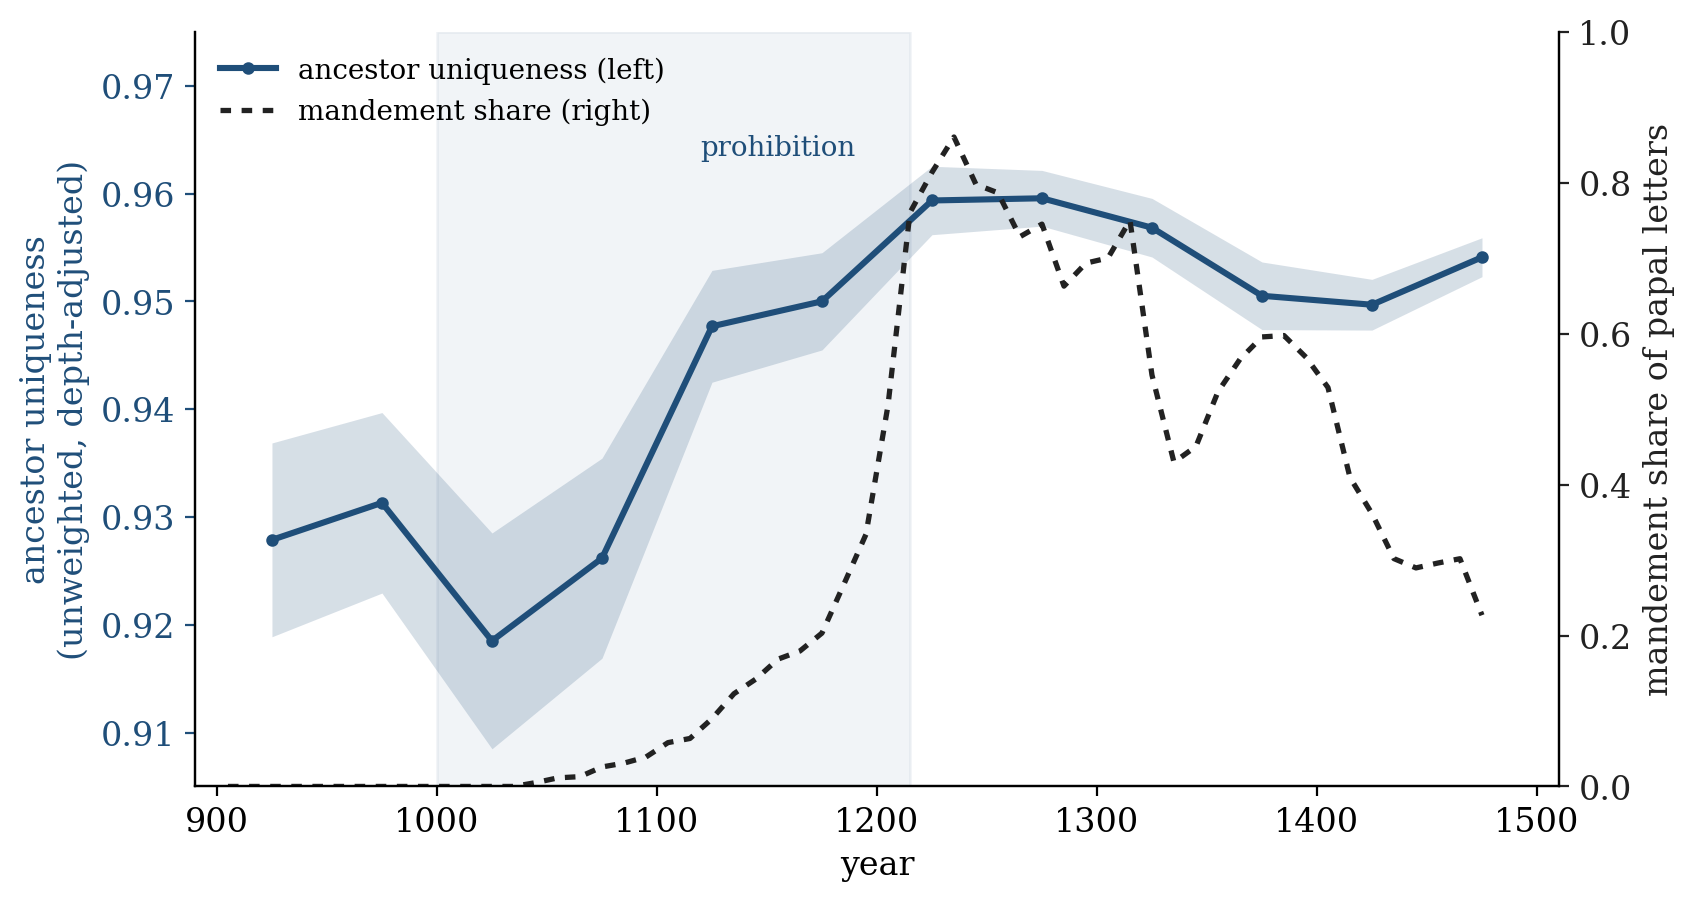
\includegraphics[width=0.9\linewidth]{figs/fig_comovement_anchorfree.png}
    \caption{Ancestor uniqueness (the depth-adjusted share of recorded ancestors who are distinct, 50-year birth cohorts) and the share of APOSCRIPTA letters that are mandements (50-year windows by letter date).}
    \label{fig:comove}
\end{figure}

Richer exploitation of the data confirms that interdynastic marriage drives papal involvement in dispute resolution. I develop a measure of kin-reach by subdividing a graph of \textit{The Peerage} genealogy into distinct kinship blocs on the basis of network topology. A noble's \textit{kin-reach} is the number of distinct blocs he reaches within a specified graph distance. For my main analysis, I define a kinship hop as one traversal of a parent-child or spouse edge, and define a noble's kin-reach as the number of blocs reached within four hops. I map the network of nobility alive 1100--1300 and instrument each male noble's kin-reach with the network he inherits maternally at his birth, with controls for plausibly confounding channels. Each additional bloc reached within four kinship hops raises a male noble's expected number of appearances in documents related to secular territorial conflicts by $3.3$ percent ($p = .005$); the effect is consistently stronger than the effect of reach on appearances in documents of any other subject, and it is uniquely robust relative to the effect of reach on appearances in other kinds of documents. These latter facts discriminate in favor of my theory (where exogamy drives demand for arbitration) and against a selection-driven relationship where exogamy is generally correlated with prominence in papal correspondence. The effect is concentrated among nobles who can be independently identified as conflict-prone and is robust to the omission of any bloc or noble as well as to randomization inference, though marginal under conservative cluster bootstrap specifications.

Moreover, my theory requires that the demand for law spread through the kin network through two channels. First, rival exogamy creates ambient risk. A noble who does not alter his own marriage strategies still may face a rival with highly variable support. Second, arbitration requires consent of both parties; therefore rival arbitration should drive own arbitration as arbitration opt-in cascades. I test this by measuring the \textit{breadth} of rival alliances by counting the mean number of distinct blocs within one hop of each other noble in a noble's four-hop range. That is, \textit{reach} measures how many different blocs a noble reaches, where \textit{breadth} measures how mixed up those blocs are with each other. A noble with high breadth faces rivals whose interests are diffuse and more difficult to coordinate, but who could potentially call on a wide range of families for support. I then regress a noble's appearances in secular territorial conflict documents on breadth and, separately, on the average number of appearances his rival has. The key result is that, while breadth predicts appearances in all eras, rival appearances strongly predict own appearances only before 1215 and not after (the post-1215 coefficient is in fact slightly negative). This shut-off is consistent with a cascade of opt-in to a network good: ambient risk persists, but the rival-generated incentive to adopt arbitration disappears when all possible rivals arbitrate, that is, when the network is saturated.

My argument contributes to a number of related literatures. Most obviously, \citet{schulz_2019, schulz_2022, henrich_2020} have documented the long-run cultural effects of the church’s “marriage and family program.” I isolate what I call the \textit{extreme marriage and family program} (EMFP) from 1003--1215, and document its political economy effects: mandated exogamy has profoundly disruptive legal effects where marriage is an important means of diplomacy. My argument complements the cultural account by grounding the church's legal authority; indeed, the church may only have been able to generally impose its policy, producing the cultural effects, because of its legal jurisdiction.

Second, my argument amounts to a theory of the West’s politico-legal distinctives with implications for long-run growth.\footnote{See \citet{koyama_rubin_2022} for a more comprehensive overview of the historical approach to development, and \citet{becker_rubin_woessmann_2024} for discussion of the general relationship between development and religion.} My argument is structurally similar to that of \citet{bazzi_koehlerderrick_marx_2020}, in that it attempts to ground religious institutions as political equilibria. In comparison, most other theories of Western institutional distinctiveness identify proximate causes of Western European development that take religious institutions as exogenous. For instance, church-constrained political authority \citep{rubin_2017} requires a church with jurisdictional authority. Relatedly, nuclear-family-based commerce \citep{greif_tabellini_2017} requires the European dissolution of archaic kin-based political structures; the same is true for the comparative arguments of \cite{kuran_2011} and \cite{blaydes_chaney_2013}. These accounts take either European kinship or ecclesiastical jurisdiction as primitive; my theory explains the primitives of these theories by taking the extreme consanguinity prohibition and Western European political fragmentation \citep{fernandezvillaverde_koyama_2023} as primitive. More distally, the market-for-ideas \citep{mokyr_2016} requires politically independent universities, which depend, like guilds \citep{delacroix_doepke_mokyr_2018}, on certain preexisting legal forms. \citet{ajr_2001, acemoglu_robinson_2012} emphasize the long-run force of inclusive institutions but take the historical emergence of European inclusivity as given; analogously \citet{north_thomas_1973} argue that property rights drive growth but take variation in property rights as largely given. Insofar as these institutions require more fundamental medieval legal institutions, my argument provides new grounding for long-run development claims.

Third, my argument reframes our understanding of medieval law and economics. Against \cite{ekelund_1996}, I argue that the medieval expansion of law was demand-driven from below, not rent-extraction -- in my model, the church acquires jurisdiction just insofar as it offers a valuable service. Where \cite{davray_2024} makes qualitatively similar criticisms of Ekelund et al., I provide empirical evidence. \citet{benson_1990} and \citet{milgrom_north_weingast_1990} discuss the evolution of the Law Merchant. \citet{berman_1983} traces the origins of medieval commercial law and argues that it owes much to the earlier canon law, not only in form, but also in that the appellate jurisdiction of canon law courts made possible medieval commercial contracts. Indeed, most  contracts in the 12th and 13th centuries included clauses that renounced recourse to any secular court in favor of ecclesiastical courts \citep[223]{berman_1983}. Similarly, \citet{goody_1983} famously argues that the church's kin-marriage prohibitions were designed to produce heirless houses that left their property to the church. Whether or not this claim is true, it relies on a legal framework in which the church has secure property, which is exactly the fact that I aim to explain. \citet{greif_rubin_2024} have a somewhat different conception of the church's distinct political role; they frame the church as a legitimator as opposed to arbiter. I see our respective accounts as complementary. Ecclesiastical legitimation works for precisely the same reason that arbitration works -- the legitimator/arbiter is credibly impartial -- and breaks down for precisely the same reason as well -- the legitimator/arbiter loses its credible impartiality.

Finally, my argument significantly extends the study of self-governing orders \citep{greif_1989, greif_1993, greif_milgrom_weingast_1994, boettke_2005a, boettke_2005b, greif_2006, boettke_candela_2019, boettke_candela_2020}. A large literature \citep{friedman_1979, ostrom_1990, ellickson_1991, bernstein_1992, leeson_2007a, leeson_2007b, leeson_2007c, stringham_2015, geloso_leeson_2020} identifies the viability of purely consensual mechanisms of governance in certain cases. I furnish this literature with a more general case study. By my argument, the foundation of the Western legal patrimony is consensual in nature: elites contract among themselves to economize on the costs of competing for rents by mutually agreeing to third-party legal procedures. Ecclesiastical jurisdiction was largely noncoercive and relied -- just as the Icelanders in \citet{friedman_1979} -- on the threat of outlawry (in this case, via excommunication). In other words, law is neither the mere imposition of the will of the strong, nor is it fundamentally contractarian. Law emerges, as \citet{hume_1739} and \citet{hayek_1973} have argued, spontaneously.

The rest of this paper proceeds as follows. Section 2 documents the history of the EMFP and ecclesiastical law, and summarizes my theory and its predictions (a fully formalized version of the theory and predictions appears in Appendix~\ref{app:theory}). Section 3 describes the construction of the major measurements of exogamy and demand for papal arbitration that Section 4 uses in tests of the theory. Section 5 concludes with additional suggestive hypotheses the theory raises.
% ===== END sections/Introduction =====



% ===== BEGIN sections/The medieval origins of Western law =====
\section{Medieval origins of Western law}
\label{sec:history}

\subsection{The puzzle of ecclesiastical jurisdiction}

\citet{southern_1970} observes that ``The [medieval] church was a compulsory society in precisely the same way as the modern state is a compulsory society" (17). But the church, unlike the modern state, governed organizations whose militarization and consequent capacity for projecting violent force exceeded (often vastly) the capacities of the church:
\begin{quote}
To rule men at a distance requires an army of willing and disciplined collaborators, capable of being reached by a word of command, of moving when commanded, and of coercion when necessary... But [popes] failed to gain the acquiescence which must be the basis of any state. There was a further ultimate impotence that prevented the medieval church-state from becoming a police-state. It had no police. It had no dependable army. \citep[19]{southern_1970}
\end{quote}
Thus the church was unlike a modern state in that it lacked any means of systematically initiating coercion. Its chief tool of discipline was excommunication. The church was an enormously powerful political force that incorporated the whole of medieval society, and yet did so, effectively, on the basis of the voluntary submission of its members, the most important and interesting of which seem like they could have acted with utter impunity given their comparatively great capacities for violence. This state of affairs, moreover, came to be only after an 11th-century reorganization of the church in relation to the secular elite.

Kings, not Popes, were the vicars of Christ until the 11th century \citep[32]{southern_1970}, and Christian piety dictated the submission of the church to the rulers which God had placed on earth for the direction of temporal affairs. \citet{southern_1970} quotes a representative political thinker from the turn of the millennium: ``Our kings and emperors, vicars of the Supreme Ruler in this pilgrimage, are alone responsible for the appointment of bishops, and this is right, for it would be incongruous if the pastors, who rule in the likeness of Christ, were set under the authority of any except those who are set above other men by the glory of benediction and coronation" (32). Centuries earlier, Charlemagne is acknowledged to be ``in power more excellent than the pope or emperor in Constantinople, in wisdom more distinguished, in the dignity of your rule more sublime" (32). How, in such a world, could Emperor Henry IV find himself kneeling in the snow for three days before the Pope's gates in Canossa in a desperate bid to lift his excommunication? How could it be reasonable for Henry II of England to walk barefoot to Canterbury in penance for Becket's murder? How did there come to be ``in Rome a single spiritual and temporal authority exercising powers which in the end exceeded those that had ever lain within the grasp of a Roman Emperor" \citep[25]{southern_1970}? To chalk up the power of the Roman church to fear of punishments in the afterlife is similarly misguided: ``fear of spiritual sanctions cannot explain the phenomenon [of ecclesiastical governance]. Such fear... was a result rather than cause of the growth of papal government" \citep[25]{davray_2023}. The puzzles of ecclesiastical authority and the power of excommunication are one and the same.

Growth in ecclesiastical authority in Western Europe was demand-driven, on two levels. First, lower level clerical elites demanded dispute resolution from an impartial third party: Rome \citep{davray_2023}. Second, secular elites increasingly demanded clerical dispute resolution \citep{davray_2010}. These two facts led to a state of affairs where the clergy in general functioned as representatives of Rome for the resolution of disputes across Western Europe, with Rome functioning as an appellate court. \citet{berman_1983} writes

\begin{quote}
    The relatively unsystematized character of legal regulation [pre-1000]... was closely connected with the prevailing political, economic, and social conditions. These included the predominately local character of tribal, village, and feudal communities; their relatively high degree of economic self-sufficiency; ... the relative weakness of the political control exercised by the central imperial and royal authorities; ... \textit{and the relative strength of informal community bonds of kinship and soil and of military comradeship}... Thus, the creation of modern legal systems in the late eleventh, twelfth, and early thirteenth centuries was not only an implementation of policies and theories of central elites, but also a response to ``changes on the ground." (87, emphasis added)
\end{quote}

 \citet{davray_2023} similarly argues:

\begin{quote}
    The rise of academic Roman law... coincides closely with a massive expansion of papal government, driven by demand from below, a widespread tendency to fight litigation to the highest court, and a desire for authoritative case law. While there is no obvious direct causal relationship between these two developments, there is an indirect one and a kind of affinity. The papacy found certain key Roman-law concepts to be a powerful instrument for meeting the demand for high-level justice. (134)
\end{quote}

Elsewhere, \citet[38]{davray_2023} shows that the vast majority of papal documents between 400 and 1600 -- noting an explosion in volume in the late eleventh century -- were responses. The papacy was not primarily in the business of legislating, but of adjudicating.

What is missing from existing stories about the growth of ecclesiastical law is an explanation as to where the demand came from. To some extent, as \citet{davray_2023} notes, there was always demand for papal dispute resolution. But before 1000, this demand was primarily concentrated within the church, and was extremely small compared to the High Middle Ages. My theory explains the demand shift.

\subsection{The legal transformation}

The key features of the legal transformation are worth describing in some detail. 11th-century scholastic canonists developed the methodological innovations that made canon law a usable instrument of dispute resolution across Latin Christendom. Chief among these were systematic concordance of canons, precisely delimited jurisdictions, and hierarchical appellate review. Canonists then asserted the jurisdiction of the church to secular disputes. Feudal lords had long held jurisdiction over their tenants' disputes, but the church asserted jurisdiction in any case where the disputants were wards of the church, such as widows, orphans, and the poor. Canonical legal concepts were in turn absorbed into feudal, urban, and commercial law; the church's courts became the appellate venue across a vast class of cases. \citet{berman_1983} notes that ``prior to the mid-eleventh century, lord-vassal relations and land tenure... were not subjected to systematic legal regulation" (297); by the 12th century, feudal law had transformed such that vassals gained codified rights assertable against their lords, and ``feudal law gave the West its first secular experience of the mutuality of legal obligation between persons of superior and inferior rank" (309). The aristocracy became, in response, extremely litigious \citep[309]{berman_1983}; see also \citet[40]{heer_1962}.

Several mechanisms reduced the partiality of clerical elites, enabling them to credibly adjudicate disputes across Western Europe. First, the growing hostility to clerical marriage and fatherhood separated clergy to some extent from secular politics: their own family ties could not be reinforced through the betrothal of their children when they had none, nor could they develop marriage ties with other potential allies. In ``the first great age of propaganda" \citep[xiv--xv]{bennett_1936}, the church issued pamphlets and organized preaching campaigns warning against receiving any sacraments from priests who lived with women. Not incidentally, this project was spearheaded by the monk Hildebrand, who became Pope Gregory VII, and under his papacy ordered all faithful Christians to boycott the services of married clergymen, resulting in riots and stonings (both on behalf of and against married priests). The problem as Gregory VII saw it was that ``marriage brought the priesthood within the clan and feudal structure" \citep[90]{berman_1983} -- that is, it was a threat to the independence of the church.

Second, a legal infrastructure developed in which intramural ecclesiastical crises were resolved by higher level authorities (ultimately, Rome) reducing the autonomy of local agents of the church, who nonetheless retained jurisdictional authority that Rome could not usurp. While Rome had served historically as a court of appeals of sorts in disputes within the ecclesiastical hierarchy, its authority to do so was by no means a matter of course. When monasteries or bishops wrote to the Bishop of Rome to request some kind of judgment, they did so without acknowledging Rome's \textit{general} right to judge; Rome had authority in particular cases by virtue of the mutual submission of disputants to Rome's decision, not by any sort of divine right \citep{davray_2023}. This was especially the case by 1000, when the Eastern churches had long since ceased to acknowledge any distinct authority in Rome, and the dioceses in the Western church saw royal and imperial authority as outranking that of the Pope. Gregory claimed, however, that papal court was ``the court of all Christendom" \citep[7]{bernheim_1896}. To make good this latter claim, Gregory also oversaw the beginnings of a dramatic expansion and formalization of the church's legal procedures: under Gregory and his successors, ``the church interpreted its laws and applied them through a judicial hierarchy culminating in the papal curia in Rome" \citep[113]{berman_1983}. The hierarchy was staffed by papal representatives, and their representatives, in a manner not unlike the organization of a modern regulatory bureaucracy under an executive.

Third, the development of the canon law rigorously proceduralized litigation in such a way as to make legal reasoning amenable to public evaluation; and judges could be sued for the miscarriage of justice. Fourth, monastic pressure on episcopal election plausibly constrained episcopal rent-seeking \citep{shera_2025}. Fifth, a papal crackdown on simony (sale of church offices) and a prohibition on land alienation meant that ecclesiastical elites were significantly limited in their capacity to directly extract rents from their authority; their incomes depended upon their continuing to hold office. I thus characterize the legal apparatus of the church as consisting of a rules-based system for adjudicating disputes managed centrally by Rome, whose own authority derived principally from its reputation for providing law.

The church thus offered a high-quality dispute-resolution product, especially relative to the secular alternatives. Its product quality was, however, in large part contingent upon the number of its purchasers; a system of law is a network good in that it is only valuable insofar as counterparties can be expected to abide by court rulings. But if a network good is sufficiently demanded, then the threat of exclusion from the network is powerful. The church called such a penalty \textit{excommunication}. \citet{vodola_1986} and \citet{helmholz_1982} observe that oaths taken by an excommunicate were invalid, and therefore, that the excommunicate could not serve as witness, plaintiff, or defendant in a court of canon law. Excommunication was outlawry.

By the end of the eleventh century, excommunication had been fully proceduralized 
\citep{helmholz_1982}. Sentences of excommunication could only be passed after due process in an ecclesiastical court; sentences were subject to appeal at higher courts (the highest appellate court being, of course, Rome); excommunications could only be issued after summons to court by citation in writing; sentences also had to be in writing, with reasons for excommunication, and the excommunicate was entitled to a written copy of his sentence; the excommunicate had the right to seek remedy if procedural rules were not observed; the remedy might or might not undo his excommunication, but he might be awarded damages regardless, if, for instance, the court was found to lack jurisdiction, or had not served him a written citation \citep[204--205]{helmholz_1982}.\footnote{This worked through a special kind of absolution called absolution \textit{ad cautelam} (``for caution"). Though the excommunicate was in principle altogether denied access to law on grounds of his excommunication, if his excommunication was unjust, then he was not really excommunicated in the first place. So he was absolved of his excommunication just insofar as he claimed his excommunication was unjust, until the appellate court heard and decided his case \citep[206]{helmholz_1982}. In other words, the system of canon law provided an exception to its exclusion penalty to allow anyone to challenge his excommunication, and possibly recoup damages from the judge who had unjustly excommunicated him.}

The canonists moreover generally came to agree that excommunication should be reserved for the contumacious -- that is, those in contempt of court. Sentences of excommunication should be passed chiefly upon those who either failed to respond to a court summons or who failed to comply with a judgment. The exceptions to this guidance were for particularly egregious sins for which one incurred automatic excommunication, of which incest was one. Sentences should be  promptly lifted, moreover, upon the excommunicate's compliance. Evidence from England suggests that excommunications were used principally for just that and lifted without further penalty or ado upon the compliance of the excommunicate \citep[214]{helmholz_1982}.

Throughout the 11th century -- including especially but by no means limited to the period of the Gregorian Reforms (1073--85) -- the church transformed itself into a vehicle of law. Its chief spiritual sanction, excommunication, became a legal sanction.


\subsection{The Extreme Marriage and Family Program}
Two strains of teaching influenced the church's perspectives on incest. The church had long prohibited incest between third cousins and closer kin on grounds of ritual impurity. A fifth century argument from Augustine of Hippo (\textit{City of God} XV.16) decried endogamy on political grounds: marriage within a family constituted a failure to extend Christian charity to one's neighbors. The church accelerated its marriage and family program in the 11th century when Holy Roman Emperor Henry II sought to break up the marriage alliances of his unruly nobles \citep{ubl_2008}. In this effort, he was aided by the canonist Burchard of Worms, whose \textit{Decretum}
\begin{quote}
conflated two traditions that hitherto had been separate. Those early medieval councils that so strongly expressed fear of incest as a source of ritual impurity were referring to incest prohibitions significantly more limited than those Burchard propagated, while his authorities in favour of the very wide definition of kinship were not equally concerned with purity and pollution, if at all. \citep[154]{rolker_2012}.
\end{quote}
Canonists repeatedly combined ritual horror with arguments for the political value of exogamy to pursue an expansive definition of \textit{kin} that included sixth cousins, affines, and fictive kin like godparents. Specifically, they argued strongly for a ``seven-degree" prohibition: couples could not share a common ancestor within seven preceding generations (i.e., could not be sixth cousins or closer).\footnote{The exact argument of the canonists exploited a discrepancy in consanguinity degree-counting techniques. The earlier prohibition covered couples related within four degrees of consanguinity -- couples who shared an ancestor within four generations (third cousins). But one could alternatively count up from one spouse to the common ancestor, and then back down to the other spouse. In this case, a third-cousin marriage is at the eighth degree of consanguinity: starting from one spouse, count three or four generations up to the shared great-great-grandparent, and four generations back down to the other spouse, for a total of eight. In fact, where this counting method was employed, law restricted marriages to those who were not related within seven degrees, so a seven-degree prohibition by what is now called ``Roman" counting (up-then-down) is slightly less restrictive than a four-degree prohibition by what became the ``canonical" method (up only). What the canonists seem to have done, then, is argued that the then-widespread seven-degree prohibition was correct, but the proper method of counting was to count generations only up to the nearest common ancestor (an older method of counting), producing a geometrically more restrictive seven-degree prohibition.} The first clear case of the prohibition occurred at a council (called by Henry II) in Diedenhofen in 1003.

Historians have tended to emphasize the political motivation. For instance, \citet{esmark_2020} argue that ``the introduction of canonical kinship was inspired by Christian peace ideology and aimed to limit the allegedly endless feuds and social conflicts among the elite, not only between rival aristocratic families but also internally between affines and blood relatives" (23). Later canonists' own reflections are similar. A 20th-century canonist discusses the role of medieval consanguinity law as follows:
\begin{quote}
    The Church was prompted by various reasons first to recognize the prohibitive legislation of the Roman State and then to extend the impediment of consanguinity beyond the limits of the civil legislation. The welfare of the social order, according to St. Augustine (City of God XV.16) and St. Thomas (Suppl. Q. liii, a. 3), demanded the widest possible extension of friendship and love among all humankind, to which desirable aim the intermarriage of close blood-relations was opposed; this was especially true in the first half of the Middle Ages, when the best interests of society required the unification of the numerous tribes and peoples which had settled on the soil of the Roman Empire. By overthrowing the barriers between inimical families and races, ruinous internecine warfare was diminished and greater peace and harmony secured among the newly-converted Christians. \citep{burtsell_1908}
\end{quote}

In general, the sin of incest incurred excommunication. Synods across Europe began to condemn as incest all marriages where the spouses shared seven degrees of consanguinity on pain of excommunication, in the wake of Diedenhofen and Burchard's \textit{Decretum}. Famously, Pope Nicholas II published an encyclical in 1059 officially ruling that anyone who married within the seventh degree of kinship would be forced by his bishop to separate or face immediate excommunication.

\citet{davray_2005, davray_2014, davray_2015} extensively documents the use of the prohibition to facilitate strategic divorces. Though marriages were in principle indissoluble, couples could -- and regularly did -- secure annulments on grounds of consanguinity. D'Avray further shows that the widespread abuse of the system prompted the church to reduce its prohibition to the earlier third-cousin (four degrees of consanguinity) rule at the Fourth Lateran Council in 1215.

\subsection{Kinship and politics}
For medieval nobles, relations of marriage functioned as a sort of bilateral hostage exchange. That is, the families of married couples tended to have some sort of leverage over each other. The wife was sent to her husband's court — a literal hostage — where she then exerted influence over her husband and his courtiers. The parties to the marriage gained the power to assert claims on each other; and for politically engaged families, one important kind of assertable claim was for political support.

An out-of-network marriage (exogamy) could secure a new ally, but this ally would have competing commitments, and the arranger of the marriage forgoes the opportunity to prevent another one of his existing allies from acquiring a competing interest. An endogamous noble with many in-network marriages could expect to be supported by a smaller maximum and larger minimum of his putative friends. He did not have as many people in his network, but each one had fewer competing commitments; their support was thus more reliable. In-network marriage thus functioned analogously to insurance — nobles might forgo larger alliances in favor of more committed ones, to minimize randomness in political support. This observation invites a further one about the macrocosmic alliance structure: if the average level of exogamy increases above the alliance-optimizing level, then political conflict should exhibit more randomness. It becomes ambiguous who is whose ally when the entire network is intermarried.

Existing work by historians and anthropologists complements the foregoing description. \citet{hermanson_orning_2020} argue:

\begin{quote}
The establishment, maintenance, and dissolution of networks constituted the core of high medieval politics... Networks functioned as \textit{socio-political assurances}, since their members could rely on support and protection in the event of a conflict breaking out. Networks contributed to \textit{predictability}, making it possible to estimate one's own and one's opponent's resources, and to anticipate the actions of an enemy. (59, emphasis added)
\end{quote}

Network construction facilitated predictability by the provision of assurances, which is to say, network construction reduced risk by creating credible commitments. \citet{halden_2020} characterizes kinship groups as the central unit of medieval political order. Moreover, the importance of kinship ties extends to the highest level of politics: the European aristocracy was a ``network of family networks" from which ``kings were not isolated" (120). \citet{hornaday_1996} finds that the battle lines in Germanic and Irish feuds tended to divide fairly neatly between kinship groups, with the exception of royal feuds, in which the royal family was at war with itself; even then, aristocratic families would still tend to choose sides as cohesive units themselves. \citet{lejan_1998} further argues that ``political relationships" had been reconstructed by ``the weakening of the state since Antiquity" on ``a logic of personalized bonds that entailed reciprocity: an exchange of services between groups and individuals" (63), including, importantly, family networks. None of this is to suggest that kin-groups never dissolved into internal war; on the contrary, it is precisely because of this threat that kinship ties demanded redundancy.

My argument is that the EMFP established a feedback mechanism. If kin-groups blurred for any reason, the allies of any one noble became implicated in his rivals' alliances; the insurance function of in-network marriage decayed. To economize on these dispute costs, nobles substituted out of the direct negotiation of conflict and into arbitration; the highest-quality arbiter was the Roman church. But to access ecclesiastical courts required communicant status; to be communicant required compliance with canon-law marriage rules. Thus, as demand for law increased, nobles further increased their exogamy, further increasing demand for law. The process continued until the Fourth Lateran Council in 1215, by which point the church had established canon-law jurisdiction firmly enough that it could afford to relax the marriage rule to its pre-EMFP level. By then, however, the aristocracy had access to law, and there was no reason to re-form tight-knit kin-groups. The pattern of exogamy remained broadly locked in, and the church maintained its widespread jurisdiction.

I formally model this theory in Appendix~\ref{app:theory}. The verbal model delivers the following qualitative predictions (I derive these formally in the appendix).
\begin{enumerate}
    \item \textit{Exogamy drives demand for law.} Inheriting a more exogamous network should cause a noble to seek more arbitration, relative to nobles who inherit less exogamous networks.
    \item \textit{The demand for law spreads through the network.} A noble born into a broader, more court-engaged kin network should seek arbitration more, through two channels. First, his peers' resort to arbitration makes the court more valuable to him. Second, their exogamy makes force riskier for him. While the EMFP builds the network, exposure to peers' prior arbitration should predict a noble's own arbitration. Once arbitration is general, after the EMFP, that prediction should disappear, while the risk channel, which depends on the population's exogamy rather than on who has litigated, should persist.
\end{enumerate}
I test these predictions below.
% ===== END sections/The medieval origins of Western law =====



% ===== BEGIN sections/measure_section_7_1_26 =====
\section{Data and measurement}
\label{sec:measurement}

To test the theory, I recover two quantities from the historical record: the exogamy of each noble's house and the church's involvement in settling noble disputes. I build the first from a genealogy of the European aristocracy and the second from the surviving corpus of medieval papal letters. This section describes both constructions.

\subsection{Two sources}

\emph{The Peerage} \citep{lundy_2024} is a continuously updated genealogy of the European nobility, which I scraped in August 2024 to a graph of $727{,}753$ individuals. Each person is a vertex; an edge joins a parent to a child and a spouse to a spouse. The graph provides a broad window on the kinship structure of the Western aristocracy.

APOSCRIPTA is a scholarly corpus of $25{,}190$ medieval papal letters; $24{,}130$ fall in the era from which I extract matches (1020--1380), and $21{,}584$ in the analysis window of 1100--1300. Each letter carries an editorial summary, a date, and, where it survives, a transcription of the Latin. To measure an individual noble's engagement with ecclesiastical organs of dispute resolution, I match nobles in \emph{The Peerage} to the persons named in these letters, as described below.

\subsection{The motivating stylized facts}
\label{sub:facts}
Preliminary analysis of \textit{The Peerage} data documents that an enormous and permanent transformation happened in European aristocratic marriages between 1000 and 1215. Three distinct measures corroborate the same basic story: exogamy exploded around 1000, reached a saturation point around 1215, and then, very importantly, had not significantly attenuated by 1500. This latter fact is one key motivation for my theory; the fact demands an account of marriage practices that accommodates increasing exogamy in response to church policy, but not decreasing exogamy in response to the policy's relaxation.

The first measure is purely genealogical. The prohibition extended to seven generations; each person has a total of 254 possible ancestors within seven generations. For a fully outbred family tree, each of those 254 people is unique. With some level of inbreeding, the number of unique nobles will be less than 254. Unfortunately, data is not rich enough to identify all 254 ancestors within seven generations for most nobles. Therefore, I count $P$, the number of actually recorded ancestor slots, and $N$, the number of unique ancestors across recorded slots, in order to measure $\tfrac{N}{P}$, the fraction of recorded ancestors who are unique. I restrict my analysis to nobles who have at least six filled ancestor slots -- smaller lineages mechanically deliver $\tfrac{N}{P} \approx 1$. Because lineages are not sufficiently complete in the 800s, the plotted series begins with the cohort centered on 925. I pool nobles by half-century (by birth year), and plot the resulting measure of ancestor diversity.

I then modify this measure in three ways. First, and most importantly, I consider a depth-controlled version. Nobles vary in recorded depth. Mechanically, a noble with a relatively shallow lineage has fewer opportunities to record a unique ancestor occupying multiple distinct ancestry slots. By weighting nobles equally, the results are thus biased upward whenever lineages are sparse; new lineages have small depth and therefore a mechanically high $\tfrac{N}{P}$. The bias declines over time as average lineage depth extends; over time, then the bias results in understated growth in exogamy pre-1215 and mechanical decline in exogamy after. To correct this, I regress each noble's $N/P$ on each noble's recorded ancestry completeness $P$ for the pooled sample of all nobles born between 800 and 1500 and adjust actual values by those predicted.\footnote{Specifically, the regression form is a cubic polynomial in $\log(P)$.} Second, I consider a weighted version, where ancestors receive a weight of $2^{-d}$, where $d$ is the ancestor's generational depth from the focal noble. Parents receive $d = 1$, grandparents $d = 2$, through great-great-great-great-great-grandparents at $d = 7$.\footnote{The weighted measure weights each distinct ancestor once at its shallowest depth in the numerator while the denominator weights every slot.} This weighting captures the genetic contribution of each ancestor; and while there is no reason to think that genetics are particularly important for strategic marriage alliance-building, it is a principled, conservative weighting scheme that captures the alliance-building intuition that more generationally recent endogamy might be more important. Third, I consider a combined weighted and depth-adjusted measure.

Figure~\ref{fig:ancestors} plots all four measures of ancestor uniqueness. All four are in broad agreement that ancestor diversity increased near-monotonically during the EMFP. The depth-adjusted measures remain persistently elevated after, but stop increasing. Because the number of nobles per cohort increases monotonically, it is not likely that this result is a mechanical artifact of simply better recording.

\begin{figure}
    \centering
    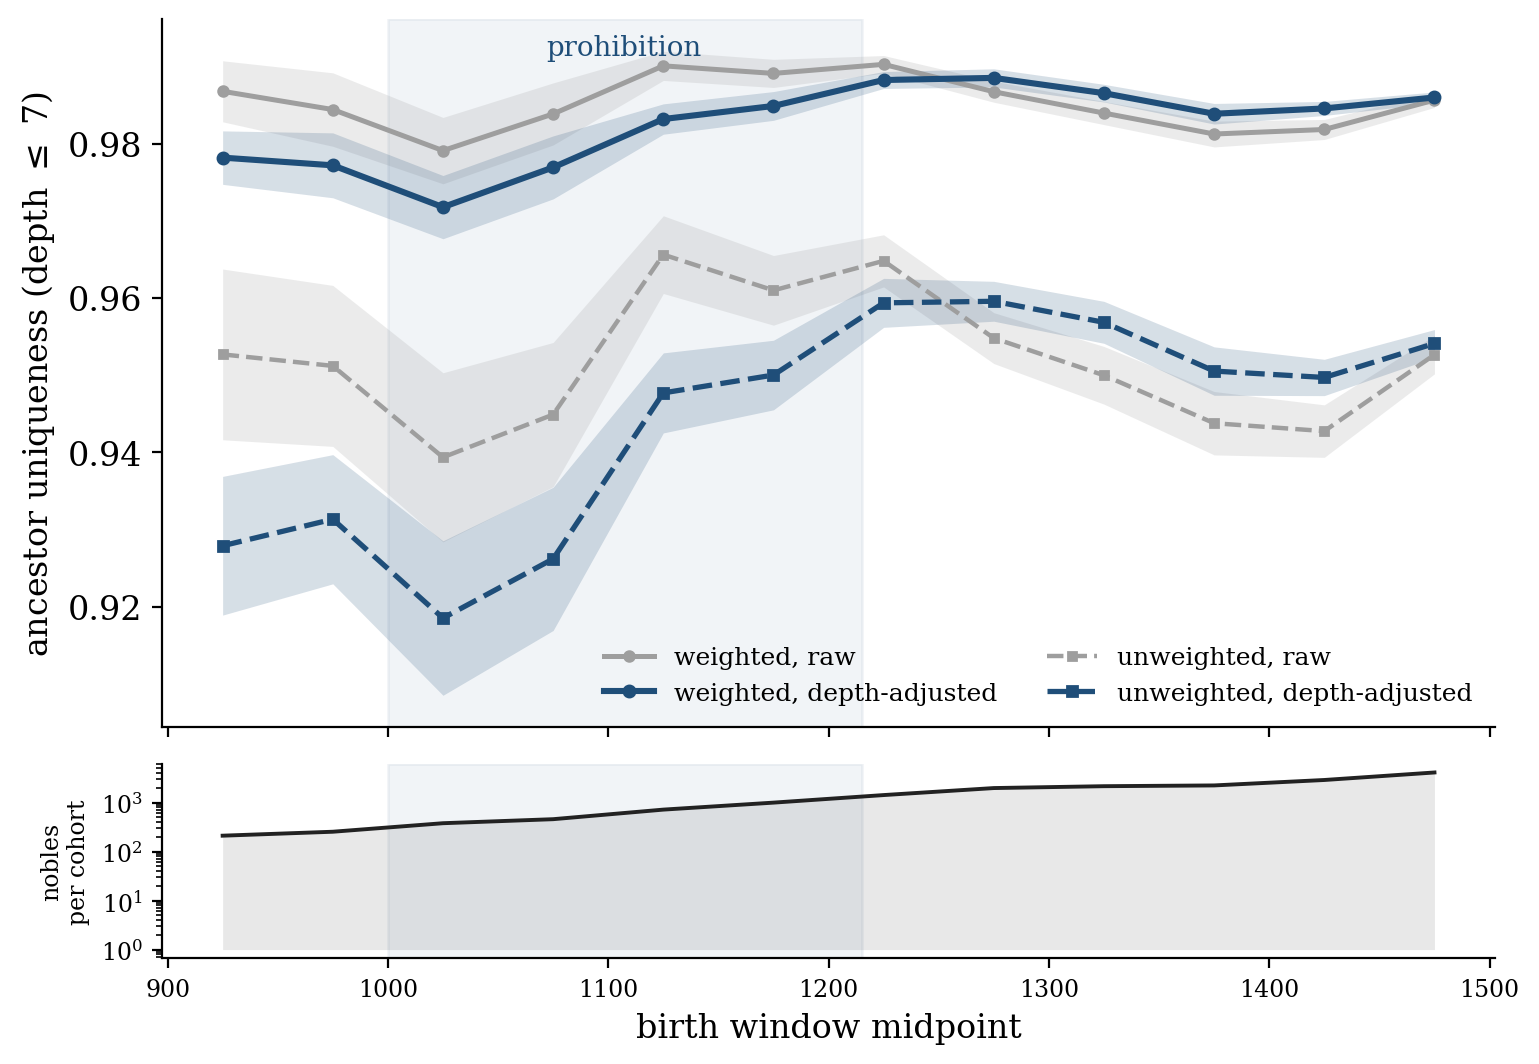
\includegraphics[width=0.9\textwidth]{figs/fig_ancestor_uniqueness_n.png}
    \caption{Four measures of ancestor diversity over time. Nobles grouped by 50-year birth cohorts, centered on window midpoints. The lower subpanel displays the number of observations per cohort on a log scale. Bands denote pointwise $95\%$ normal-approximation intervals for the cohort mean. $17,810$ total nobles with $\geq 6$ recorded ancestor slots plotted in this series (the adjustment is derived from a pool sample of $18,091$, including the earliest two omitted cohorts).}
    \label{fig:ancestors}
\end{figure}

Second, I consider a measure of exogamy based on pure network topology. I first divide the graph of the network into non-overlapping temporal subgraphs by 50-year birth cohorts (the graph of nobles born 800--849, then 850--899, through 1451--1500). Then, for each subgraph, I detect topological communities using the Leiden algorithm for community detection \citep{traag_2019}. Below, in Section~\ref{sub:reach}, I describe in some detail network modularity and procedures for community detection that optimize network modularity. For now, let it be sufficient that this method detects redundancy of connections among subsets of vertices in a graph; and that therefore, by the construction of the graph, it is particularly useful for identifying extended families. When sorting into communities, I omit connected components (that is, clusters of nodes entirely isolated from the rest of the graph) whose vertices are less than $1$ percent of the total number of vertices in the graph. I then count the number of community spanning edges: the number of edges in each subgraph that connect vertices who have been assigned to two distinct communities. Because the size of the graph changes -- increasing monotonically and exponentially over time -- my topological measure of exogamy is the ratio of the number of community spanning edges to the number of communities. Since Leiden communities are extended families, this measure is nicely interpretable as the number of cross-family kinship ties the average family has.

Leiden sorting can be biased in the sense that, as the number of vertices in a graph grows, Leiden sorting will mechanically find more communities. If detection refines the graph faster than the true number of families grows, later partitions will be more finely subdivided than the real family units. Thus, edges that are actually within an extended family might be counted as spanning communities, overstating the true number of spanning edges. To counteract this bias, I report a differently sorted series of graphs alongside it. I force Leiden to change resolution as the number of vertices changes, holding the number of communities $k$ roughly constant at about $25$. The bias here is of course in the other direction: holding constant the number of communities could mechanically reduce the number of community spanning edges. I report both results side by side in Figure~\ref{fig:leiden}. Since the two measures introduce opposite biases and yet are in substantial agreement, it is unlikely that a mechanical effect arising from arbitrary decisions in the coarseness of the partition drives the pattern. The remaining possible bias is that network growth is mechanically driven by improved documentation; this seems unlikely, as above, because the number of vertices grows monotonically over time, but growth in the number of spanning edges per community clearly plateaus around the 1200 cohort.

\begin{figure}[t]
\centering
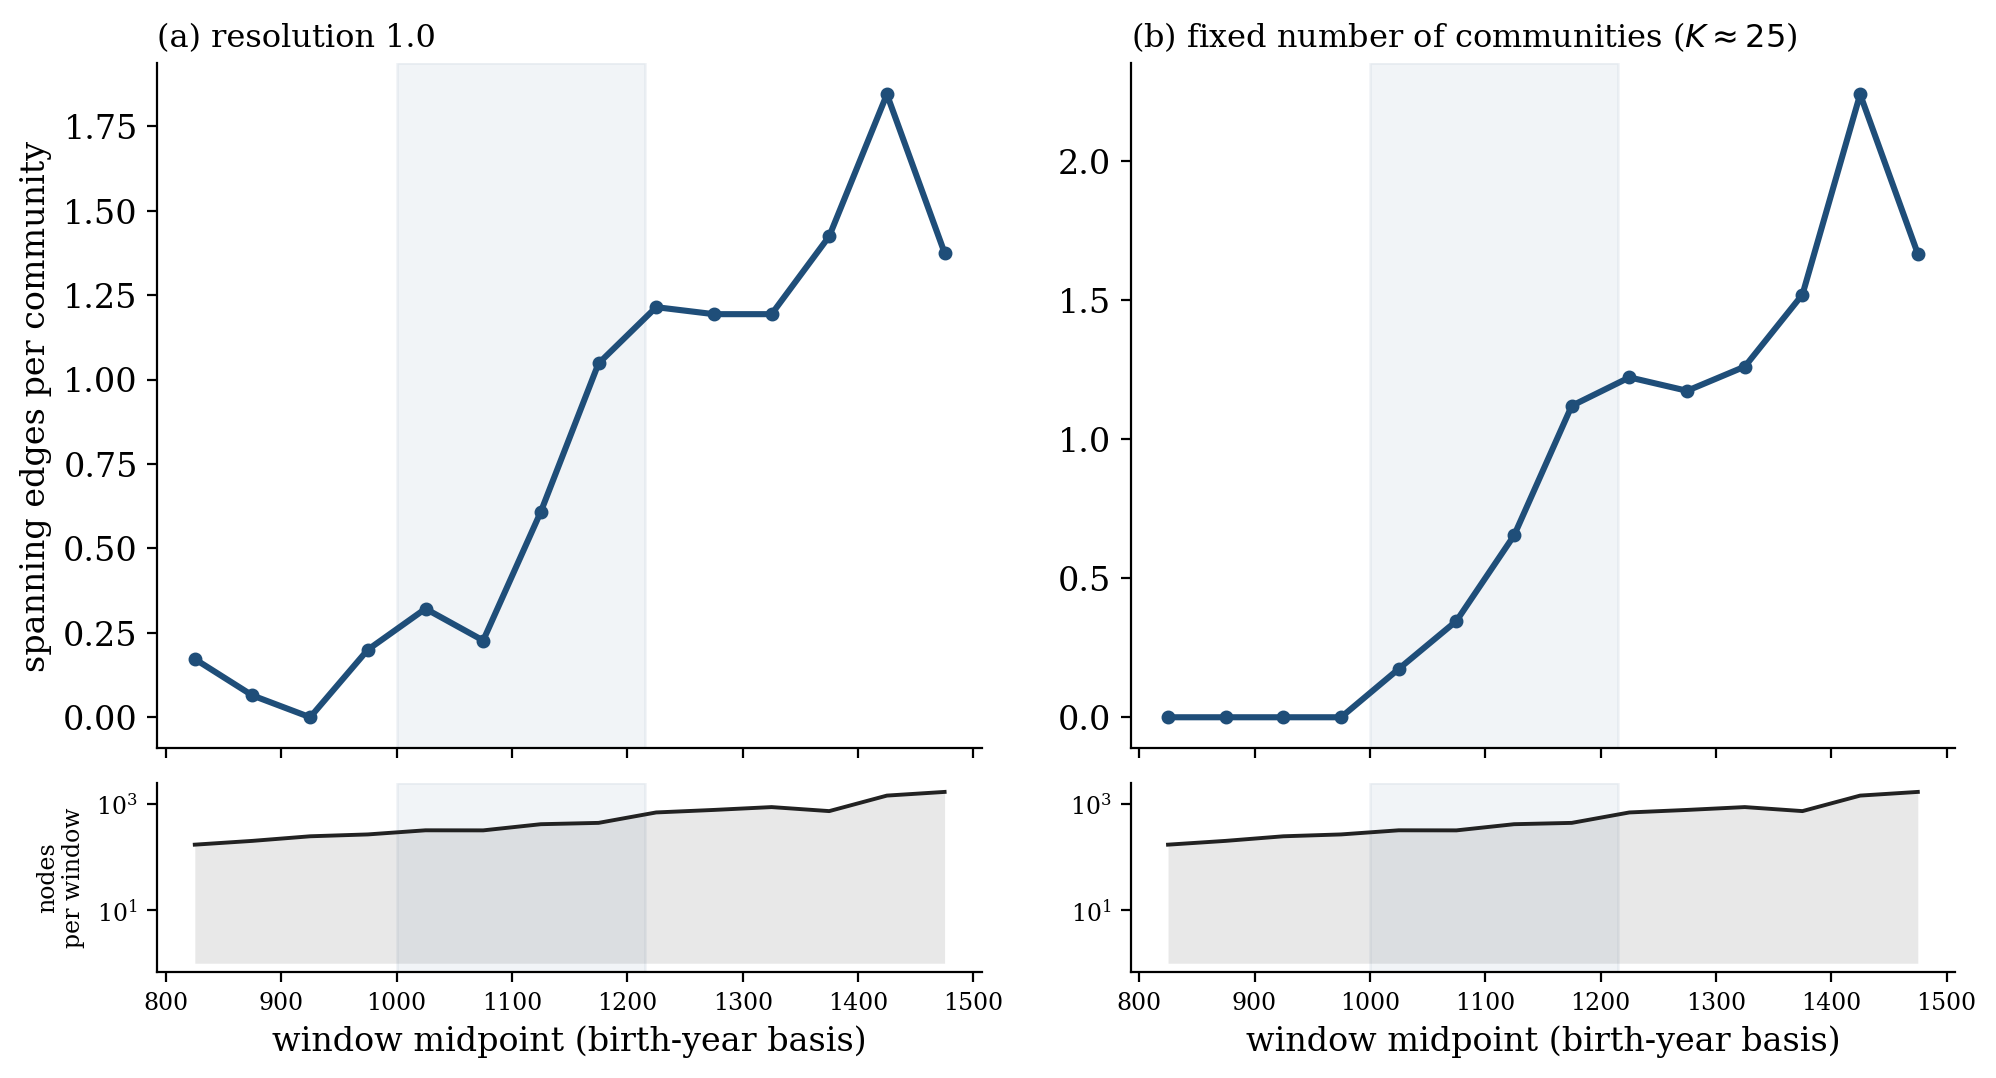
\includegraphics[width=\textwidth]{figs/fig_spanning_paper_n.png}
\caption{The exogamy trend in pure topology. Ties spanning distinct Leiden communities of the kinship graph, per community, in fifty-year windows by birth cohort, centered on window midpoint. Connected components smaller than $1\%$ of window nodes are filtered out. The lower subpanel displays the number of observations per window on a log scale. $8696$ unique nobles who have connections to components larger than $1\%$ of total vertices for their windows, summing across windows.}
\label{fig:leiden}
\end{figure}

Finally, I consider a measure that combines topology and genealogy with historically informed judgments about important ancestors. Observing the list of nobles who lived between 800 and 950, I curate a list of historically important dynastic founders. This produces $21$ distinct dynasties. I then create a graph that lacks spousal edges; the graph documents pedigree through parent-child edges. I assign all nobles within six kinship hops of any anchor, where one hop is one edge traversal on the pedigree graph (so, mother-to-son is one hop, mother-to-grandson is two), to the dynasty of the nearest anchor, with ties broken by the number of anchors the dynasty has (larger anchoring pools win).\footnote{Ties within this ordering are broken arbitrarily by a deterministic process described in the replication package.} Then, all nobles unreached by the six-hop breadth-first search inherit the dynasty of their parent who is closest in graph distance to the anchor. This procedure assigns all and only those nobles whose ancestry is genealogically traceable pre-950 to dynasties. I date each marriage by a proxy marriage year (the midpoint of the two spouses' death years) and compute the interdynastic marriage rate in rolling fifty-year windows stepped by decade; a marriage is interdynastic just if the spouses are assigned to different dynasties. The share is computed only for marriages where both spouses have an assigned dynasty and plotted over time in Figure~\ref{fig:interdyn}.\footnote{This fact implies that the share is biased downward as new families enter the genealogy. These families aren't anchored, so nobles who marry into them aren't recorded in the reported share -- but most of these marriages should likely be classified as exogamous. This fact probably explains the secular decline in interdynastic marriage post-1250 as well as makes the upward drift during the EMFP more striking.}

There is a sense in which this measure is obviously worse than the other two, because, first of all, tie-break rules are semi-arbitrary and could conceivably influence outcomes, and more worryingly, there are substantial researcher degrees of freedom involved in the selection of dynastic anchors. On the other hand, the method is superior in that it allows me to track marriages directly and it allows the assignment of dynasties to be historically informed. While it would be unwise to rely on this measure of exogamy alone, it is striking that it substantially corroborates the other two measures. Moreover, it is difficult to imagine that either researcher bias in anchor selection or bias in dynastic assignment tiebreak rules would mechanically produce the observed change around the 1200 cohort.

\begin{figure}[t]
    \centering
    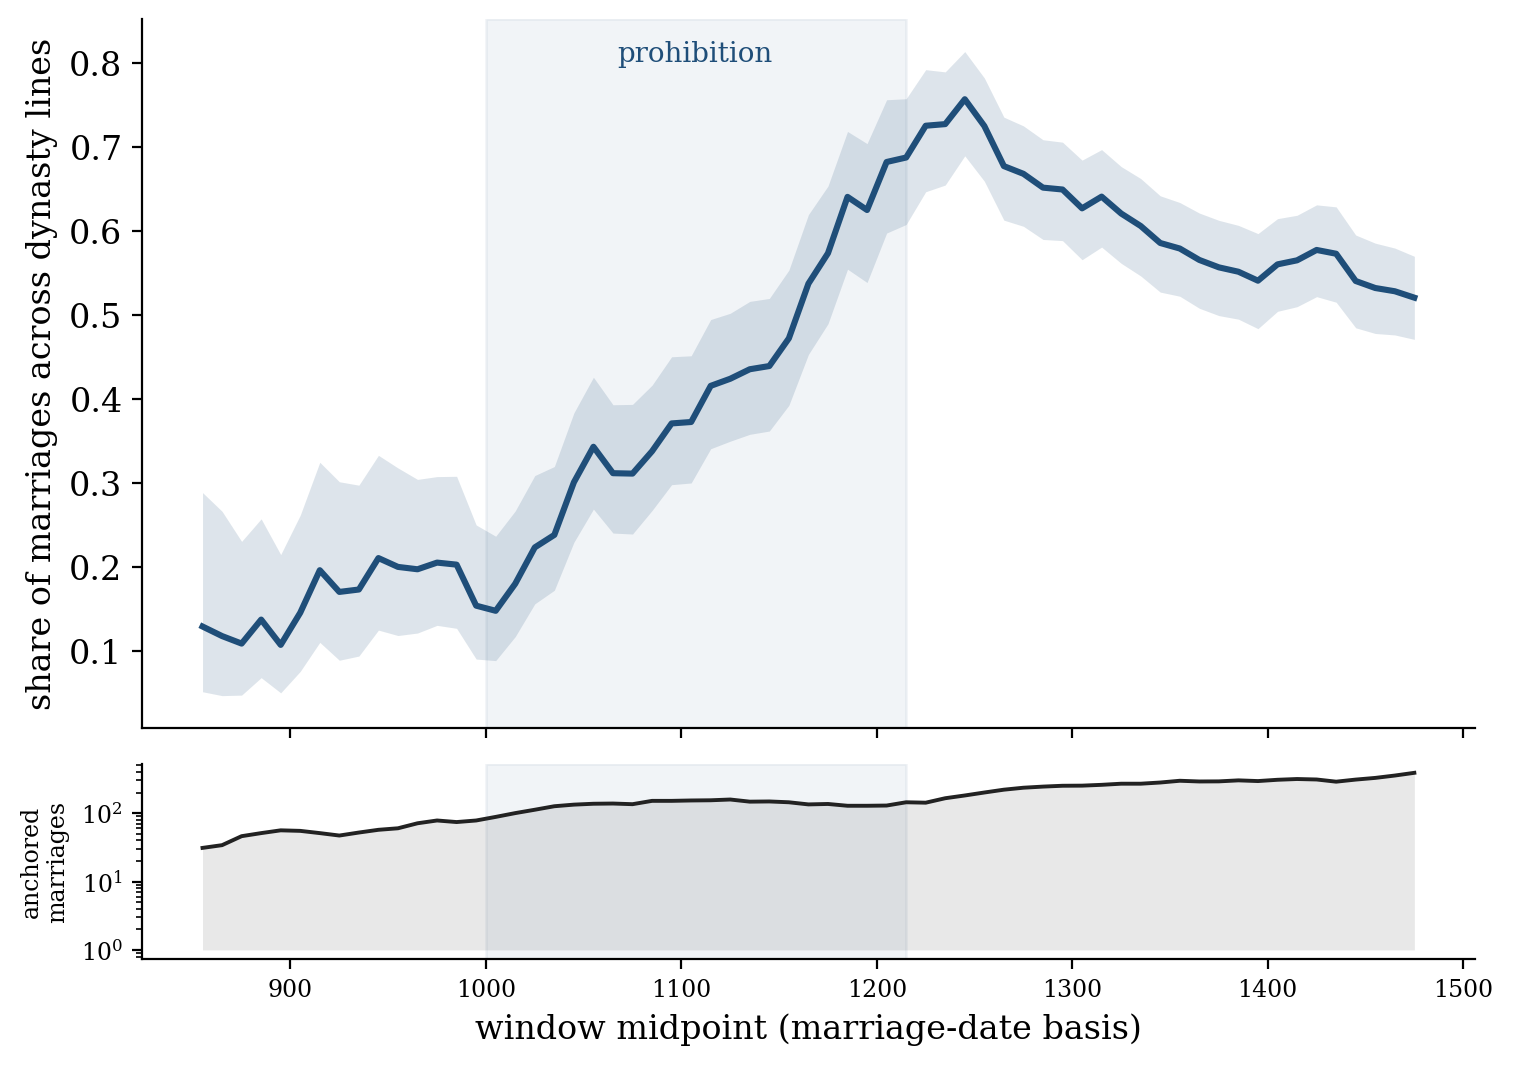
\includegraphics[width=.9\textwidth]{figs/fig_interdyn_n.png}
    \caption{The share of marriages that are interdynastic, in rolling fifty-year windows by proxy marriage year. The lower subpanel displays the number of observations per cohort on a log scale. The band represents a $95\%$ Wilson interval. $2380$ both-anchored marriages of $4,222$ unique nobles.}
    \label{fig:interdyn}
\end{figure}




% ===== END sections/results_section_7_1_26 =====

\subsection{Kin-reach}
\label{sub:reach}

The key variable used in subsequent analysis is a constructed measure of exogamy within the neighborhood of each noble, called \textit{kin-reach}. A noble's kin-reach $k_i$ is an integer that counts the number of distinct houses that fall within the orbit of his kin-alliance. To count houses, I first need to group the genealogy into distinct houses. I build the grouping from the topology of the genealogy in three steps. Figure~\ref{fig:pipeline} lays out the construction, described below.

\begin{figure}[t]
\centering
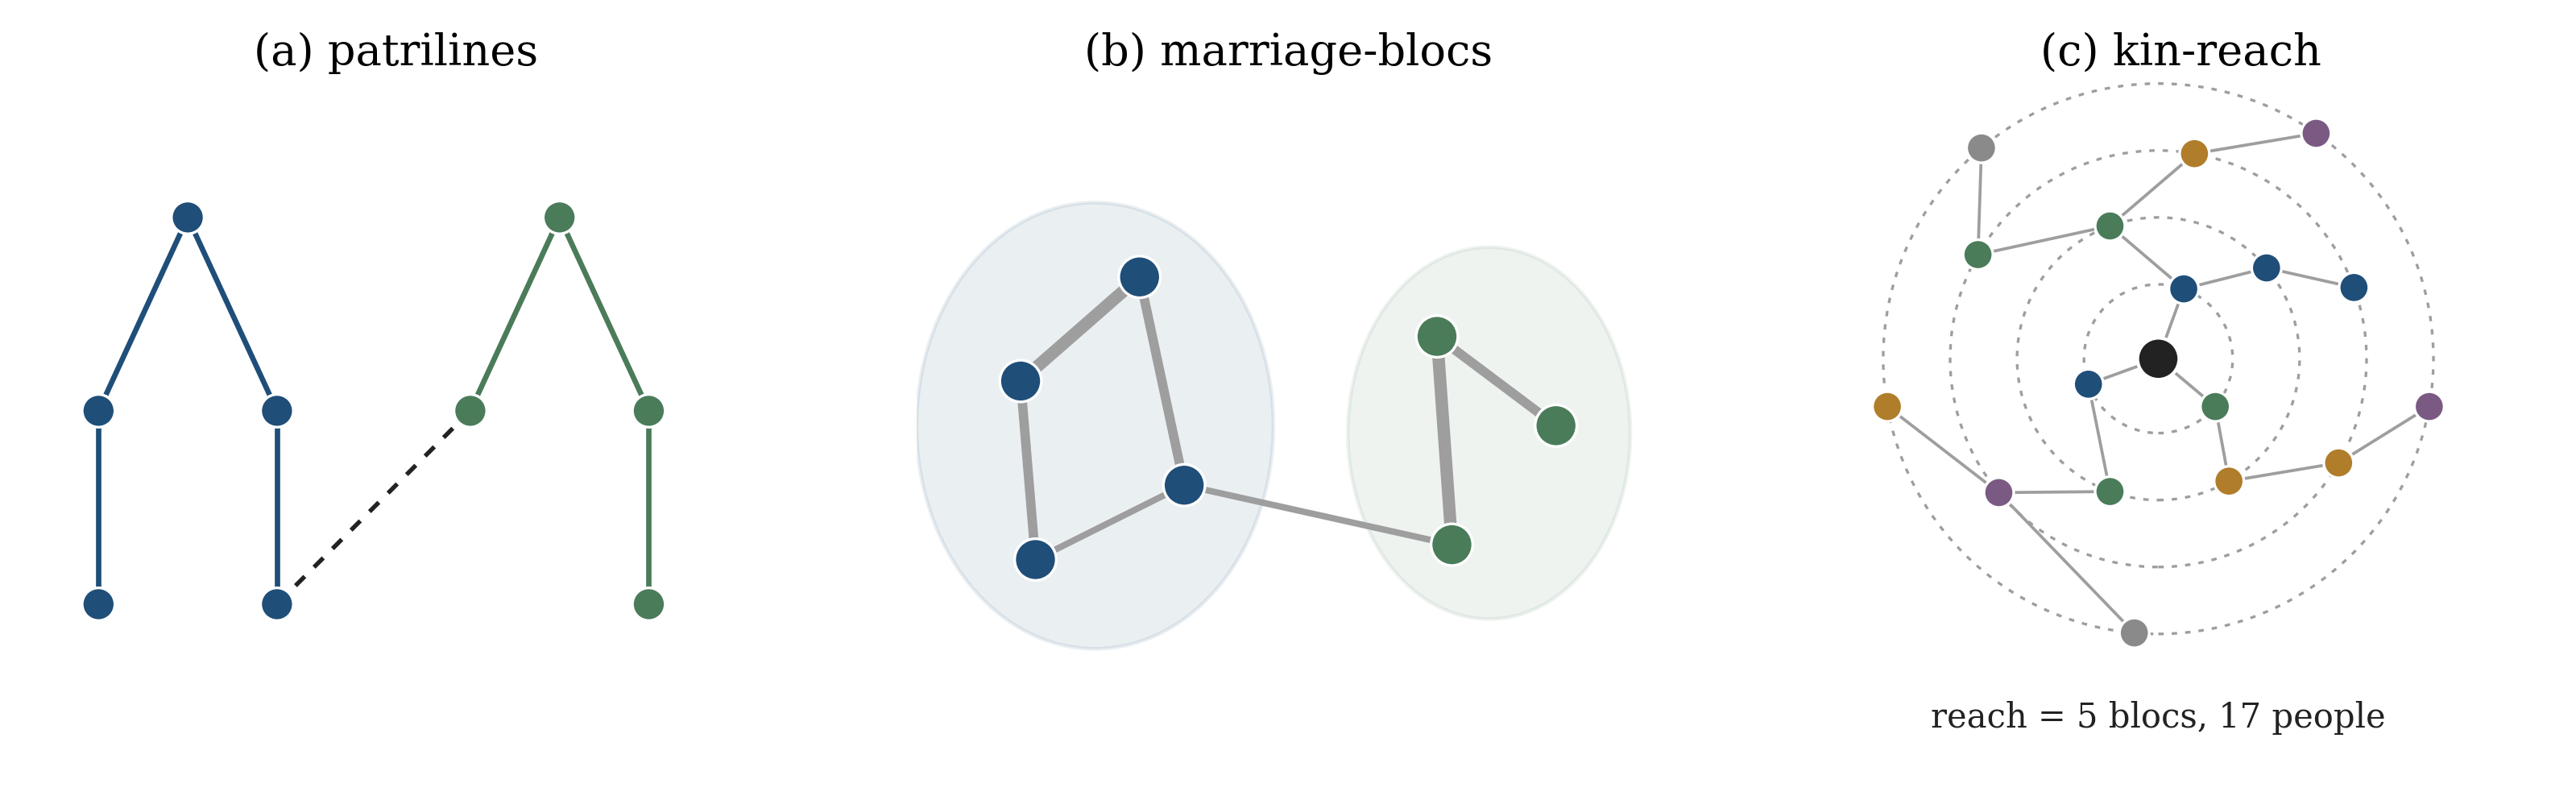
\includegraphics[width=\textwidth]{figs/fig_measure_pipeline.png}
\caption{Constructing kin-reach. (a) Patrilines are the connected components of the father--child graph. Because a daughter's children join her husband's line, marriages link patrilines without merging them. (b) Treating patrilines as nodes and marriages between them as edges, Louvain community detection groups intermarrying patrilines into marriage-blocs. (c) A noble's kin-reach is the number of distinct blocs within four kinship hops of him on the full graph.}
\label{fig:pipeline}
\end{figure}

\paragraph{Step 1: Patrilines.} I first split the genealogy into patrilines. Because a daughter's children are attached to her husband's patriline, marriages tie patrilines together but never merge them. That is, each patriline is a clean male-line descent group.

\paragraph{Step 2: Marriage-blocs.} Patrilines are too fine a partition to stand for houses. I therefore coarsen the partition. Treating each patriline as a node and placing an edge between two patrilines for each marriage between them, weighted by the number of such marriages, I apply Louvain community detection \citep{blondel_2008} to the resulting graph.\footnote{The Louvain algorithm for community detection can be thought of as a simpler version of Leiden used above. I preferred Leiden for the spanning-edge time series specifically because Leiden affords better detection of small communities; on large graphs, Louvain can merge several smaller communities into a large, badly-connected one. It turns out that in this case the worry is a non-issue: Leiden and Louvain partitions in the graphs in Figure~\ref{fig:leiden} above are functionally identical, correlating at 0.999. The motivating case for Leiden is also less important when the graph is smaller (as it is here, due to patriline coarsening). Thus, the subsequent analysis relies on the simpler Louvain algorithm. Note further that the main results are robust to alternative partitions, as discussed in Appendix~\ref{app:robust}.} The Louvain community detection algorithm is a commonly used procedure for detecting groups that have significant edge-redundancy relative to the rest of a network graph. More specifically, Louvain sorting optimizes modularity $Q$, defined as:
\begin{equation*}
  Q = \frac{1}{2m} \sum_{i=1}^{N} \sum_{j=1}^{N}
      \left[ A_{ij} - \frac{k_i k_j}{2m} \right] \delta(c_i, c_j),
  \label{eq:modularity}
\end{equation*}
where $A_{ij}$ represents the edge weight between vertices $i$ and $j$, $k_i$ and $k_j$ are the sum of the weights of edges connected to $i$ and $j$, $m$ is the sum of all edge weights in the graph, $N$ is the number of vertices, $c_i$ and $c_j$ are the communities to which $i$ and $j$ belong and $\delta$ equals $1$ if $c_i = c_j$ and zero otherwise.

The procedure returns $579$ marriage-blocs (groups of patrilines bound together by repeated intermarriage) at a modularity of $0.83$, a standard score indicating that the blocs are cleanly partitioned into distinct groups. More specifically, a modularity of $1$ denotes perfect network segmentation into groups, where a modularity of $0$ implies a graph with no topological group structure distinguishable from random connections.\footnote{Modularity $<0$ implies less structure than random; vertices systematically avoid grouping.}

\paragraph{Step 3: Reach.} A noble's kin-reach is the number of distinct marriage-blocs within four kinship hops on the full graph, counting kin born by the time of his death. A hop is one traversal of a parent-child or spouse edge, so four hops reaches, for instance, a great-great-grandparent or a spouse's sibling's child.

Figure~\ref{fig:berg} runs the same three steps on the real graph, for Adolf~VII, Count of Berg, who reappears in the papal record below. The panels show his patriline, the bloc it belongs to, and his four-hop neighborhood in turn. The last panel makes the distinction between reach and size concrete: within four hops Berg has $101$ kin, but they fall in only three blocs, so his reach is $3$.

\begin{figure}[t]
\centering
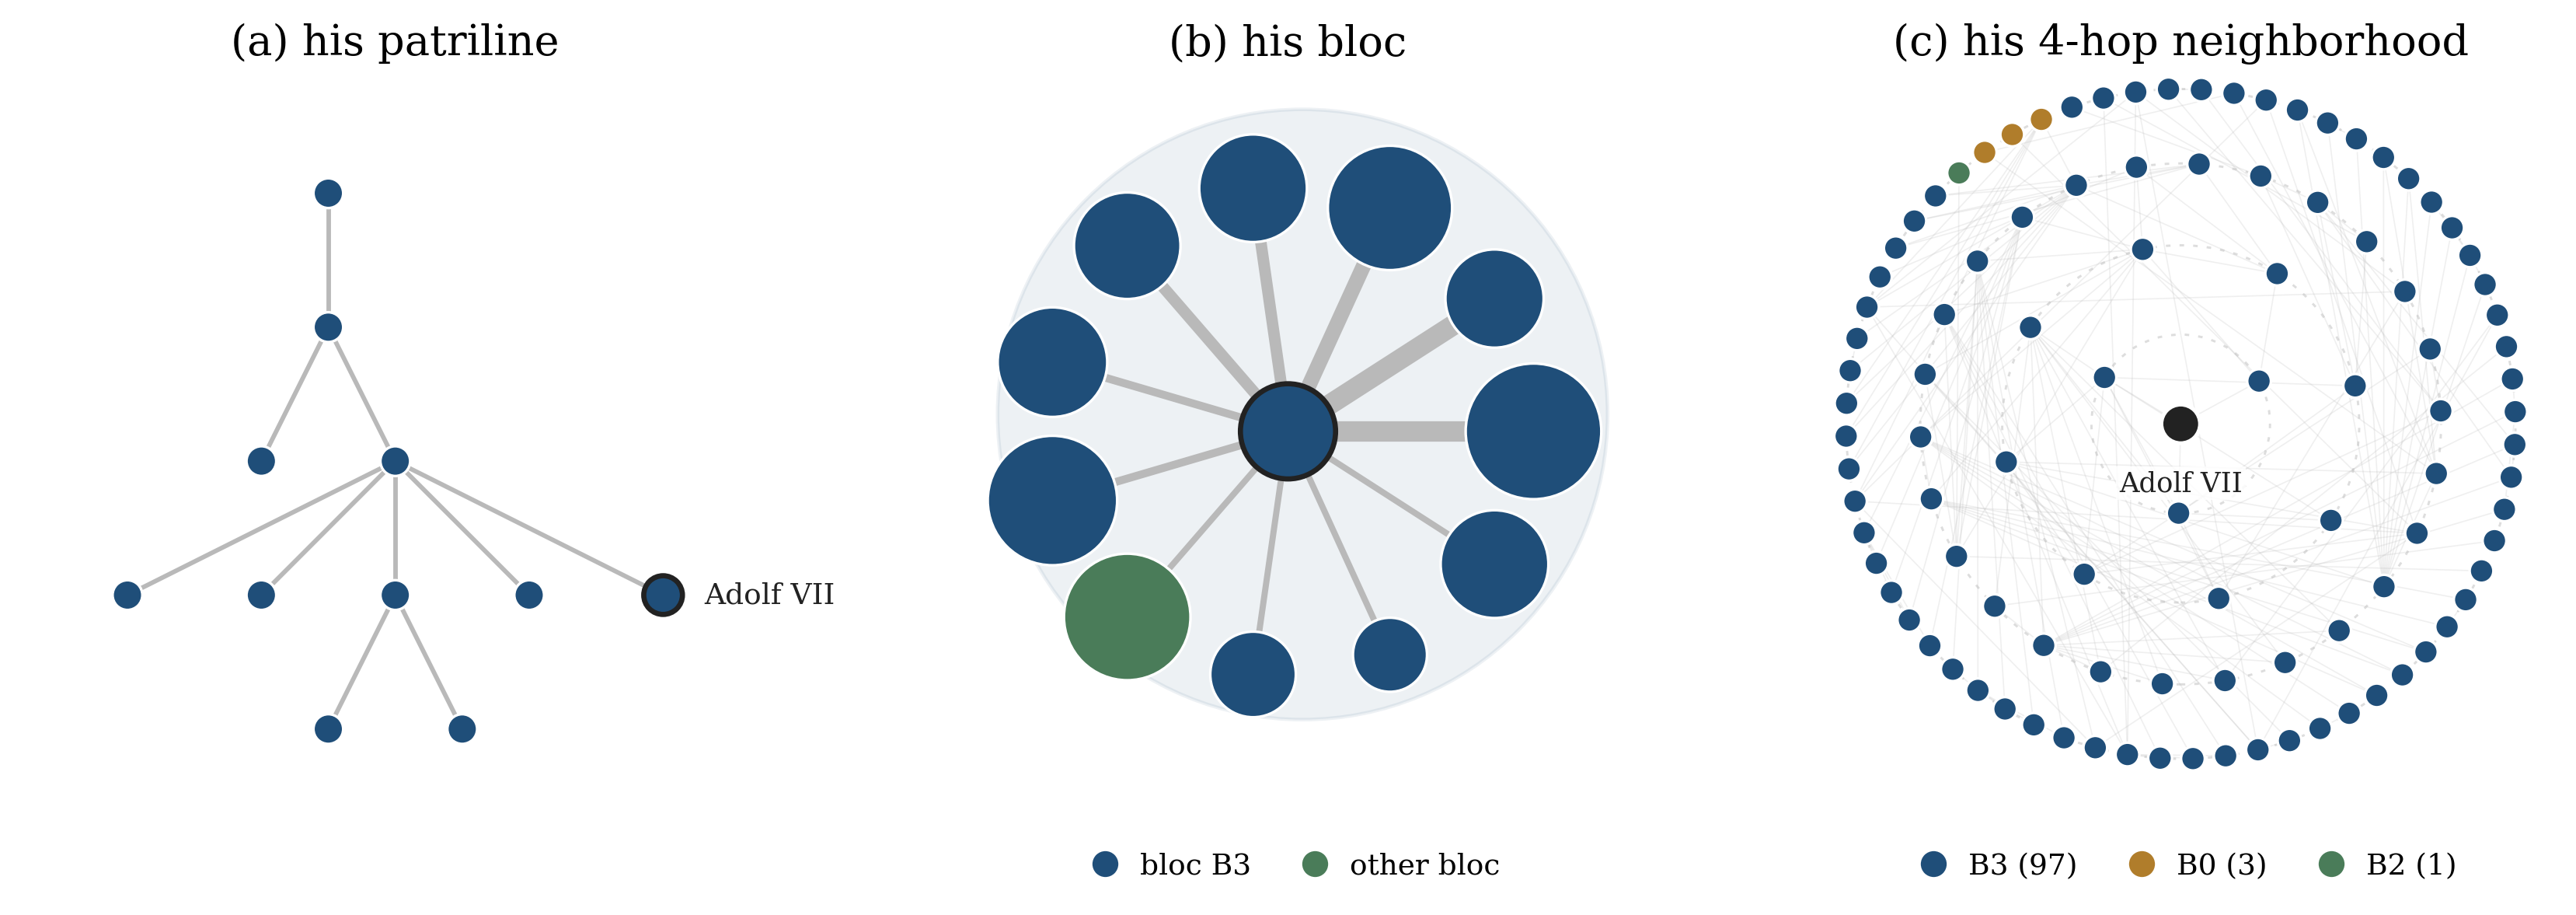
\includegraphics[width=\textwidth]{figs/fig_reach_berg.png}
\caption{The construction on real data, for Adolf~VII, Count of Berg (b.~1240, d.~1296). (a)~His patriline, the male line he descends in. (b)~His patriline (outlined) among the patrilines it marries into, which Louvain groups into bloc~B3; node area scales with patriline size and edge width with the number of marriages. (c)~His four-hop neighborhood on the full graph, $101$ people colored by bloc. They fall in only three blocs, almost all his own, so his kin-reach is $3$.}
\label{fig:berg}
\end{figure}

Coarsening to blocs allows me to cleanly distinguish between reach and the size of each noble's four-hop neighborhood. Figure~\ref{fig:reachsize} shows that size and reach are meaningfully different. Across the sample the correlation between a noble's reach and the size of his four-hop network is $0.63$; the two rise together, as they must, but a noble of given network size varies widely in how many blocs that network spans. Counted over the finer groupings the two are far harder to separate, with correlation of $0.95$ over patrilines. Thus, bloc-grouping allows me to meaningfully measure a kin-reach that is not merely a recording artifact; nobles with more recorded ancestry do not automatically have more reach.

\begin{figure}[t]
\centering
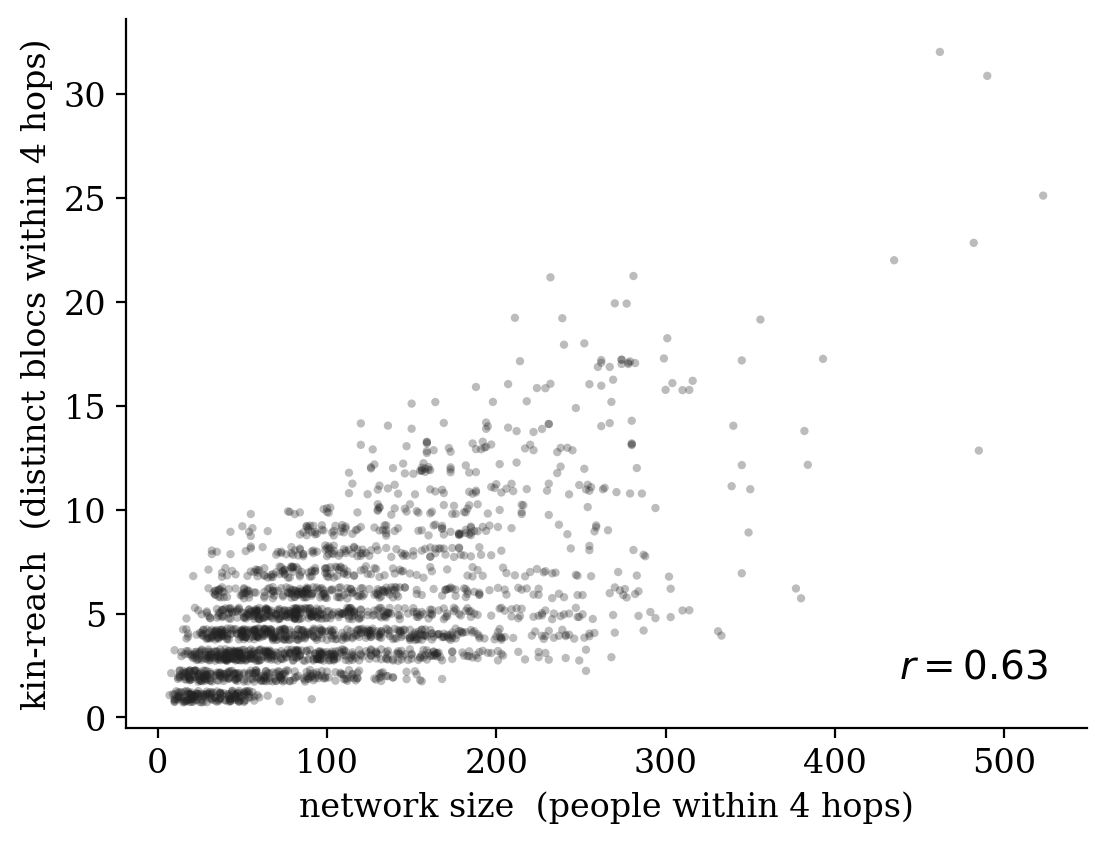
\includegraphics[width=0.66\textwidth]{figs/fig_reach_vs_size.png}
\caption{Kin-reach against network size, one point per noble in the estimation sample. Reach is the number of distinct marriage-blocs within four hops; size is the number of people.}
\label{fig:reachsize}
\end{figure}

I use four hops as the canonical boundary of reach for two independent reasons. First, reach must vary across nobles, or it identifies nothing. At short horizons almost every noble reaches only his own bloc and one or two others, and only by four hops does reach spread into a usable range (a median of four distinct blocs with a middle half of three to six). Reach must also stay distinct from size; the correlation between reach and network size climbs steadily with the horizon, from $0.57$ at three hops to $0.63$ at four and $0.75$ by six, and on finer groupings reach is size in all but name. Four hops is the first horizon that meets both requirements: wide enough that reach robustly varies across nobles, and narrow enough that it is not network size in another guise.

A second reason for preferring the four-hop radius is that textual evidence suggests that conflicts tend to occur between nobles who average a four-hop distance from one another. Below, I describe the strategy I use to match observations in \textit{The Peerage} to medieval papal communications. When I examine only those documents classified as arbitrating lay-vs.-lay territorial disputes in which at least two disputants are matched nobles in \textit{The Peerage}, I identify 221 dyads. 84 percent of these nobles are within five hops of each other, with a median of four hops and a mean of $3.7$. Thus, empirically, four hops seems to be the relevant distance -- nobles that you might conflict with live about four hops away from you.

In the following analysis, the estimates themselves hold at hops three-to-five and become indistinguishable from zero at six hops. (Appendix~\ref{app:robust}).

For the purposes of the following analysis, I compute the kin-reach of a sample of $2{,}195$ male nobles whose lifespans overlap 1100--1300 and whose genealogies are sufficiently well-attested that they have ancestors in the 900s.\footnote{More specifically, these are the male nobles who were assigned dynasties in Section~\ref{sub:facts} above. The dynasty labels here have no significance; I'm simply sorting nobles based on the depth of their pedigree.} This restricts the analysis to only the most historically important nobles and helps to mitigate concerns about variance in genealogical completeness.

\begin{figure}[t]
\centering
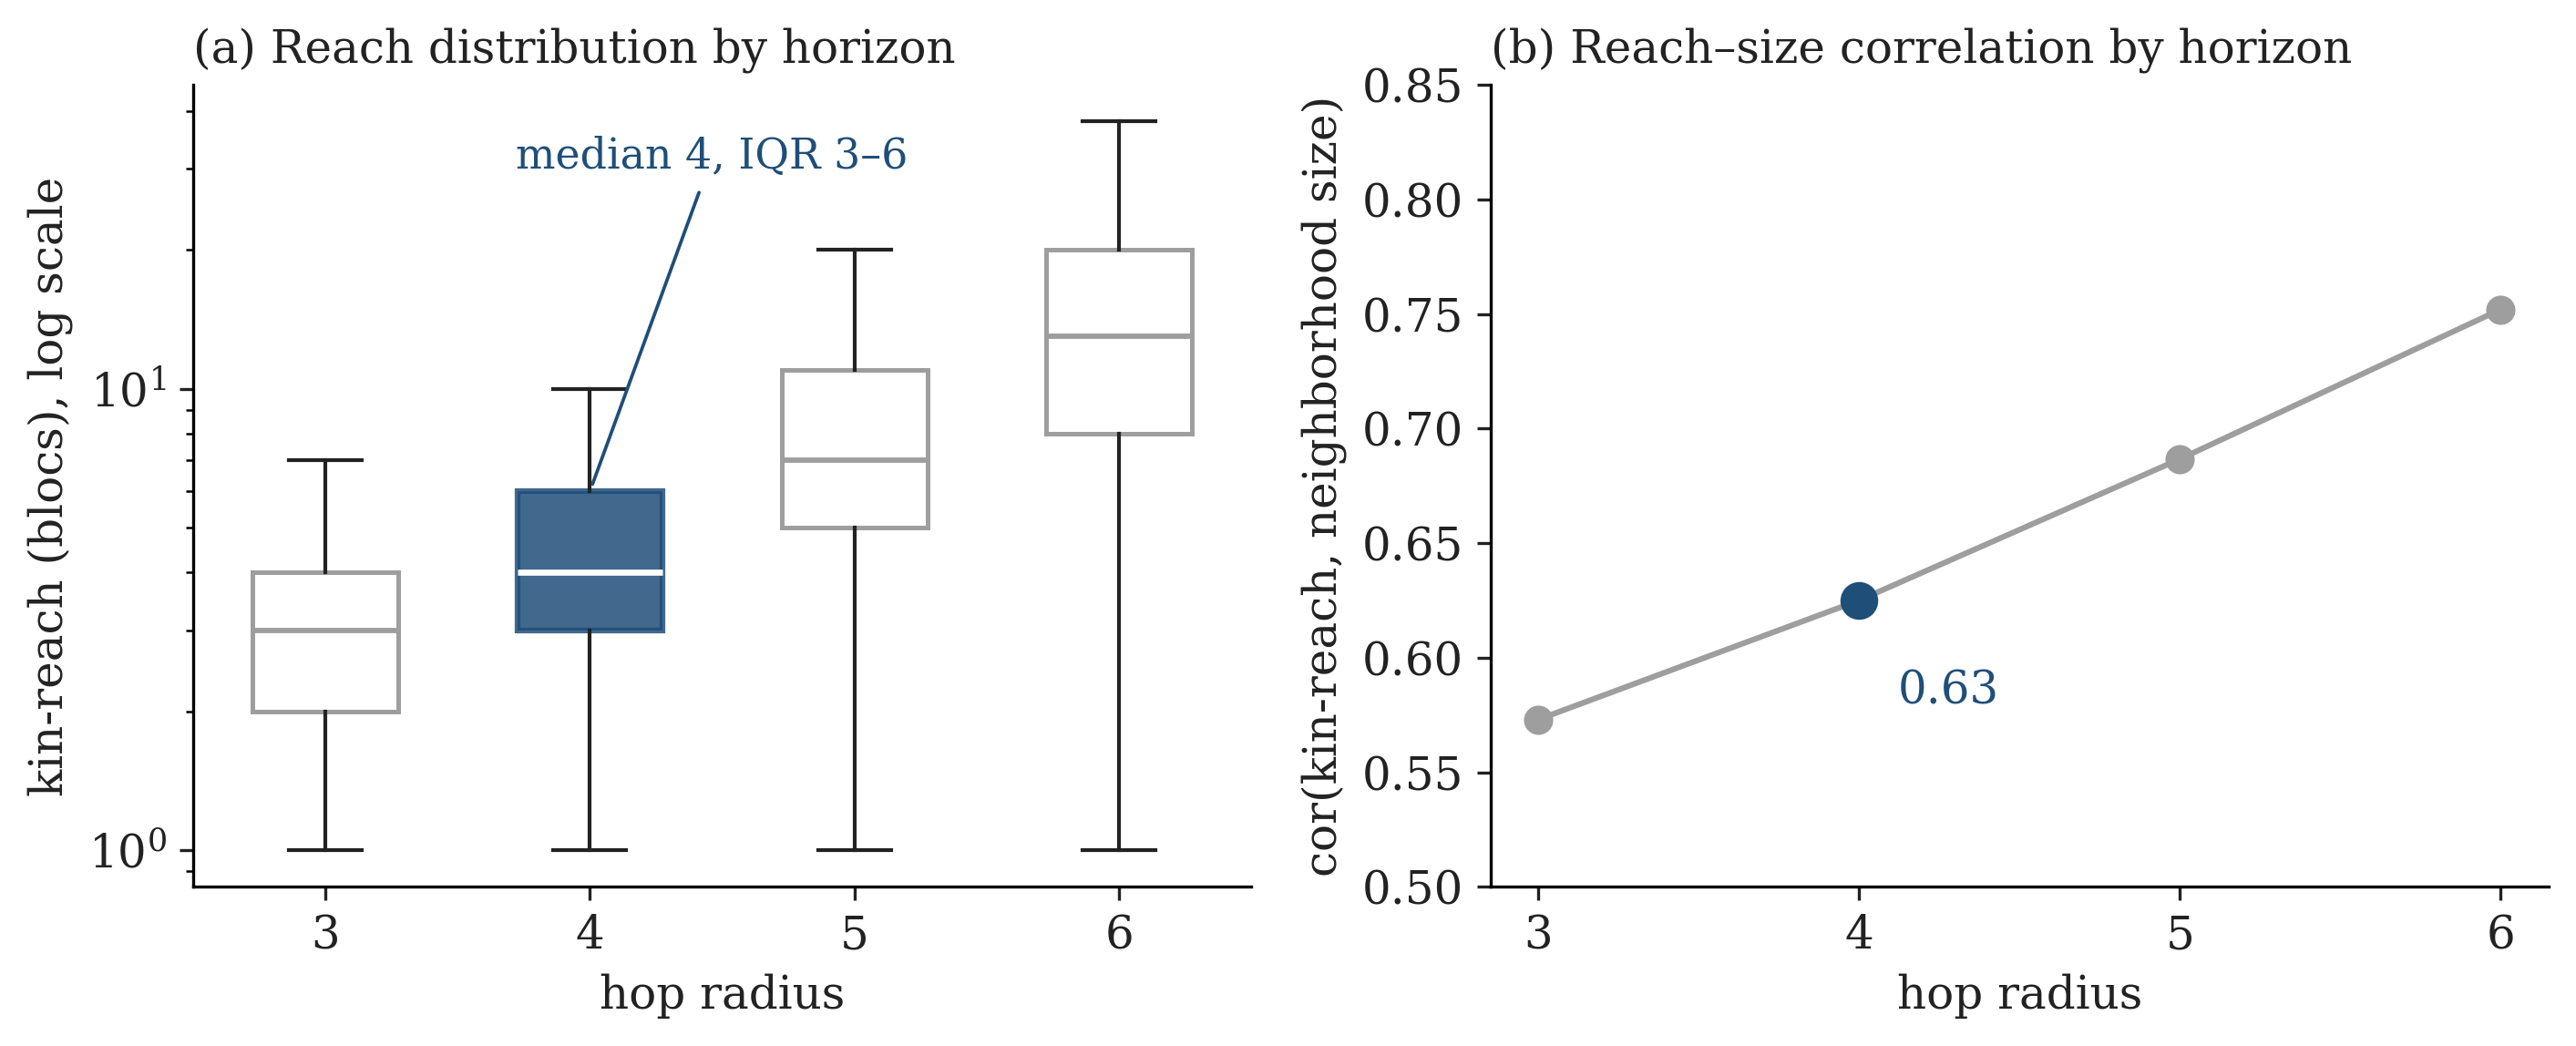
\includegraphics[width=\textwidth]{figs/fig_horizon.png}
\caption{(a) The distribution of kin-reach across nobles in the estimation sample, by the number of hops used to define it. (b) The correlation between kin-reach and raw network size, by horizon.}
\label{fig:horizon}
\end{figure}

\subsection{Papal arbitration}

No large-scale repository of high medieval ecclesiastical court proceedings exists. Surviving records are scattered across European archives, largely undigitized, and unsystematic before the late thirteenth century. For the sample I study (historically important nobility), however, the papal correspondence is a very close substitute for court records. The model predicts demand for arbitration. At the highest level of politics, arbitration was often provided directly by papal decree, or indirectly through papal instructions to particular legal representatives.

The outcome variable is a noble's appearance in papal documents related to territorial disputes, constructed as follows. First, I match persons to letters with a large language model (LLM; Claude Sonnet 4.6) run in closed-set mode. For each letter, the model receives the letter's text and a shortlist of nobles whose lifespans overlap the letter's date and whose partial name strings occur in the letter. The model returns those shortlisted nobles who actually appear in the text, each with a stated confidence (low, medium, or high). The model found $6{,}407$ high-confidence noble-letter matches across $521$ nobles and $4{,}536$ letters. Details on validation are available in Appendix~\ref{app:data}. The key fact is that two independent audits by the researcher and a research assistant, respectively, each of a disjoint random sample of $100$ documents with high-confidence matches, show that across the $200$ documents, $95.4\%$ of matches were correct.\footnote{More specifically, the researcher found that  $93/97$ matches were correct, with three unsure removed from the sample, while the assistant found that $93/98$ matches were correct, with two unsure removed from the sample. Pooling precision by terciles of matched-noble's reach gives $0.935$, $0.962$, and $0.978$ respectively. Precision thus grows slightly across terciles, which biases subsequent results slightly downward. That is, this fact implies that the estimates in my regression models are conservative. All rejected matches are same-name disambiguation errors, usually between adjacent members of a dynasty (e.g. Charles I of Anjou was confused by the LLM with his son Charles II in a letter sent in 1285, the year of I's passing and II's succession).}

To distinguish the resolution of disputes from other kinds of documentary engagement, I submit each matched letter to another instance of the LLM and ask it to answer two questions. First, it records whether the letter concerns a live dispute (as opposed to a one-sided grant or confirmation or a passing mention). Second, it assigns the letter to exactly one of eight subject domains. See Figure~\ref{fig:codedoc} for an example.

\begin{figure}[t]
\centering
\fbox{\begin{minipage}{0.90\textwidth}
\footnotesize
\textbf{APOSCRIPTA no.~160468} \hfill Honorius~IV, 1286\\[3pt]
\textit{Source summary.} ``Le pape Honorius institue des arbitres pour juger le diff\'erend survenu entre la ville d'Anvers et Adolphe comte de Berghe.''\\[3pt]
\textit{Matched noble.} Adolf~VII von Berg, located in \emph{The Peerage}. The opposing party is the city of Antwerp.\\[5pt]
\begin{tabular}{@{}p{5.2cm}l@{}}
\toprule
live dispute? & yes\\
is the matched noble a principal? & yes\\
domain & secular-territorial\\
\bottomrule
\end{tabular}
\end{minipage}}
\caption{A coded letter. The pope names arbiters to settle a territorial quarrel between the Count of Berg and the city of Antwerp. The letter is a live dispute in the secular-territorial domain. The matched noble is one of its principals.}
\label{fig:codedoc}
\end{figure}

Figure~\ref{fig:domains} reports summary statistics on the matched letters. Note that letters with the subject ``secular-territorial'' are also the largest source of disputes.

\begin{figure}[t]
\centering
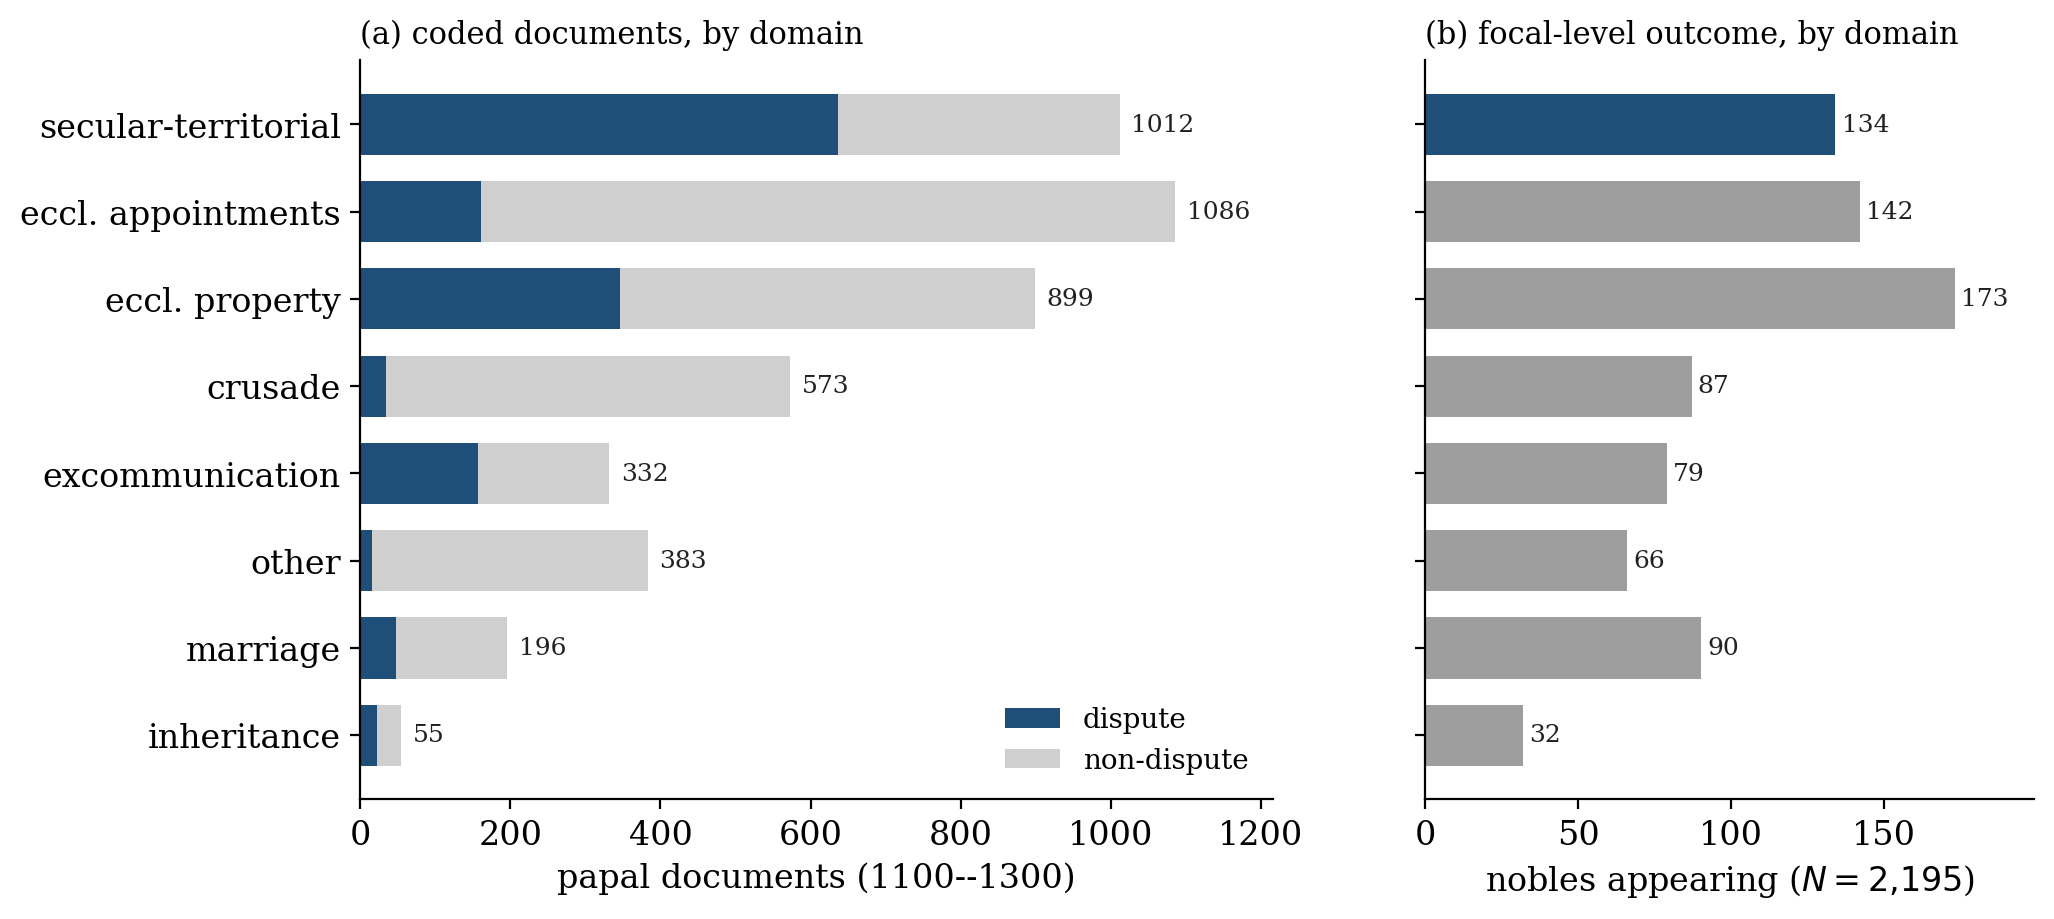
\includegraphics[width=\textwidth]{figs/fig_domain_distribution.png}
\caption{The coded outcome. (a) Papal letters matched to sampled nobles, by domain, split into live disputes and other business. (b) The number of sampled nobles ($N=2{,}195$) who appear in at least one letter of each domain.}
\label{fig:domains}
\end{figure}

I test the LLM subject-coding's reproducibility against an independent second coding of a subset of $2{,}000$ letters, produced by a separate model pass under the same instructions. Table~\ref{tab:kappa} reports the agreement. The dispute axis and the eight-way domain agree at Cohen's $\kappa$ of $0.70$ and $0.68$. For the assignment to ``secular-territorial" in particular, the two coders agree at a raw rate of $88.5$ percent, with Cohen's $\kappa$ of 0.62. Where the models disagreed, the alternative categories were most frequently the ``ecclesiastical property" and ``other" categories.

\begin{table}[t]
\centering
\caption{Inter-coder agreement between two independent codings of the same letters.}
\label{tab:kappa}
\begin{tabular}{lccc}
\toprule
Axis & Agreement & Cohen's $\kappa$ & $n$ \\
\midrule
Live dispute (yes/no) & 88.3\% & 0.70 & 2{,}000 \\
Domain (eight-way) & 73.3\% & 0.68 & 2{,}000 \\
Parties to the dispute & 84.8\% & 0.72 & 407 \\
Matched noble a principal & 90.9\% & 0.80 & 407 \\
\bottomrule
\end{tabular}
\end{table}

For each noble in the sample I count the letters in each domain in which he appears over $[1100,1300]$. I use the count in logs, $\log(1+n)$. Of the $2{,}195$ nobles in the sample, $297$ appear in at least one letter. The subsequent analysis shows that a noble's kin-reach causally raises counts in the predicted domains.

% ===== END sections/measure_section_7_1_26 =====



% ===== BEGIN sections/results_section_7_1_26 =====
\section{Results}
\label{sec:results}

I test the theory's predictions in turn: that a noble's kin-reach raises his demand for arbitration and that the demand is contagious across the kin network.

\subsection{Kin-reach and the demand for arbitration}
\label{sub:forward}

The model's first prediction is that broader kin-reach raises a noble's engagement in the papacy's dispute-resolution business, measured by the count of dated papal dispute letters in which he appears. Reach, though, is partly a choice of the noble. Relatively exogamous nobles are likely to differ from those that are not in ambition, importance, and documentary survival, all of which also may raise their appearances in APOSCRIPTA documents. Ordinary least squares confounds these channels. I therefore instrument.

The instrument is the focal noble's mother's kin-reach, counted before his birth: the number of blocs within four hops of his mother among kin born before he was (Section~\ref{sec:measurement}). Because a mother's prior network mechanically builds much of her son's, the instrument predicts reach exceptionally well (first-stage $F=339$). Because a son's court appearances cannot shape his mother's network before he existed, the instrument rules out reverse causality.

The remaining concern is exclusion. That is, the inherited network must affect the noble's documentary appearances only through his own reach. There are a number of threats here. First, a noble's mother's reach might drive her own marriage decisions, therefore affecting the outcome variable directly through properties of her husband. The major concern here is that mothers with high reach give their husbands that reach, and therefore cause their husbands to appear in papal documents; her sons then mechanically inherit these disputes. I correct this bias by controlling for the number of papal documents in which a noble's father appears. Similarly, a noble could inherit conflicts through his mother from his maternal grandfather; I control for the grandfather's documentary footprint as well. Effects could plausibly be driven by recording asymmetries; a noble with a larger number of kinsmen within four hops mechanically can be expected to have higher reach. The worry, then, is that a noble's documentary footprint is correlated with the relative completeness of his family's dynastic records, giving an artificial result; I therefore control for mother's, father's, and maternal grandfather's counts of nobles within four hops. Similarly, I control for each of the mother's, father's, and maternal grandfather's degree (number of edges). Most of the nobles have titled ranks determinable from regex matching in their names (for instance, \textit{comte} for French counts). I control for title-rank using indicator variables. In order to cleanly isolate maternally-inherited reach, I control for the grandfather's reach and for the father's bloc-increment (the extra blocs he adds over the mother's reach); using the increment prevents the control from becoming nearly collinear with the instrument. Each of these variables is computed for a graph that includes only those born before the focal noble. Finally, I include death-decade and marriage-bloc fixed effects, as well as an indicator for the focal noble's own title rank.

There is one obvious exclusion worry remaining. It may be the case that mothers with high reach are merely more conflict prone, or belong to more conflict-prone families. Rather than create arbitration, reach simply creates conflict, which happens to be mentioned in papal letters. This worry is unlikely to be very serious: as I explain in more detail below, the effect of reach on appearances in papal documents is concentrated among nobles who can be independently identified as conflict-prone; and conflict proneness is almost perfectly orthogonal to reach after including the battery of controls listed above. 

Figure~\ref{fig:dag} shows the exclusion worries and the controls that address them. I specify the exact model below.

\begin{figure}[t]
\centering
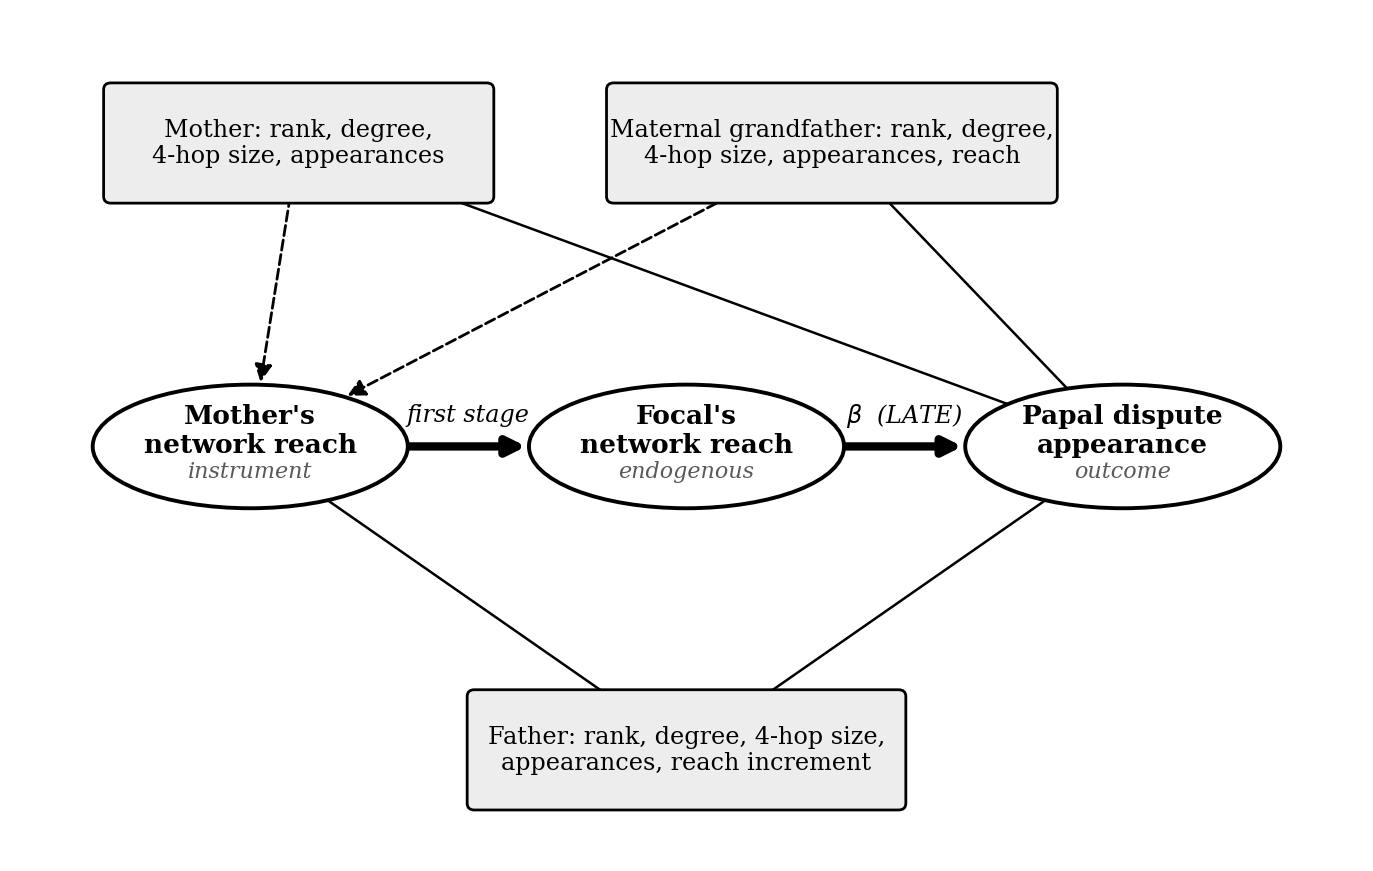
\includegraphics[width=0.9\textwidth]{figs/fig_iv_dag.png}
\caption{The mother's pre-natal reach (instrument) shifts the focal's reach (treatment), which raises his appearance in the papacy's dispute business (outcome). The mother's, father's, and maternal grandfather's rank, connectedness, and papal activity are controlled confounding paths.}
\label{fig:dag}
\end{figure}

\begin{align}
\text{(second stage)}\qquad
\log\!\bigl(1+Y_i^{c}\bigr) &= \beta^{c}\,\widehat{R}_{i}
  + \mathbf{X}_i'\boldsymbol{\gamma} + \mu_{b(i)} + \lambda_{t(i)} + \varepsilon_i,\\[2pt]
\text{(first stage)}\qquad
R_{i} &= \pi\, R^{M}_{i}
  + \mathbf{X}_i'\boldsymbol{\delta} + \mu_{b(i)} + \lambda_{t(i)} + \nu_i,
\end{align}

\begin{itemize}
\item $Y_i^{c}$ --- the number of papal letters in domain $c$, issued in $[1100,1300]$,
      in which noble $i$ appears.
\item $R_i$ --- kin-reach: distinct marriage-blocs within four hops of $i$ on the
      full kinship graph, among kin born by $i$'s death; endogenous.
\item $R^{M}_i$ --- the mother's pre-natal kin-reach, computed on the same graph
      over kin born before $i$'s birth; the excluded instrument.
\item $\mu_{b(i)}$, $\lambda_{t(i)}$ --- marriage-bloc and death-decade fixed effects.
\item $\mathbf{X}_i$ --- focal title-rank fixed effects;
      for each ancestor $a \in \{M, F, M\!G\!F\}$: title-rank fixed effects,
      $\log(1+N_a)$ pre-natal network size within four hops,
      $\log(1+\mathrm{deg}_a)$ pre-natal degree, and $\log(1+A_a)$ in-window papal
      appearances; and the maternal grandfather's reach $R^{M\!G\!F}_i$ and the father's additional reach (blocs reached in father's 4-hop not reached in mother's).
\end{itemize}

The regression sample consists of $2{,}195$ male nobles whose lifespans overlap 1100--1300 and whose maternal network instruments are computable, drawn from the pedigree-based sampling frame described in Section~\ref{sec:measurement} and Appendix~\ref{app:data}. Summary statistics for the sample are reported in Table~\ref{tab:summary_sample}.


% ===== BEGIN tables/tab_summary_sample =====
\begin{table}[!t]
\centering
\caption{Summary statistics: the estimation sample.}
\label{tab:summary_sample}
{\small
\begin{tabular}{lccccc}
\toprule
 & Mean & SD & Median & \multicolumn{2}{c}{Mean by appearance} \\
\cmidrule(lr){5-6}
 & & & & Appearers & Others \\
\midrule
\multicolumn{6}{l}{\textit{Panel A: vitals}} \\
Birth year & 1202 & 71 & 1217 & 1190 & 1204 \\
Death year & 1252 & 70 & 1264 & 1241 & 1254 \\
Lifespan (years) & 49.7 & 16.6 & 53.0 & 51.0 & 49.5 \\
Titled (rank $\geq$ 1) & 51\% & -- & -- & 82\% & 46\% \\
Royal or imperial (rank $\geq$ 4) & 8\% & -- & -- & 31\% & 4\% \\
\addlinespace
\multicolumn{6}{l}{\textit{Panel B: kinship network}} \\
Kin-reach (blocs within 4 hops) & 5.12 & 3.42 & 4.00 & 6.21 & 4.95 \\
Network size (persons within 4 hops) & 106.4 & 71.6 & 90.0 & 173.3 & 95.9 \\
Degree & 4.41 & 2.97 & 4.00 & 6.88 & 4.02 \\
Mother's pre-natal reach (instrument) & 4.75 & 3.55 & 4.00 & 5.38 & 4.65 \\
Mother's pre-natal network size & 82.0 & 64.1 & 67.0 & 109.7 & 77.7 \\
Father's pre-natal reach & 5.03 & 3.78 & 4.00 & 5.67 & 4.93 \\
Maternal grandfather's pre-natal reach & 5.79 & 4.82 & 5.00 & 6.26 & 5.71 \\
\addlinespace
\multicolumn{6}{l}{\textit{Panel C: papal appearances, 1100--1300}} \\
 & Share $>0$ & Mean & \multicolumn{3}{c}{Among those appearing} \\
\cmidrule(lr){4-6}
 & & & Median & P90 & Max \\
Total appearances & 14\% & 2.42 & 3 & 31 & 858 \\
Secular-territorial appearances & 6\% & 0.70 & 2 & 28 & 275 \\
Dispute appearances & 9\% & 0.84 & 2 & 22 & 318 \\
\midrule
\multicolumn{6}{p{0.92\textwidth}}{\footnotesize \textit{Notes:} $N=2,195$ male nobles across 38 marriage-blocs; 297 appear in at least one letter. Reach and size are computed on the full kinship graph over kin born by the focal's death; ancestors' values over kin born before the focal's birth. First-stage $F = 339$; cor(reach, size) $= 0.63$. The father and maternal grandfather pre-natal reach rows have smaller samples ($N=2{,}189$ and $N=1{,}856$, respectively) of only those who have reach $>0$. The 858-appearance noble is Frederick II Hohenstaufen; results survive his omission (see robustness appendix).} \\
\bottomrule
\end{tabular}
}
\end{table}
% ===== END tables/tab_summary_sample =====



% ===== BEGIN tables/tab_domains =====
\begin{table}[t]
\centering
\caption{Kin-reach and papal appearance, by subject domain. Each row is a separate 2SLS regression of $\log(1+\text{appearances})$ in that domain on kin-reach instrumented by pre-natal maternal reach. $N=2,195$; $38$ blocs; first-stage $F=339$. $p$ is bloc-clustered; $p_{\text{2-way}}$ clusters on bloc and decade. The last column indicates the number of nobles with at least one appearance in the specified domain.}
\label{tab:forward}
\begin{tabular}{lccccc}
\toprule
Domain & $\beta$ & SE & $p$ & $p_{\text{2-way}}$ & $n>0$ \\
\midrule
\textbf{Secular-territorial} & \textbf{0.033} & 0.005 & $<$0.001 & \textbf{0.005} & 134 \\
Ecclesiastical appointments & 0.022 & 0.007 & 0.002 & 0.091 & 142 \\
Crusade & 0.022 & 0.006 & 0.002 & 0.069 & 87 \\
Other (heresy, diplomacy) & 0.015 & 0.002 & $<$0.001 & 0.057 & 66 \\
Excommunication & 0.014 & 0.007 & 0.061 & 0.072 & 79 \\
Ecclesiastical property & 0.012 & 0.009 & 0.208 & 0.335 & 173 \\
Inheritance & 0.003 & 0.004 & 0.418 & 0.550 & 32 \\
Marriage & -0.001 & 0.002 & 0.825 & 0.909 & 90 \\
\midrule
All documents & 0.032 & 0.009 & $<$0.001 & 0.122 & 297 \\
\bottomrule
\end{tabular}
\end{table}

% ===== END tables/tab_domains =====


Table~\ref{tab:forward} reports one instrumented regression per subject domain, on the sample of $2{,}195$ male nobles across $38$ blocs. The effect clearly concentrates in \emph{secular-territorial} documents, where each additional bloc within a noble's reach raises his appearances by about three percent ($\beta=0.033$). Note further that secular-territorial is the one domain that remains significant given two-way clustering by bloc and decade ($p=0.005$).

Because thirty-eight blocs is plausibly few for cluster asymptotics, I also permute the instrument across nobles within bloc-by-decade cells (999 draws). The observed reduced form in this case lies eight standard deviations outside the placebo distribution ($p=0.001$). Permuting at the mother level instead, so that siblings always share a value, still leaves it five to six standard deviations out ($p = 0.001$). A restricted wild-cluster bootstrap of the reduced form of the outcome on the instrument is highly conservative, given that a single bloc holds $29$ percent of the sample. It yields $p=0.07$--$0.15$ depending on weighting and on whether that largest bloc is included. A control-function Poisson model has similarly inflated standard errors but a near identical coefficient.\footnote{And interestingly, in the Poisson model, reach reduces marriage letters. I take this as nicely suggestive of correspondence between the genealogy and the law; nobles with high reach did not need dispensations to marry within prohibited degrees.} Appendix~\ref{app:robust} reports the full battery. Conversely, reclustering at the patriline level and replacing bloc fixed effects with patriline and decade fixed effects (so that identification is within sets of brothers or cousins) nearly doubles the secular-territorial effect coefficient ($\beta = .059$) but moves significance to marginal ($p = .097$), while preserving effect size and significance ordering across domains.

Reach could merely proxy importance, driving general prominence in papal communications: nobles with well-attested genealogies might be more likely to communicate with the pope. The effect's concentration in territorial letters ameliorates this worry, but I test it formally by controlling for non-territorial papal activity. In this case, the territorial effect is $0.02$, still two-way robust ($p_{\text{2-way}}=0.003$). And note that this is a bad control which opens a downwardly biased collider path and therefore the estimate is conservative. Additionally, including an indicator for heiress mothers (defined as mothers whose patrilines have no surviving men at the time of the focal noble's birth) leaves the estimate at 0.0326 ($F=354$), while the indicator's estimate is zero, again pushing against generic prominence -- nobles who inherit high reach from their mothers are not also somehow inheriting wealth that then converts into papal communications.

The territorial effect is not driven by any one bloc or observation. Dropping each of the $38$ blocs in turn leaves it significant in every case, with the coefficient between $0.029$ and $0.037$. Dropping the single largest bloc, which alone supplies two-fifths of the territorial appearances, lowers the coefficient only to $0.031$. Dropping Frederick~II Hohenstaufen, the single most-documented noble in the sample, leaves it at $0.033$ ($p_{\text{2-way}}=0.004$). The effect similarly persists when reach is computed at three and five hop horizons.

To corroborate the conflict-resolution channel, I identify a subset of nobles as conflict-prone. This subset of nobles consists of nobles who have at least one of the following: a living maternal great-uncle at birth, a male sororal cousin but no maternal uncles, or a mother with at least two husbands. One would \textit{prima facie} expect disputes to concentrate among these nobles; these are cases that generate multiple ambiguous, contestable claims to various rights. After the battery of controls, the partial correlation of conflict-proneness with the instrument is $-0.003$. Running the above regressions on the two subsamples -- the conflict-prone and the rest -- reveals that the effect of reach on appearances in secular-territorial documents is almost entirely concentrated among the conflict prone ($\beta = 0.053$, $p_{\text{2-way}} = 0.0008$) and that the effect of reach on appearances in any category for those outside of the conflict-prone subset is zero. Further, within the conflict prone group, the placebo categories remain null; smaller effects ($\beta \approx 0.02$) are detectable for excommunication and ecclesiastical property only, while appointments and crusade sit just outside two-way significance, and marriage and inheritance remain null. An interaction-variable model shows that the interaction of reach and conflict-prone predicts secular-territorial appearances ($\beta = 0.034$, $p_{\text{2-way}} = 0.01$), while the reach by itself predicts nothing and conflict-proneness in fact \textit{negatively} predicts appearances (I take this latter fact to be suggestive evidence of substitution -- nobles move from the battlefield to arbitration -- though it is worth noting that this particular coefficient is somewhat fragile, as discussed in Appendix~\ref{app:robust}).

Full results for these regressions and other robustness checks are reported in Appendix~\ref{app:robust}.

Endogeneity concerns prevent me from taking the conflict-prone decomposition as causally estimated. Rather, the decomposition reveals descriptive heterogeneity that strengthens the causal case for the estimations in Table~\ref{tab:forward}. The effect is concentrated among the conflict prone; this pushes strongly against a generic prominence story where more important nobles simply happen to have more recorded genealogies and more communications with the pope. Nobles with more recorded genealogies do not, in fact, have more communications with the pope; they only do if they are conflict prone. It also pushes strongly against an alternative theory where the EMFP simply created more conflicts, because the reach effect exists only among groups that we have independent reasons to think are already conflict prone; and their conflict-proneness is orthogonal to reach. This fact closes off the remaining exclusion worry opened above. Finally, the decomposition effectively mitigates concerns about reach-stratified recall. The LLM-matching was audited for accuracy (false positives), but not recall (false negatives). If recall improved, for some reason, with reach -- if there were fewer missed matches among nobles with high reach -- the result would be produced mechanically. But it seems deeply implausible to think that recall would improve with reach \textit{only} for those nobles who we have independent reason to think are conflict-prone.

\subsection{The peer channel}
\label{sub:network}

The theory's second prediction is that the demand for arbitration spreads through the kin network through two mechanisms. First, arbitration is useful only against counterparties who will submit to arbitration (arbitration is a network good). Second, a noble's peers' exogamy makes every alliance around him less reliable, raising the riskiness of force whether or not any peer ever arbitrates (ambient risk). The obvious instrument for peer court use -- some measure of peer network structure -- therefore fails its exclusion restriction by the model's own logic. So I estimate the composite peer effect in reduced form.

I build two peer variables. The first is \emph{peer breadth}. For each noble's pre-natal kin within four hops, I take the average count of distinct marriage-blocs among each kinsman's own earlier-born neighbors (that is, one-hop connections). Breadth thus measures the ambient risk around a noble. Importantly, breadth is distinct from reach: the maternal reach instrument correlates with pre-natal breadth at 0.52 (and the partial correlation falls to 0.22 when conditioning on the battery of controls above).\footnote{Some readers will worry that breadth then appears to be an uncontrolled threat to exclusion for the IV above. The short response is that the IV estimates the composite effect of exogamy in the noble's neighborhood, his own and others'; my theory requires that there be an effect of exogamy, identified above, and that some of that effect be a peer effect, identified in this section. Conditioning on breadth opens a collider path, so the only causal effect I can identify is the composite. However, for those who are curious, the secular-territorial coefficient when controlling for breadth is $0.029$; it is still the only two-way significant subject, and the effect size and significance ordering across subjects is preserved. If breadth merely under-measures the ambient channel, $0.029$ is an upper bound on the non-peer effect and the absorbed $0.004$ a lower bound on the peer share. If breadth instead over-controls (which it might, since it is partly built from the mother's own pre-natal marriages and correlates with own reach at $0.49$) the non-peer effect exceeds $0.029$. Under either reading, the composite's existence, magnitude, and domain specificity are untouched.} The second is the \emph{peer arbitration share}: the share of those same kin who appear in a secular-territorial letter dated before the focal's birth. Note further that the two peer (breadth and arbitration share) variables are nearly orthogonal ($r=0.09$). Figure~\ref{fig:peer_construction} works through the construction for a noble in the dataset. Table~\ref{tab:summary_peers} reports summary statistics.

\begin{figure}[t]
\centering
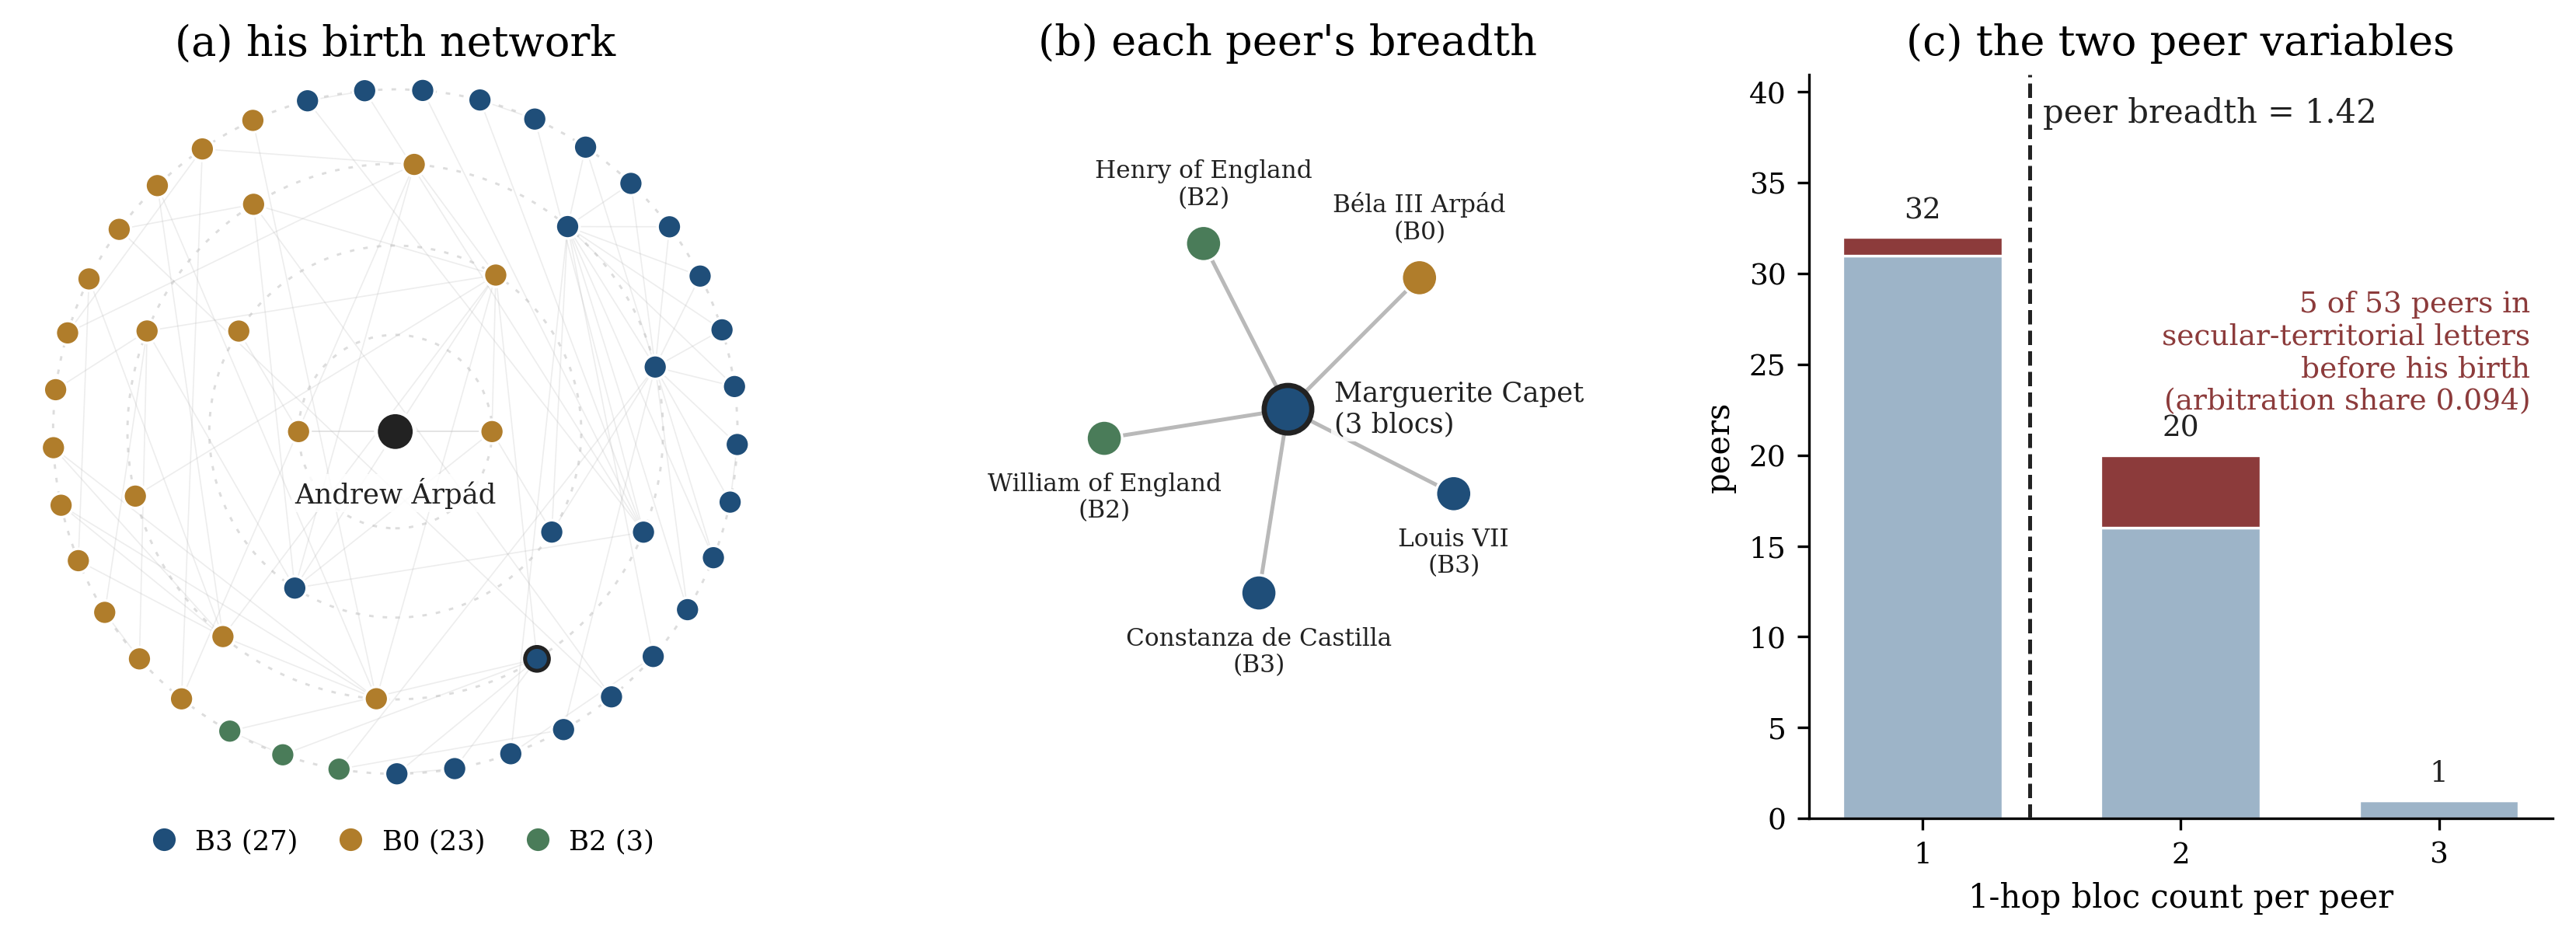
\includegraphics[width=\textwidth]{figs/fig_peer_triptych.png}
\caption{Constructing the peer variables, for Andrew \'Arp\'ad, son of King Andrew II of Hungary (b.~1205). (a)~His birth network: the $53$ kin within four hops reached through people born before him, colored by marriage-bloc. (b)~Each peer's breadth is that peer's count of distinct blocs among his or her own pre-1205 neighbors; Marguerite Capet reaches three, through Henry and William of England, B\'ela III of Hungary, Louis VII, and Constance of Castile. (c)~Averaging over the $53$ peers gives Andrew's peer breadth ($1.42$); the five peers who appear in secular-territorial letters before his birth --- his father Andrew II, his uncle King Emeric, Ottokar I of Bohemia, Pierre I Capet, and Constance of Aragon --- give his peer arbitration share ($0.094$).}
\label{fig:peer_construction}
\end{figure}


% ===== BEGIN tables/tab_summary_peers =====
\begin{table}[!t]
\centering
\caption{Summary statistics: peer variables, by era of birth.}
\label{tab:summary_peers}
{\small
\begin{tabular}{lcccc}
\toprule
 & \multicolumn{2}{c}{Full sample} & Born $\leq 1215$ & Born $> 1215$ \\
\cmidrule(lr){2-3}\cmidrule(lr){4-4}\cmidrule(lr){5-5}
 & Mean & SD & Mean & Mean \\
\midrule
Peer set size & 54.4 & 35.2 & 49.7 & 58.9 \\
Peer breadth (pre-birth edges) & 1.36 & 0.24 & 1.39 & 1.34 \\
Peer arbitration share & 0.029 & 0.051 & 0.005 & 0.052 \\
Peer appearance share & 0.077 & 0.090 & 0.050 & 0.102 \\
Share of peers in the matching universe & 0.70 & 0.18 & 0.71 & 0.70 \\
Father's dispute appearances & 2.84 & 18.04 & 1.07 & 4.55 \\
\midrule
$N$ & \multicolumn{2}{c}{2,195} & 1,084 & 1,111 \\
\midrule
\multicolumn{5}{p{0.88\textwidth}}{\footnotesize \textit{Notes:} The peer set is the focal's pre-natal four-hop kin (kin born before the focal, reached by paths through earlier-born kin). Peer breadth is the mean, over those kin, of each kin's one-hop distinct-bloc count over neighbors born before the focal. The arbitration share is the share of peers appearing in a secular-territorial letter dated before the focal's birth. All peer variables are fixed at the focal's birth; regressions use them standardized by the full-sample SD. Two nobles with empty pre-natal peer sets enter the summary but drop from the peer regressions, whence the regression samples of $1{,}082$ and $1{,}111$.} \\
\bottomrule
\end{tabular}
}
\end{table}
% ===== END tables/tab_summary_peers =====


The regression mirrors the first result. For domain $c$ and peer treatment $Z_i \in \{B_i, D_i\}$, each standardized by its full-sample standard deviation,
\begin{equation}
\log\!\bigl(1+Y_i^{c}\bigr) = \tau\,Z_{i} + \phi\,R_i
  + \mathbf{X}_i'\boldsymbol{\gamma} + \mu_{b(i)} + \lambda_{t(i)} + \varepsilon_i,
\end{equation}
with the focal's own reach $R_i$ (peer breadth correlates with it at $0.49$, and I want the peer effect net of the focal's own network), the full ancestor battery of Section~\ref{sub:forward}, and bloc, death-decade, and title-rank fixed effects. I estimate separately for nobles born under the prohibition (through 1215) and after the rollback. Standard errors cluster on bloc; because splitting the sample leaves both cluster dimensions thin, I also report design-based randomization inference, permuting the treatment across nobles within bloc-by-decade cells (999 draws).

Table~\ref{tab:peer_rf} reports the breadth results. A standard deviation of birth-network breadth raises a noble's secular-territorial appearances by about $2.5$ percent under the prohibition ($p<0.001$ on bloc clusters, $p=0.047$ under a restricted wild-cluster bootstrap) and by about $3.7$ percent after the rollback ($p=0.039$); appearances of any kind rise by $4.4$ percent under the prohibition (randomization $p=0.020$). As in the first result, the effect concentrates in the territorial domain.

The natural objection is that an unobserved family trait drives the result, but this is implausible for three reasons. First, controlling for an index of appearances across five generations of the male line leaves the estimates essentially unchanged (Table~\ref{tab:peer_rf}, right panel). Second, I report Oster bounds in Appendix~\ref{app:robust}; for the prohibition-era territorial estimate, an unobserved trait would need to be nearly six times as predictive as five generations of observed family-behavior controls to erase it ($\delta^\ast=5.9$). The third and most compelling response comes from the following regression.


% ===== BEGIN tables/tab_peer_rf =====
\begin{table}[!t]
\centering
\caption{The peer channel: birth-network breadth and papal appearance, by subject domain. Each cell is a separate OLS regression of $\log(1+\text{appearances})$ in that domain on the focal's peer breadth (standardized). Controls include full ancestor battery, own kin-reach, and bloc, death-decade, and title-rank fixed effects.}
\label{tab:peer_rf}
{\small
\begin{tabular}{lcccccccc}
\toprule
 & \multicolumn{4}{c}{Primary} & \multicolumn{4}{c}{+ family court history} \\
\cmidrule(lr){2-5}\cmidrule(lr){6-9}
Domain & $\beta$ & SE & $p$ & $p_{\text{2w}}$ & $\beta$ & SE & $p$ & $p_{\text{2w}}$ \\
\midrule
\multicolumn{9}{l}{\textit{Panel A: born under the prohibition ($\leq 1215$)}; $N = 1,082$} \\ \addlinespace
\textbf{Secular-territorial} & 0.025 & 0.006 & $<$0.001 & 0.231 & 0.023 & 0.004 & $<$0.001 & 0.164 \\
Ecclesiastical appointments & 0.011 & 0.010 & 0.310 & 0.529 & 0.009 & 0.012 & 0.457 & 0.567 \\
Crusade & 0.014 & 0.011 & 0.211 & 0.416 & 0.015 & 0.013 & 0.243 & 0.387 \\
Other (heresy, diplomacy) & 0.008 & 0.004 & 0.050 & 0.162 & 0.008 & 0.005 & 0.168 & 0.167 \\
Excommunication & 0.005 & 0.007 & 0.531 & 0.639 & 0.005 & 0.008 & 0.481 & 0.572 \\
Ecclesiastical property & 0.023 & 0.011 & 0.059 & 0.235 & 0.020 & 0.014 & 0.163 & 0.318 \\
Inheritance & 0.002 & 0.004 & 0.611 & 0.645 & 0.002 & 0.004 & 0.517 & 0.571 \\
Marriage & 0.012 & 0.003 & $<$0.001 & 0.061 & 0.012 & 0.003 & 0.003 & 0.064 \\
All documents & 0.044 & 0.009 & $<$0.001 & 0.180 & 0.041 & 0.013 & 0.004 & 0.168 \\
\midrule
\multicolumn{9}{l}{\textit{Panel B: born after the rollback ($> 1215$)}; $N = 1,111$} \\ \addlinespace
\textbf{Secular-territorial} & 0.037 & 0.017 & 0.039 & 0.112 & 0.037 & 0.016 & 0.032 & 0.068 \\
Ecclesiastical appointments & 0.004 & 0.003 & 0.258 & 0.812 & 0.007 & 0.003 & 0.064 & 0.636 \\
Crusade & 0.011 & 0.005 & 0.027 & 0.344 & 0.014 & 0.006 & 0.039 & 0.199 \\
Other (heresy, diplomacy) & 0.020 & 0.007 & 0.013 & 0.024 & 0.022 & 0.009 & 0.020 & 0.030 \\
Excommunication & 0.023 & 0.009 & 0.015 & 0.047 & 0.023 & 0.009 & 0.021 & 0.044 \\
Ecclesiastical property & 0.006 & 0.007 & 0.347 & 0.628 & 0.009 & 0.005 & 0.098 & 0.376 \\
Inheritance & 0.006 & 0.005 & 0.276 & 0.325 & 0.005 & 0.005 & 0.284 & 0.327 \\
Marriage & 0.001 & 0.007 & 0.848 & 0.888 & 0.005 & 0.008 & 0.560 & 0.653 \\
All documents & 0.030 & 0.010 & 0.009 & 0.309 & 0.035 & 0.012 & 0.009 & 0.202 \\
\midrule
\multicolumn{9}{p{0.96\textwidth}}{\footnotesize \textit{Notes:} Peer breadth = the mean, over the focal's pre-natal four-hop kin, of each kin's one-hop distinct-bloc count over neighbors born before the focal; fixed at the focal's birth and standardized by the full-sample SD. Family court history = father's dispute appearances plus patriline court-use indices over five ancestral generations. $p$ clusters on bloc (38); $p_{\text{2w}}$ on bloc and death-decade. For the prohibition-era secular-territorial estimate, a restricted wild-cluster bootstrap gives $p=0.047$ ($B=9{,}999$).} \\
\bottomrule
\end{tabular}
}
\end{table}

% ===== END tables/tab_peer_rf =====


Table~\ref{tab:peer_flip} summarizes results for the same regressions, replacing the independent variable with the arbitration share. A noble born under the prohibition into a network already frequently appearing in papal communications appears far more himself. This fact is consistent with any number of hypotheses beyond my own. However, for nobles born after the rollback, the same exposure predicts \emph{fewer} documentary appearances, weakly for territorial letters themselves, significantly for marriage, property, and, marginally, appointments and crusade. Every domain is positive before 1215 and negative after.

Such is the signature of a network good. Peer-use drives own-use as more join the network. When the network reaches saturation -- once the cascade of adoption is complete -- peer-use no longer has an effect. Concretely, a noble wants to arbitrate if arbitration is \textit{ceteris paribus} lower-cost than direct negotiation \textit{and} if his counterparty can also be expected to want to arbitrate. Once this latter condition is true for all possible counterparties, the only remaining considerations are other benefits to arbitration (chiefly, on my account, deriving from network structure).

This reversal of sign is extremely difficult to account for with unobserved family traits. The traits would have to systematically change at 1215. It is much more likely that the environment changed: that the completion of the tip into ecclesiastical jurisdiction eliminated the peer effect and prompted the church to relax its policy.

To confirm that these relationships are driven by interactions with counterparties (as opposed to allies), I also run the same arbitration share regressions for three subsamples: allies/close kin (one-to-two hops away) and potential rivals (three-to-four hops away). The key result is that the ally band does not show the reversal; allied appearances always predict allied appearances. The arbitration share reversal persists for the set of potential rivals. Extending the set of potential rivals to the three-to-five hop band gives qualitatively similar results. Repeating this analysis for breadth shows that breadth in the ally band is consistently unrelated to appearances, whereas breadth in the rival band always predicts appearances. I take these facts to provide substantive evidence for both the network-good and ambient-risk halves of peer transmission. These results are fully reported in Appendix~\ref{app:robust}, along with additional robustness checks including patriline and birth-decade fixed effects and clustering.

Technically, the model in Appendix~\ref{app:theory} says that the coupling between peer-arbitration and own-arbitration should fade to zero. Once arbitration is general, pre-birth exposure no longer measures momentum (Proposition~\ref{p:persist}). But the settled-era coefficients are negative, not zero. I have a reading of this overshoot that is admittedly \textit{ex post}, though it has independent support. Pre-1215, a birth network with heavy territorial arbitration signals adoption momentum, high territorial dispute volume, or both. Post-1215, a birth network heavy with territorial litigation no longer signals adoption momentum, but only the network's dispute volume. Results in Appendix~\ref{app:robust} show that dispute involvement in one generation predicts declining, not expanding, reach in the next. In the post-rollback era a high pre-birth arbitration share marks a network living through such episodes.


% ===== BEGIN tables/tab_peer_flip =====
\begin{table}[!t]
\centering
\caption{The arbitration companion and the 1215 rollback. Each cell is a separate OLS regression of $\log(1+\text{appearances})$ in that domain on the focal's peer arbitration share (standardized) --- the share of his pre-natal kin appearing in secular-territorial letters dated before his birth --- with the same controls as Table~\ref{tab:peer_rf}.}
\label{tab:peer_flip}
{\small
\begin{tabular}{lcccccc}
\toprule
 & \multicolumn{3}{c}{Born $\leq 1215$} & \multicolumn{3}{c}{Born $> 1215$} \\
\cmidrule(lr){2-4}\cmidrule(lr){5-7}
Domain & $\beta$ & SE & $p$ & $\beta$ & SE & $p$ \\
\midrule
\textbf{Secular-territorial} & 0.244 & 0.077 & 0.004 & -0.062 & 0.039 & 0.122 \\
Ecclesiastical appointments & 0.255 & 0.014 & $<$0.001 & -0.043 & 0.021 & 0.052 \\
Crusade & 0.156 & 0.080 & 0.063 & -0.045 & 0.023 & 0.054 \\
Other (heresy, diplomacy) & 0.128 & 0.034 & $<$0.001 & -0.031 & 0.020 & 0.135 \\
Excommunication & 0.163 & 0.060 & 0.012 & -0.028 & 0.018 & 0.118 \\
Ecclesiastical property & 0.137 & 0.010 & $<$0.001 & -0.039 & 0.017 & 0.032 \\
Inheritance & 0.007 & 0.021 & 0.753 & -0.005 & 0.003 & 0.145 \\
Marriage & 0.157 & 0.036 & $<$0.001 & -0.041 & 0.008 & $<$0.001 \\
All documents & 0.336 & 0.084 & $<$0.001 & -0.100 & 0.050 & 0.058 \\
\midrule
$N$ & \multicolumn{3}{c}{1,082} & \multicolumn{3}{c}{1,111} \\
\midrule
\multicolumn{7}{p{0.9\textwidth}}{\footnotesize \textit{Notes:} $p$ clusters on bloc. The sign reversal at 1215 is robust to recomputing the share over matchable peers only and to controlling the matchable share.} \\
\bottomrule
\end{tabular}
}
\end{table}

% ===== END tables/tab_peer_flip =====


The marriage domain is further suggestive. Under the prohibition, pre-birth peer arbitration strongly raises a noble's appearances in marriage letters (these are overwhelmingly petitions and dispensations) and the effect reverses after the rollback. The number of letters is small, so I cautiously take this as corroborating evidence for the generic effects of the EMFP.

Read together, the two tables give Prediction~2 its content. Under the prohibition, a noble's demand for arbitration rises with both the breadth of the network he was born into and its prior resort to arbitration. After the rollback, the arbitration network effect shuts off, while the breadth effect -- ambient risk which remains high because the aristocracy remains exogamous -- persists.


% ===== BEGIN sections/Conclusion =====
\section{Conclusion}

The suggestive power of the foregoing account extends beyond medieval law, and offers fruitful ground for further research. For instance, \citet{moore_1987} chronicles the medieval invention of persecution. Prior to the late tenth century, Christians had not organized systematic coercive hostility toward identity groups they would later become famous for oppressing: Jews, homosexuals, heretics of various stripes. The High Middle Ages, however, are famous for church-sponsored persecution. My account suggests a simple explanation for this shift. There were crimes which were so abominable that merely committing them incurred the penalty of excommunication without due process, including heresy and homosexuality. A person also faced excommunication for associating with the excommunicate in any way (subject to a gradually developed but eventually lengthy list of exceptions). Thus, if my account is right, European secular society would find it increasingly useful to exclude certain subgroups -- in other words, to persecute, to kill or drive out those whose sins might threaten the legal status of an entire community.

By a similar logic, the EMFP may share some responsibility for the Crusades. The papacy induced crusaders to go to war in exchange for general absolution from excommunication, among other spiritual benefits. The nobility, demanding law and therefore dreading excommunication, might have found the risks of war a reasonable price to pay for legal invulnerability. Moreover, by my theory, the EMFP raised the costs of intra-European conflict. Violence specialists may thus have found the lowest-cost strategy for rent-extraction to be to conquer extra-European territory, both because initiating war against their neighbors became riskier, and symmetrically, the threat posed by their neighbors was reduced.

Separately, the EMFP-induced development of law may have reduced the political value of marriage, which may partially explain the transformation of European marriage from family-to-family strategic pairing to spouse-to-spouse assortative pairing. If so, then the EMFP contributes to the early European development of high levels of right-tail human capital as well as to low long-term rates of social mobility \citep{clark_cummins_2022}.

My theory also suggests reasons for the end of ecclesiastical governance in the sixteenth century: the church's status as an impartial provider of legal services changed. While European elites seem only to have increased in litigiousness over time, there is good reason to think that the impartiality of clerical jurisprudence diminished. Substitutes to canon law were gradually developed -- royal law, for instance, eventually attained to a very high degree of sophistication, reducing the need for ecclesiastical courts for disputes at the subnational level. We know that, at least in some cases, they explicitly competed with ecclesiastical courts; French royal courts did not admit testimony from clergy or monks. As royal substitutes to ecclesiastical law expanded, the church's services would thus have been decreasingly demanded except at the highest levels of international politics. But there, the church was most partial. The ecclesiastical hierarchy was not ultimately disembedded from the world of European geopolitics; at the highest levels of dispute resolution, the papacy had the most to gain or lose. If this characterization is broadly right, the Wars of Religion acquire a new significance.

Whatever further implications one draws, the puzzle of ecclesiastical jurisdiction is now substantially resolved. The church acquired its sweeping medieval authority on account of the EMFP. It was the sudden exogamy of the nobility in the 11th and 12th centuries that turned the Western world Roman. 

\vspace{\baselineskip}

\noindent \textbf{Statement on generative AI use.} In addition to the obvious use of LLM-matched data, I used generative AI (Claude Opus 4.8, Claude Fable 5) to produce much of the code to clean data, conduct analysis, and produce figures and tables. I audited all code personally and claim full responsibility for any defects in the replication package. The prose of the main text is entirely my own. Some prose in Appendices B and C was initially generated by an LLM and edited by myself for clarity. I claim full responsibility for any errors.

\vspace{\baselineskip}

\noindent \textbf{Replication:} https://github.com/teganlt/medieval-networks-replication.



\vspace{\baselineskip}

\noindent \textbf{Funding.} Funding for this project's data collection and processing was generously provided by the Institute for Humane Studies. The funder had no role in the design, analysis, or conclusions of the research and no right of review prior to circulation. The author has no financial relationships or other potential conflicts of interest to disclose.
% ===== END sections/Conclusion =====


\clearpage

\bibliography{references}

\clearpage

\appendix


% ===== BEGIN sections/theory_simple_draft =====
\section{Theory}
\label{app:theory}

There is a population of nobles from which random pairs are drawn to contest a prize, normalized to one. A pair resolves its dispute in one of two ways, by force or by arbitration. Arbitration requires the consent of both nobles. When either refuses, the contest is settled by force. Timing proceeds as follows:
\begin{enumerate}
    \item Nobles inherit kin-networks.
    \item Nobles choose marriage strategies.
    \item Nobles enter conflicts and choose to either arbitrate or press force.
    \item Nobles realize payoffs.
\end{enumerate}
At the completion of the game, a new generation of nobles begins at $(1)$, having inherited the previous generation's networks.

\subsection{Kin-reach: inherited and acquired}

The key state variable is a noble's \emph{kin-reach} $k_i$: the number of distinct houses to which he is tied. I define reach precisely in Section~\ref{sec:measurement}; for the theory it is enough that reach measures exogamy in the neighborhood of noble $i$.

Reach comes in two parts,
\begin{equation}\label{eq:decomp}
k_i = k_{i,p} + k_{i,m}.
\end{equation}
A noble inherits $k_{i,p}$ at birth: the web of ties his parents and their kin built before he existed. He acquires $k_{i,m}\ge 0$ himself through his own marriage and the marriages of his children and wards. I require the constraint $k_{i,m}\ge 0$ because one cannot remove kin from the network -- a noble born into a broad web cannot marry his way back into a narrow one.

Across generations, however, reach decays unless renewed. Writing $t$ for generations along a line,
\begin{equation}\label{eq:bequest}
k_{p,t+1} = k_{p,t} + k_{m,t} - k_{g,t},
\end{equation}
where $0\le k_{g,t}\le k_{p,t}+k_{m,t}$ is the reach contributed by the generation passing out of practical relevance: kin die, and old ties lapse beyond the distance at which relatives still answer a summons. (In the empirical work, the four-hop horizon of Section~\ref{sec:measurement} plays this role.)

\subsection{Force and arbitration}

When nobles enter conflicts, they may use force or arbitrate. Arbitration divides the prize evenly in expectation with variance $\sigma^2_A\ge 0$: the church is impartial but not noiseless. Nobles are risk averse, with constant absolute risk aversion $\lambda>0$, so a noble values arbitration at its certainty equivalent\footnote{I take the mean--variance certainty equivalent as the primitive representation of preferences over risky divisions. It is exact for constant absolute risk aversion when awards are normally distributed.}
\begin{equation}\label{eq:cea}
CE_A=\tfrac12-\tfrac{\lambda}{2}\,\sigma^2_A .
\end{equation}

A noble presses a force claim by mustering the support of his kin. His kin may or may not lend their support. I write $\mu(k)$ for the support a noble of reach $k$ expects to raise and $v(k)$ for the variance of that support. Raising $k$ adds members who answer in expectation, so $\mu$ rises in $k$. $v$ also rises in $k$. When a noble's kin are widely intermarried with other kin-groups, then the network has more diffuse interests, less aligned interests, and possibly interests aligned with the rivals of others in the extended family. When $i$ and $j$ come to blows,
\begin{equation}\label{eq:cef}
CE_F(k_i,k_j)=\tfrac12+\mu(k_i)-\mu(k_j)-\tfrac{\lambda}{2}\bigl(v(k_i)+v(k_j)\bigr).
\end{equation}
The certainty equivalent of force is an even split, modified by the difference in rivals' expected power, penalized by risk. I scale $\mu$ so that both expected shares lie in $[0,1]$.

\begin{assumption}[Support]\label{a:support}
$\mu$ is increasing, strictly concave, and differentiable; $v$ is increasing, strictly convex, and differentiable; $\mu'(0)>\tfrac{\lambda}{2}v'(0)$ and $\mu'(k)<\tfrac{\lambda}{2}v'(k)$ for sufficiently large $k$.
\end{assumption}

Notice that expected support enters \eqref{eq:cef} as a gap: it raises a noble's expected share only insofar as it exceeds his rival's. If both sides have equal reach, the gap is zero. Risk, conversely, accumulates additively. Thus a general rise in exogamy raises risk for all parties while, nevertheless, no one acquires an edge. This intuition is the core of my entire account of the medieval shift to arbitration.

Noble $i$ consents to arbitration when $CE_A>CE_F(k_i,k_j)$, that is, when
\begin{equation}\label{eq:consent}
\tfrac{\lambda}{2}\bigl(v(k_i)+v(k_j)-\sigma^2_A\bigr)>\mu(k_i)-\mu(k_j).
\end{equation}
He arbitrates when the extra risk of force outweighs his expected advantage from it. If the stronger party -- that is, higher $\mu(k)$ -- consents to arbitration, then obviously so does the weaker. Note further that the rival's reach sits on the left side of the equation through $v(k_j)$: the more out-married one's counterparty, the more disputes clear the consent condition, whatever one's own reach.

\subsection{The marriage problem without arbitration}

A noble arranges marriages before he knows which rival he will draw. Thus he chooses marriages anticipating conflict against a random opponent. Writing $\bar\mu$ and $\bar v$ for the population means,
\begin{equation}\label{eq:cebar}
\overline{CE}_F(k)=\tfrac12+\mu(k)-\bar\mu-\tfrac{\lambda}{2}\bigl(v(k)+\bar v\bigr).
\end{equation}

\begin{proposition}[The alliance optimum]\label{p:kstar}
$\overline{CE}_F$ is strictly concave with a unique maximizer $k^\ast$, given by $\mu'(k^\ast)=\tfrac{\lambda}{2}v'(k^\ast)$. A noble targets reach $\max(k^\ast,\,k_p)$: he marries to increase reach to $k^\ast$ if his inherited reach is below $k^*$, and otherwise marries fully endogamously in order to avoid further suboptimality.
\end{proposition}
\begin{proof}
Concavity and the interior maximum where $\mu'=\tfrac{\lambda}{2}v'$ follow from Assumption~\ref{a:support} by taking the first order condition of \eqref{eq:cebar}. The choice set is $k\ge k_p$, since marriage cannot subtract reach, so the constrained maximum is $k^\ast$ when $k_p\le k^\ast$ and the corner $k_p$ otherwise.
\end{proof}

Nobles also have private reasons to want more or less reach that have nothing to do with this tradeoff: a succession to secure, a neighbor to placate, a shortage of suitable matches. Each draws a taste $\varepsilon$ from a continuous, symmetric, mean-zero distribution $H$, and reach $k$ is worth $\varepsilon k$ to him beyond its alliance value. (The inherited part $\varepsilon k_p$ is common to every option he faces, so it is equivalent to apply the taste to acquired reach alone.)

\subsection{The prohibition}

The church will serve as arbiter only for communicants. Excommunicates could not appear as witness, plaintiff, or defendant in a court of canon law. From 1003 the church prohibited marriage within a wide circle of kin, on pain of excommunication. Marrying licitly under such a rule thus mechanically raises $k$ for the compliant noble and his kin.

\begin{assumption}[Standing]\label{a:standing}
A noble may arbitrate if and only if $k\ge k_c$. The prohibition sets $k_c>k^\ast$: standing requires exogamy beyond the alliance optimum.
\end{assumption}

Now make the following additional assumption:
\begin{assumption}[Imperfect court]\label{a:court}
$2v(k^\ast)<\sigma^2_A<2v(k_c)$.
\end{assumption}
Assumption~\ref{a:court} says the court is riskier than a fight between two tight, reliable houses, but less risky than a fight between two over-extended ones. Two nobles at the alliance optimum would rather take their chances in the field than accept the arbiter's noise; two nobles far past it would not. Define $k^\dagger$ by $2v(k^\dagger)=\sigma^2_A$; by Assumption~\ref{a:court}, $k^\ast<k^\dagger<k_c$. At reach $k^\dagger$, force between equals is exactly as noisy as the court.

Now consider a noble deciding whether to take standing. Let $\pi$ be the share of his potential rivals who are communicant. He takes $\pi$ as given, backward-induced from the equilibrium below.

If a noble stays clannish at some reach $k_N$, every dispute goes to force:
\begin{equation}\label{eq:VN}
V_N = \pi\, CE_F(k_N,k_A) + (1-\pi)\, CE_F(k_N,k^\ast) + \varepsilon k_N .
\end{equation}
If he marries or inherits to retain standing at reach $k_C\ge k_c$, disputes with communicant rivals go to court and the rest go to force:
\begin{equation}\label{eq:VC}
V_C = \pi\, CE_A + (1-\pi)\, CE_F(k_C,k^\ast) + \varepsilon k_C .
\end{equation}
Disputes between communicants are always in fact arbitrated: between two nobles at $k_c$, the consent condition \eqref{eq:consent} reads $\tfrac{\lambda}{2}(2v(k_c)-\sigma^2_A)>0$, which holds by Assumption~\ref{a:court}. Over-extended equals prefer the arbiter's noise to each other's. Consent extends to mixed pairs as well. When a communicant at $k_c$ meets one at $k_A>k_c$, the narrower party consents trivially: he expects to lose a fight, so prefers an even split. The higher-reach party might refuse, since arbitration surrenders his expected edge $\mu(k_A)-\mu(k_c)$. But by \eqref{eq:consent} he consents whenever
\[
\tfrac{\lambda}{2}\bigl(v(k_A)+v(k_c)-\sigma^2_A\bigr) \;>\; \mu(k_A)-\mu(k_c),
\]
and this always holds: at $k_A=k_c$ it is exactly Assumption~\ref{a:court}, and each unit of reach beyond $k_c$ raises the left side by $\tfrac{\lambda}{2}v'$ and the right side by $\mu'$, with $\tfrac{\lambda}{2}v'>\mu'$ everywhere above $k^\ast$ (Assumption~\ref{a:support}). The higher reach a noble has, the riskier his advantage, and the more an even split is worth to him. So the court share of a communicant's disputes is $\pi$ whatever the reach of his communicant rivals.

\begin{lemma}[The choice is a corner]\label{l:binary}
Unless his taste for exogamy is strong, a noble who takes standing chooses $\max(k_c,k_p)$, and a noble who does not chooses $\max(k^\ast,k_p)$.
\end{lemma}
\begin{proof}
For a communicant, the marginal value of reach is $(1-\pi)\bigl(\mu'(k)-\tfrac{\lambda}{2}v'(k)\bigr)+\varepsilon$: the alliance slope, discounted because a share $\pi$ of his disputes now settle in court, plus his taste. Beyond $k^\ast$ that slope is negative, so for tastes below $(1-\pi)\lvert \mu'-\tfrac{\lambda}{2}v'\rvert$ he goes no further than standing requires. For the clannish noble the taste shifts the target to the $k$ solving $\mu'-\tfrac{\lambda}{2}v'=-\varepsilon$, which sits at $\max(k^\ast,k_p)$ for modest tastes by the same argument. I evaluate the two fields at $k_c$ and $k^\ast$ accordingly, but note that for strong tastes this is an approximation.
\end{proof}

Write $G(k_p,\varepsilon;\pi,k_A)=V_C-V_N$ for the gain from standing. $G$ rises in $\varepsilon$, since a noble who likes exogamy pays less to reach $k_c$. The nobles who qualify are therefore those whose taste clears a bar $\tau$:
\begin{equation}\label{eq:tau}
\varepsilon \ge \tau(k_p;\pi,k_A).
\end{equation}

\begin{proposition}[Lowering the bar]\label{p:channels}
For a marginal noble (taste near the bar), with the communicant field at its aggregate reach,
$k_A=k_c$,
\[
\frac{\partial G}{\partial \pi}\bigg|_{k_A=k_c}=\tfrac{\lambda}{2}\bigl(2v(k_c)-\sigma^2_A\bigr)>0,
\qquad
\frac{\partial G}{\partial k_A}\bigg|_{k_A=k_c}=\pi\Bigl(\mu'(k_c)+\tfrac{\lambda}{2}v'(k_c)\Bigr)>0,
\]
so the bar $\tau$ falls in the communicant share of one's rivals and in the reach of those rivals. Away from the corner, and for $k_A>k_c$, the $\pi$ derivative is larger still. The $k_A$ derivative is strictly positive everywhere. Moreover, $\tau$ is weakly decreasing in inherited reach $k_p$.
\end{proposition}
\begin{proof}
For $\pi$: differentiating \eqref{eq:VN} and \eqref{eq:VC} at the corner, $\partial V_C/\partial\pi = CE_A - CE_F(k_c,k^\ast)$, while $\partial V_N/\partial\pi = CE_F(k_N,k_A)-CE_F(k_N,k^\ast) = -\bigl(\mu(k_A)-\mu(k^\ast)\bigr)-\tfrac{\lambda}{2}\bigl(v(k_A)-v(k^\ast)\bigr)$, since rival terms enter \eqref{eq:cef} additively. Subtracting, the $k^\ast$ terms cancel exactly, leaving $\partial G/\partial\pi=\tfrac{\lambda}{2}\bigl(v(k_c)+v(k_A)-\sigma^2_A\bigr)+\mu(k_A)-\mu(k_c)$: the display at $k_A=k_c$ (larger for $k_A>k_c$ since $\mu$ and $v$ increase). A more communicant field is stronger and riskier for clannish and communicant alike. The court is therefore risk-saving between over-extended equals. For a communicant off the corner, at some $k>k_c$, the envelope theorem replaces $k_c$ by $k$ in the expression, raising it further, because $\tfrac{\lambda}{2}v-\mu$ is increasing above $k^\ast$.

For $k_A$: the communicant meets his communicant rivals in court, where their reach is irrelevant, so $\partial V_C/\partial k_A=0$. The clannish noble fights them, and a rival of greater reach is both stronger and riskier: $\partial V_N/\partial k_A=\pi\bigl(-\mu'(k_A)-\tfrac{\lambda}{2}v'(k_A)\bigr)<0$. Subtracting gives $\partial G/\partial k_A=\pi\bigl(\mu'(k_A)+\tfrac{\lambda}{2}v'(k_A)\bigr)$: the display at $k_A=k_c$, which is positive at every $k_A$ whatever the noble's own position.

For $k_p$: if the clannish corner is slack --- the noble's taste-driven target exceeds his inheritance --- $G$ does not depend on $k_p$. Where it binds, $V_N$ falls as $k_p$ rises past the taste-adjusted optimum, while the communicant value, anchored at $k_c$, does not move; so $G$ rises. At $k_p\ge k_c$ standing is free and every noble takes it: the gain per communicant dispute, $\tfrac{\lambda}{2}\bigl(v(k_p)+v(k_c)-\sigma^2_A\bigr)-\bigl(\mu(k_p)-\mu(k_c)\bigr)$, is positive at $k_p=k_c$ by Assumption~\ref{a:court} and increasing in $k_p$.
\end{proof}

Both channels are spillovers. A noble is likelier to pay for standing when more of his rivals hold it; arbitration is a network good. He is also likelier to pay for standing when his rivals are broadly exogamous; even if he would rather remain noncompliant, his rivals raise the riskiness of direct conflict while lowering his expected payoff. Note also that $\partial G/\partial k_A$ carries the factor $\pi$: it requires communicants to exist at all.

\subsection{Tipping}

Let $\alpha$ be the share of nobles holding standing, so $\pi=\alpha$. A rising $\alpha$ replaces reliable clannish rivals with over-extended communicant ones, driving a cascade into standing. The $k_A$ adds a cross-sectional channel (it varies with the neighborhood a noble is born into) important for Prediction~2. The share who choose standing when the prevailing rate is $\alpha$ is
\begin{equation}\label{eq:F}
F(\alpha)=\Pr\bigl[k_p\ge k_c\bigr]+\Pr\bigl[k_p<k_c,\ \varepsilon\ge\tau(k_p;\alpha)\bigr].
\end{equation}
Here $\tau(k_p;\alpha)\equiv\tau(k_p;\alpha,k_c)$: the aggregate map evaluates the communicant field at $k_c$.

\begin{lemma}[Complementarity]\label{l:comp}
$F$ is increasing in $\alpha$: each noble who takes standing lowers the bar for the rest.
\end{lemma}
\begin{proof}
By Proposition~\ref{p:channels}, $\tau$ falls in $\alpha$ through $\pi$; $H$ is a distribution function, so the qualifying mass rises.
\end{proof}

A rest point is a rate that reproduces itself, $\alpha=F(\alpha)$. It is stable where $F$ crosses the diagonal from above.

\begin{proposition}[Multiplicity]\label{p:mult}
If the taste distribution is concentrated enough that $F'>1$ on an interval $[a,b]$ with $F(a)<a$ and $F(b)>b$, and $F'<1$ outside it, then $F$ crosses the diagonal exactly three times, at $\alpha_L<\alpha_c<\alpha_H$, with the outer crossings stable (possibly at the boundaries of $[0,1]$). At $\alpha_L$ alliances are tight and the court little used; at $\alpha_H$ they are wide and the court is the ordinary recourse.
\end{proposition}
\begin{proof}
$F(\alpha)-\alpha$ is continuous, nonnegative at $0$, negative at $a$, positive at $b$, and nonpositive at $1$. It strictly decreases where $F'<1$ and strictly increases on $[a,b]$, so it has exactly one zero in each of $[0,a)$, $(a,b)$, and $(b,1]$; the sign of $F'-1$ at each zero gives stability. If $F(0)=0$ or $F(1)=1$ the corresponding outer rest point sits at the boundary, and nothing below changes.
\end{proof}

Before the prohibition, standing did not turn on marriage, and by the lower bound of Assumption~\ref{a:court} two nobles at the alliance optimum prefer force to arbitration's noise. So arbitration was little used, and the population rested at low reach, everyone near $\max(k^\ast,k_p)$. The prohibition changes both facts at once. It prices standing: nobles must increase reach or face excommunication. And because $k_c>k^\dagger$, the nobles who pay that price are over-extended enough that the court genuinely beats force among them. That is, the rule creates the very over-extension that makes its court worth using.

\begin{proposition}[The prohibition tips the population]\label{p:tip}
Suppose the prohibition shifts the map to one with no rest point below its high crossing $\alpha_H$ --- that is, $F(\alpha)>\alpha$ for $\alpha\in[\alpha_0,\alpha_H)$, where $\alpha_0$ is the pre-existing rate. Then best-response dynamics $\alpha_{t+1}=F(\alpha_t)$ rise from $\alpha_0$ and converge to $\alpha_H$.
\end{proposition}
\begin{proof}
$F$ is increasing with $F(\alpha)>\alpha$ below $\alpha_H$ and $F(\alpha_H)=\alpha_H$; the sequence is monotone and bounded, and its limit is a fixed point.
\end{proof}

Whether the shifted map in fact loses its low rest point is a quantitative question about $H$, $k_c$, and the court. The model does not settle it from primitives. I maintain it as my reading of the historical episode.

One counterintuitive consequence of the climb is especially worth noting:

\begin{corollary}[The rival arbitration coupling fades at saturation]\label{c:fade}
Near a stable high rest point, the response of qualification to local variation in the communicant share is proportional to the taste density at the bar, $h(\tau)$. Where $\alpha_H$ leaves only the deep tail of $H$ outside, that density is small, and the measured coupling between a noble's arbitration and his particular rivals' prior arbitration fades. The ambient risk channel is not bound by this margin: by \eqref{eq:consent}, a broader-reach counterparty widens the set of disputes every communicant pair arbitrates --- an intensive margin that requires no one to be near the bar.
\end{corollary}
\begin{proof}
Differentiating \eqref{eq:F} with respect to a local communicant share, the term at each inheritance level is $h(\tau)\,\lvert\partial\tau/\partial\pi\rvert$. For $k_p$ bounded away from $k_c$ the slope is bounded, so the response vanishes with $h(\tau)$; nobles at or near $k_c$ hold standing at any taste and contribute no margin. The consent claim follows from the $v(k_j)$ term in \eqref{eq:consent} for the weaker side, and from $\tfrac{\lambda}{2}v'>\mu'$ above $k^\ast$ for the binding side.
\end{proof}

Each cohort of qualifiers marries to $k_c$ and, by \eqref{eq:bequest}, passes reach near $k_c$ to its children. Their children then face almost no cost of renewal. So the distribution of inherited reach shifts up cohort by cohort, shifting $F$ up with it. The dynamics then run on a drifting map, $\alpha_{t+1}=F_t(\alpha_t)$.

\subsection{Persistence}

In 1215 the church relaxed the prohibition to a lower threshold $k_c'<k_c$. The relaxation does not change either litigiousness or exogamy.

First, the stock cannot shrink. Every living noble keeps the reach he inherits; $k_m\ge 0$ still binds. For a generation at least, every noble's rivals remain as broad --- as strong and as unreliable --- as they were, no matter what anyone decides: the exogamy is embodied in marriages already made.

Second, the flow has no reason to stop, so long as the rollback is not too deep.

\begin{proposition}[Persistence]\label{p:persist}
Suppose $k_c'\in(k^\dagger,k_c)$. Then, between communicants at the relaxed threshold, arbitration still beats force. The mutual gain is $\tfrac{\lambda}{2}\bigl(2v(k_c')-\sigma^2_A\bigr)>0$. The relaxed map $\tilde F$ retains a stable high crossing near $\alpha_H$ for $k_c'$ near $k_c$. If instead $k_c'$ falls below $k^\dagger$, arbitration no longer beats force among nobles at the new threshold once the legacy stock has decayed. \eqref{eq:bequest} unwinds reach at rate $k_g$ per generation until the population returns, in the long run, to the neighborhood of $k^\ast$.
\end{proposition}

\begin{proof}
Consider first a rollback into the band, $k_c'\in(k^\dagger,k_c)$. The gain from
arbitration between two communicants at reach $k$ is
$\tfrac{\lambda}{2}(2v(k)-\sigma^2_A)$. By the definition of $k^\dagger$ and
the monotonicity of $v$, this gain is positive whenever $k>k^\dagger$. Every
communicant under the relaxed rule holds reach at least $k_c'$.
$k_c'>k^\dagger$, so the gain is positive for every communicant pair. As
established above, every communicant pair consents. The court option
therefore retains positive value under the relaxed rule. Because the access
value is positive, both channels of Proposition~\ref{p:channels} still
operate. By Lemma~\ref{l:comp} the relaxed map $\tilde F$ is still
increasing. The relaxed map also depends continuously on the threshold,
because the threshold enters it only through the bar $\tau$. So for $k_c'$
close enough to $k_c$, $\tilde F$ keeps a stable high crossing close to
$\alpha_H$. The population starts at $\alpha_H$ in the basin of
that crossing.

Now take a rollback below the value threshold, $k_c'<k^\dagger$, and consider
the long run, after the legacy stock of $k_c$-reach nobles has died out.
Communicants hold reach $k_c'<k^\dagger$, so the gain from arbitration
between them is negative, and they refuse to arbitrate. So $V_C-V_N\le 0$ for every noble whose taste is at or below zero,
and only nobles with a positive taste for exogamy qualify. With
no one renewing reach for the court's sake, the bequest equation
\eqref{eq:bequest} loses its $k_m$ term, and reach declines at rate $k_g$ per
generation toward the neighborhood of $k^\ast$.
\end{proof}


Third, the relaxed map is bistable: it keeps low and high reach equilibria. A population that had never tipped would have stayed clannish under the 1215 rule. The tipped population stays communicant because it starts in the high basin.

Finally, consider the individual noble after 1215. If he wished to rebuild the old tight alliance, he could not do so immediately: he inherited his high reach. His children could let the web decay. But they would decay into a population where ambient risk remained high. Thus, nothing reverts.

\subsection{Predictions}

Three testable predictions follow.

\begin{enumerate}
\item \emph{Kin-reach raises the demand for arbitration.} Excess kin-reach raises conflict risk and drives demand for litigation. Inherited reach additionally lowers the marginal cost of standing (Proposition~\ref{p:channels}). Nobles of broader reach, and in particular of broader \emph{inherited} reach, should therefore rely more on ecclesiastical arbitration.
\item \emph{The demand spreads through the network along two channels.} A noble's bar $\tau$ falls in the share of his rivals already using the court ($\pi$) and in the reach of the rivals he is born among ($k_A$). But note that the first effect only operates while the population is climbing, when marginal nobles are dense near the bar. The effect disappears when arbitration is saturated (Corollary~\ref{c:fade}). However, the ambient risk channel persists because, by \eqref{eq:consent}, broader-reach counterparties widen the set of disputes every communicant pair arbitrates. Thus, the theory predicts arbitration decoupling from peer-arbitration at saturation, while peer exogamy retains its association with arbitration.
\item \emph{The shift begins in the early 11th century and persists after 1215.} Exogamy rises over the generations following the prohibition and does not revert when the rule is relaxed into the maintenance interval $(k^\dagger,k_c)$ (Propositions~\ref{p:tip} and~\ref{p:persist}).
\end{enumerate}

% ===== END sections/theory_simple_draft =====



% ===== BEGIN sections/appendix_data =====
\section{Data collection and measurement}
\label{app:data}

This appendix documents the construction of the dataset in greater detail than Section~\ref{sec:measurement} provides.

\subsection{\textit{The Peerage}: scrape, normalization, and date imputation}
\label{app:data-peerage}

\emph{The Peerage} \citep{lundy_2024} is a large, continuously updated public compilation of European royal and noble genealogy, which I scraped in August 2024. The scrape contains $727{,}753$ individuals. Each person has exactly one record. Each record includes a stable identifier, name, sex, recorded birth and death years where known, and links to the identifiers and names for all parents, spouses, and children that are also in the dataset.

I then parsed the raw scrape into a person table and two edge lists: (directed) parent--child edges and (undirected) spouse edges. I check data quality by observing reciprocity. For instance, if a male noble has an identifiable spouse, I check to ensure that his spouse also identifies him as sharing a spousal edge. $97.9\%$ of the $971{,}756$ parent--child edges and $96.8\%$ of the $237{,}922$ spouse edges are reciprocal. The one-sided remainder is overwhelmingly benign: of the $20{,}079$ one-sided parent claims, $17{,}949$ name a relative who has no record of their own and so could not reciprocate, and only $2{,}130$ involve a silent partner who does have a record. Further, the vast majority ($94 \%$) of one-sided edges appear only for nobles born after 1500, who have no relevance to my main analysis. I am therefore comfortable dismissing data-quality concerns stemming from either incomplete record-keeping (on \textit{The Peerage's} end) or faulty scraping.

However, when it comes to dating observations, records are sparser. $371{,}205$ individuals ($51.0\%$) carry a recorded birth year and $274{,}908$ ($37.8\%$) a recorded death year. Because the network and instrument constructions require birth years, I impute missing years iteratively from kin neighbors using medieval-elite priors: a father--child gap of $30$ years, a mother--child gap of $25$, an adult lifespan of $60$, and a spousal age gap of $3$. For each individual with a missing year I collect candidate estimates from parents, children, spouses, siblings, and the individual's own recorded birth or death year if available. I take the median of these estimations. Then, I iterate to a fixed point (capped at twenty iterations) across all nobles. This raises coverage to $99.8\%$ for both birth and death; only $1{,}722$ individuals ($0.2\%$) (isolated nodes with no kin who have recorded birth or death dates) remain undated. Finally, I flag all imputed values.

To assess the imputation's quality I mask both dates for a random sample of $5{,}000$ individuals for whom both are actually known. Then I re-run the imputation on these nobles and compare imputed values to actual values (Table~\ref{tab:app-imputation}). Birth-year imputation is highly accurate, with mean absolute error $5.4$ years and bias under one year, and $87.2\%$ of estimates within a decade of the observed birth-year. Death-year imputation is considerably noisier (mean absolute error $18.8$ years, $34.0\%$ within a decade), reflecting the wide dispersion of adult lifespans around the $60$-year prior.\footnote{Restricting the sample to individuals whose lives fall within $800$--$1500$ ($n=186$) gives similar birth accuracy (mean absolute error $6.1$ years, $83.3\%$ within a decade) and somewhat better death accuracy (mean absolute error $14.4$ years).} I therefore rely on birth years wherever relevant for analysis, with one exception. For my estimation sample in the main IV regression specifically, $80.9\%$ of death years are recorded, not imputed, compared to only $49.4\%$ for birth years. Thus, I use death-decade fixed effects (though as noted results are robust to birth-decade fixed effects), while the remaining parts of the analysis that require dating on the larger graph, I use birth-year.

\begin{table}[ht]
  \centering
  \caption{Holdout validation of date imputation. Both years are masked for a random sample of $5{,}000$ individuals with both known, then re-imputed and compared to truth. ``Within $k$'' is the share of estimates within $k$ years of the true value.}
  \label{tab:app-imputation}
  \begin{tabular}{l rr rr rrr}
    \toprule
    & Source & & & Median & \multicolumn{3}{c}{Within} \\
    \cmidrule(lr){6-8}
    Field & coverage & MAE & Bias & $|$err$|$ & 5 yr & 10 yr & 20 yr \\
    \midrule
    Birth & $51.0\%$ & $5.4$  & $-0.1$ & $4$  & $64.6\%$ & $87.2\%$ & $98.2\%$ \\
    Death & $37.8\%$ & $18.8$ & $+1.4$ & $16$ & $17.3\%$ & $34.0\%$ & $62.4\%$ \\
    \bottomrule
  \end{tabular}
\end{table}

\subsection{APOSCRIPTA}
\label{app:data-aposcripta}

The papal correspondence comes from the APOSCRIPTA \citep{thery_2019,thery_aposcripta} database of papal letters. I parse $25{,}190$ letters from the corpus. Each record includes a stable identifier, a date, the issuing pope, a genre label, a French editorial summary (called an \emph{analyse}), a \emph{regeste} (the registry collection the document comes from), an addressee field, and, where known, a transcription of the Latin text. $99.9\%$ of letters include an \textit{analyse}. $91\%$ of letters carry an observed year; for the remainder I impute the midpoint-year of the issuing pope's tenure.

The full APOSCRIPTA holds $25{,}190$ letters. The extraction pass of Appendix~\ref{app:data-matching} covers the $24{,}130$ letters dated $1020$--$1380$. This truncation takes persons whose lifespans intersect $[1050,1350]$, with a thirty-year buffer on each side. Finally, the analysis window of the paper is $[1100,1300]$, in which there are $21{,}584$ letters. In the regressions I present, the outcome counts use matched letters from this window only.\footnote{The basic reasons for this restriction are, first, the concentration of letter volume (remaining letters are distributed very unevenly between the 300s and the 1600s), and second, avoidance of the Avignon papacy (1309--1377).} Within the analysis window the letters span $53$ pontificates, and $68.6\%$ are mandements by APOSCRIPTA's own genre coding.

\subsection{The sampling frame}
\label{app:data-frame}

Matching a medieval noble from \textit{The Peerage} to a noble named in a Latin letter requires knowing, in advance, the finite set of \textit{Peerage} observations the named noble could be. Complicating the identification of this set, names recur across centuries and regions, so an open-ended search over all $727{,}753$ records (or the medieval subset) invites namesake collisions. I therefore begin by building a sampling frame of possible candidates. The idea is simple: the only nobles who can be expected to correspond with the pope will be important nobles. But important nobles are also likely to have better-recorded genealogies. So I build the sampling frame by identifying those nobles whose genealogies are most complete.

Specifically, this frame begins with the identification of dynastic anchors who lived between 800 and 950. I hand-curate this list of anchors, which might be problematic if the anchoring did analytical work; but all that matters here is that I determine whose genealogies can be connected back to people in the 10th century. The only reason I hand-curate the anchors is that this allows for interesting, qualitative, historically-informed partitions of the network into dynasties. Note that these partitions are irrelevant to my main analysis. The list of anchors can be viewed in Appendix~\ref{app:anchors}.

I then run multi-source breadth-first search of depth at most six from anchors on an undirected parent-child graph. That is, each person on the network graph of only parent-child relationships gets assigned to an anchor if he or she falls within six generations of the anchor.

Finally, unreached observations inherit a label from their nearest already-assigned ancestor through iterative bilineal extension. That is, each unreached noble inherits the assigned dynasty of his or her parent who is closest to an anchor. The procedure assigns $252{,}484$ individuals ($34.7\%$ of the genealogy) to anchors. The remainder -- later or peripheral lineages with no path to an anchor -- are dropped from the sample frame.

To summarize again, all this procedure does is select, from the universe of observations, those whose genealogies are sufficiently well-attested that they can be mapped to a kinsman who lived pre-950. I take these to be the sufficiently important nobles that the pope is most likely to communicate with.

Thus, this frame determines who can be matched to a letter. Of the $16{,}836$ persons in the genealogy whose lifespans intersect the extraction era $[1050,1350]$, the sampling frame contains $6{,}233$. So, for each letter, I am going to see if one of these six thousand appears in it, which is much more manageable than searching across the entire dataset. Further restricting, there are $7{,}810$ males whose lives overlap the analysis window $[1100,1300]$; the frame contains $2{,}610$. These are potential nobles I use in regression analysis, of whom $2{,}195$ have a computable maternal pre-birth instrument and constitute the final estimation sample.

Note that, first, sampling frame membership is fixed by pedigree topology around individuals born $800$--$950$, generations before any outcome in the analysis window. Second, the dynasty \emph{labels} the procedure assigns are used nowhere in the analysis. They are interesting, and are used in the interdynastic marriage measure, and may potentially be of subsequent use. They are therefore reported below. But the researcher degrees of freedom involved in hand-curating anchors make the resulting dynastic partitions inadequate as a basis for this paper's major claims. For this reason, all of the empirical content of this paper partitions the network on the basis of topology or pedigree, or both, where researcher choices are severely constrained. That is, the marriage-blocs that define kin-reach, the fixed effects, and the clustering are all built from network topology or pedigree (Appendix~\ref{app:data-blocs}).

\subsection{Matching nobles to letters}
\label{app:data-matching}

I then match nobles to documents. For each of the $24{,}130$ candidate letters (these, recall, are the letters dated between 1020 and 1380), the candidate shortlist starts from the frame members whose lifespans overlap the letter's year $\pm 15$ years, a median of $1{,}708$ candidates per letter. I then further trim the shortlist as follows: a candidate survives if the first four characters of his normalized first-name token appear in the letter's summary or transcription, or if any root from a roughly eighty-entry table of Latin name-equivalents does.\footnote{Normalization lowercases, maps $j\to i$ and $k \to c$, unpacks ligatures, and strips diacritics and editorial brackets. The Latin table handles names whose modern and Latin forms diverge early in the word: Heinrich $\leftrightarrow$ \emph{Henr-}, Jean $\leftrightarrow$ \emph{Iohan-}, William $\leftrightarrow$ \emph{Will-}/\emph{Guill-}, each entry mapping a modern name to one or more three-to-five-character roots.} Candidates of royal title (king, queen, emperor, and equivalents) are strictly retained because papal letters frequently address royalty by title alone.

The screen cuts the median shortlist from $1{,}708$ to $106$ candidates. I also ran a pilot extractor without the name filter; the name filter retains $96.4\%$ of the matches a pilot extraction had found. The name filter has one known defect: a non-royal noble addressed only by title (for example, \emph{comiti Flandrie}, with no personal name in the text) gets cut from the shortlist. Thus, appearances of high- but not royal-rank nobles are plausibly undercounted. The in-progress false-negative audit described in Appendix~\ref{app:data-validation} samples this stratum directly.

I prompt a large language model (Claude Sonnet 4.6) to perform the matching, one prompt per letter, in closed-set mode. The model receives the letter's text and the shortlist. I instruct it to determine if any noble on the shortlist appears in the letter's text. The prompt explicitly requires that the candidate be the same historical individual, not merely a namesake. The prompt further instructs the model to log named persons who are absent from the shortlist in a separate field (preserving a potentially useful audit trail). The prompt also enumerates eight false-positive patterns (for instance, saint-prefixed place names, verb forms that resemble names) and includes worked examples of both good and bad output. The model does not always follow instructions exactly -- a mechanical filter drops residual out-of-shortlist matches after the fact, about $1.4\%$ of records. Each match carries a stated confidence; for all of the analysis in this paper, I keep only high-confidence matches. The matching pass yields $6{,}407$ high-confidence match records across $521$ nobles and $4{,}536$ letters. Twenty-three of the $6{,}407$ records are duplicate noble--letter pairs, the model having emitted the same person twice for one letter with different supporting quotations, so the count of unique noble--letter pairs is $6{,}384$.

The production run used the model's default sampling temperature, so the verdicts are therefore not reproducible bit for bit. The replication package therefore includes the frozen matches used in the paper run alongside the prompt itself.\footnote{The production run cost roughly \$330 in API charges.}

\subsection{Validation of the matching}
\label{app:data-validation}

I've completed two preliminary match audits. A third, more comprehensive one, is in progress. Here I describe each.

The first completed audit is a cross-model validation. A stratified sample of $119$ match records was re-examined by an independent auditor model. That is, I submitted sampled verdicts from the production run to a distinct model, and asked the new model to evaluate the verdicts. Of the $108$ high-confidence matches in the sample, $108$ were judged correct. The second completed audit is preliminary human validation: I hand-checked a stratified sample of $38$ match records; all $25$ high-confidence matches among them were correct.

I then launched a comprehensive two-phase human audit. The first phase targets false positives: $200$ high-confidence matches drawn in eight strata of twenty-five. Six strata are defined by terciles of kin-reach, split across the pre-1215 and post-1215 windows. The remaining two strata are matched persons who lie outside the estimation sample (that is, are unused in the regression analysis), split pre- and post-1215.

The first phase is done, and its results are reported in Section~\ref{sec:measurement}: pooling my own coding of $100$ stratified matches with a research assistant's blind coding of a disjoint $100$, precision is $186/195 = 95.4\%$ (exact binomial $95\%$ interval $[91.4, 97.9]$; five records marked unsure are excluded). The two coders are statistically indistinguishable (Fisher exact $p = 1.0$), which is some evidence against coder-bias. Precision rises slightly across reach terciles ($0.935$, $0.962$, $0.978$), so any error that exists biases against the main results. Every rejected match is a same-name confusion between adjacent members of a dynasty; the auditors found neither fabricated persons nor matches to nobles whose names were wholly absent from the letter.

The second phase targets false negatives. I examine $150$ letters in three strata of fifty: letters with an emitted match, letters whose shortlist was non-empty but for which the extractor emitted nothing, and letters where the name screen leaves no candidates at all (to check the severity of the title-only blind spot noted above). This phase is not yet complete. The false negative rate is thus currently unknown; however, for the reasons given in the main text (Section~\ref{sub:forward}) it is extremely unlikely that the main results are biased by false negatives.

Furthermore, every audited letter is additionally re-coded blind on the subject axes of Appendix~\ref{app:data-coding}, with the model's coding withheld from the coders as the answer key, to be compared against afterward. The coding sheets present the letter's Latin text and the French editorial summary. Results will be reported when the coding is complete.

\subsection{Subject coding}
\label{app:data-coding}

Matched letters are not necessarily arbitrations. A second model pass codes every matched letter on the two axes described in Section~\ref{sec:measurement}: a dispute axis (is the letter about a live, contested claim; between what kinds of parties; is the matched noble himself a principal) and a domain axis assigning exactly one of eight subjects. Unlike the extraction pass, the coding pass is deterministic by construction (it runs at temperature zero). The prompt instructs the model to code the document's substance. Additional instructions include prompts to treat one-sided grants, routine confirmations, and recitals of past conflict as non-disputes, and to resolve multi-subject letters by explicit tie-breaks. The coder reads the French editorial summary as the primary source alongside the first two thousand characters of the Latin transcription. Applied to all $4{,}536$ matched letters, the pass codes $1{,}421$ ($31.3\%$) as live disputes.

Table~\ref{tab:kappa} in the body reports agreement between this coding and an independent second coding of $2{,}000$ of the letters produced under the same instructions. Both codings are done by LLMs. The table therefore measures the reproducibility of the coding scheme across independent runs. The blind human re-coding in the audit of Appendix~\ref{app:data-validation} supplies a human benchmark. Disagreement between the two model passes concentrates where the models refer to the tie-break rules, at the boundaries between adjacent administrative domains.

The disagreements do not drive the results. Rebuilding the secular-territorial outcome from only the $258$ documents that \emph{both} coders independently assign to that domain -- the strictest available definition -- and re-running the baseline 2SLS gives a coefficient of $0.025$ ($p_{\text{2-way}} = 0.002$), against $0.026$ for the main model's coding restricted to the same dual-coded documents (of the smaller sample of 2000 documents). It is in fact the most precise of all estimates generated, which is to be expected if the contested boundary documents contribute more noise than signal. Under the strict both-coders definition, secular-territorial remains the only domain that survives two-way clustering, and the effect-size ordering across domains is preserved; the domains that host the coding-boundary disagreements (appointments, property, other) soften by a third or more under the same tightening, while secular-territorial moves by only three percent of its own magnitude.

\subsection{Patrilines, marriage-blocs, and kin-reach}
\label{app:data-blocs}

I build the marriage-blocs of Section~\ref{sec:measurement} in two steps. First, the directed father--child graph partitions the genealogy into patrilines. Because a daughter's children attach to her husband's record, marriages never merge patrilines. The graph has $204{,}671$ components covering all $727{,}753$ persons. Second, I build the patriline-marriage graph. Each patriline is a node; each pair of patrilines is joined by an edge weighted by the number of marriages between them, counting couples whose mean birth year falls in $[800,1500]$. Louvain community detection on this weighted graph returns $579$ marriage-blocs covering $135{,}977$ persons; persons in patrilines with no marriage into the window keep their singleton patriline labels. The partition's modularity is $0.83$. Since Louvain is a stochastic algorithm and implementations differ across library versions, the replication package includes the frozen bloc assignment alongside code to rerun Louvain.

I compute kin-reach on the full person-level graph -- all $727{,}753$ vertices, parent--child and spouse edges together -- by breadth-first search. A noble's reach is the number of distinct bloc labels, his own included, among the kin within four hops of him, where the search expands only through people born by the time of his death. The instrument applies the same construction to his mother with a stricter cutoff, counting only kin born strictly before the focal's birth, on the same graph. In the estimation sample the regression variable so defined has a median of $4$ distinct blocs with an interquartile range of $3$ to $6$. Its correlation with raw four-hop network size is $0.63$ (Figure~\ref{fig:reachsize}).

Thirty-eight blocs contain at least one of the $2{,}195$ estimation-sample focals. Table~\ref{tab:bloc_roster} lists them along with: number of focals and total members in each, the dominant hand-curated dynasty label among members (which is purely descriptive, as discussed in Appendix~\ref{app:data-frame}), and the highest-ranking medieval members.


% ===== BEGIN tables/tab_bloc_roster =====
\begin{longtable}{lrrp{2.6cm}p{5.9cm}}
\caption{The 38 in-sample marriage-blocs.}\label{tab:bloc_roster}\\
\toprule
Bloc & Focals & Members & Dominant dynasty label & Highest-ranking members \\
\midrule
\endfirsthead
\multicolumn{5}{c}{\tablename~\thetable\ (continued)}\\
\toprule
Bloc & Focals & Members & Dominant dynasty label & Highest-ranking members \\
\midrule
\endhead
\bottomrule
\endlastfoot
B3 & 639 & 3,901 & Norman\_Ducal (41\%) & {\footnotesize Herman zu Salm, Holy Roman Emperor (1035--1088); Pierre II Seigneur de Courtenay Emperor of Con (1155--1219)} \\
B2 & 578 & 4,927 & Norman\_Ducal (58\%) & {\footnotesize Matilda 'the Empress' of England (1102--1167); Godfrey de Bretagne, Duc de Bretagne (980--1008)} \\
B0 & 475 & 2,848 & Norman\_Ducal (30\%) & {\footnotesize John I Tzimisces Comnenos, Emperor of Constant (958--976); Conrad II, Holy Roman Emperor (987--1039)} \\
B24 & 89 & 4,660 & Alba\_Scottish (57\%) & {\footnotesize Geoffrey de Beaumont (1102--1160); Geoffrey de Vere (1131--1195)} \\
B22 & 81 & 1,109 & Bavarian\_Welf (16\%) & {\footnotesize Basil I 'the Macedonian', Emperor of Constanti (811--886); Louis II, Holy Roman Emperor (822--875)} \\
B48 & 77 & 1,687 & Norman\_Ducal (99\%) & {\footnotesize Aurchada, King of West Connacht (870--930); Cennetig mac Lorcain, King of Thomond (897--957)} \\
B63 & 48 & 453 & Norman\_Ducal (56\%) & {\footnotesize Jean I de Brienne, Emperor of Constantinople (1170--1237); Leo II, King of Armenia (1136--1196)} \\
B30 & 45 & 506 & Welsh\_Dinefwr (54\%) & {\footnotesize Rhodri 'Mawr' ap Merfyn, King of Gwynedd (818--878); Merfyn ap Rhodri, King of Powys (849--907)} \\
B44 & 29 & 375 & Norman\_Ducal (82\%) & {\footnotesize Geoffrey de Stanton (1230--1290); Humphrey de Pokele (1271--1332)} \\
B83 & 16 & 174 & Norman\_Ducal (91\%) & {\footnotesize Geoffrey de Wolseley (1270--1328); Geoffrey de Wolseley (1290--1341)} \\
B8 & 15 & 513 & Luxemburg (79\%) & {\footnotesize Friedrich VII Graf zu Leiningen (1330--1397); Jean III Comte de Haute-Salm et de Chiny (1335--1400)} \\
B50 & 14 & 381 & West\_Saxon (79\%) & {\footnotesize Ralph, Comte de Tracy (896--943); Walter I, Comte de Amiens (932--998)} \\
B82 & 13 & 790 & Alba\_Scottish (98\%) & {\footnotesize Máel Sechnaill I, High King of Ireland (802--862); Murchad, King of Ailech (822--887)} \\
B20 & 9 & 155 & West\_Saxon (93\%) & {\footnotesize Laurence de Hastings, 1st Earl of Pembroke (1319--1348); John de Hastings, 2nd Earl of Pembroke (1347--1375)} \\
B26 & 8 & 615 & Norman\_Ducal (83\%) & {\footnotesize Geoffrey de Worsley (1208--1268); Geoffrey de Worsley (1236--1295)} \\
B10 & 7 & 515 & Norman\_Ducal (94\%) & {\footnotesize Edward Seymour, 1st Duke of Somerset (1500--1552); Sir John Grey, 1st Comte de Tancarville (1384--1420)} \\
B69 & 7 & 341 & Norman\_Ducal (88\%) & {\footnotesize Richard de Vernon (1051--1111); unknown de Vernon (1081--1141)} \\
B4 & 6 & 553 & Alba\_Scottish (86\%) & {\footnotesize Kenneth I 'the Hardy', King of Alba (810--858); Donald I, King of Alba (812--863)} \\
B309 & 5 & 29 & Capetian (91\%) & {\footnotesize Geoffroi de Perci (1005--1064); Gospatric de Port (1008--1068)} \\
B205 & 4 & 21 & West\_Saxon (100\%) & {\footnotesize Johannes (?) (1145--1205); Galfridus (?) (1175--1235)} \\
B59 & 4 & 246 & Norman\_Ducal (63\%) & {\footnotesize Sir Hercules Tyrwhitt (1019--1079); Sir Thomas Scargill (1022--1082)} \\
B61 & 4 & 314 & Norman\_Ducal (83\%) & {\footnotesize Sir Renfred de Arundel (1180--1239); Richard de Rupe (1182--1242)} \\
B223 & 3 & 42 & Norman\_Ducal (100\%) & {\footnotesize Godfrey de Crowcombe (1200--1246); Roger de Cappella (1066--1144)} \\
B557 & 3 & 76 & Norman\_Ducal (100\%) & {\footnotesize Geoffrey de Montmorin, Seigneur de Montmorin (1328--1386); Manrique de Lara, Comte de Molina et Mesa (1124--1184)} \\
B533 & 2 & 5 & Jelling\_Danish (100\%) & {\footnotesize Erik III 'the Lamb' Haakonsson, King of Denmar (1094--1147); Rudolph von der Nordmark, Count of Stade (1064--1124)} \\
B9 & 2 & 292 & Angevin (64\%) & {\footnotesize Josselin Dawtrey De Alta Ripa (1170--1242); Ralph Paganel de Hauterive (1030--1073)} \\
B112 & 1 & 34 & Norman\_Ducal (100\%) & {\footnotesize Roger de Montgomery, Earl of Shrewsbury (1016--1094); Henry, Count of Séez (1020--1084)} \\
B146 & 1 & 206 & Norman\_Ducal (91\%) & {\footnotesize Uberto Visconti, Signore di Massino, di Albizz (1175--1234); Obizzo Visconti, Signore di Massino, di Albizz (1200--1266)} \\
B201 & 1 & 69 & Norman\_Ducal (86\%) & {\footnotesize Guillaume I des Baux, le Prince Souveraine d'O (1165--1218); Raimondo Orsini, Conte di Soana, Signore di Vi (1268--1328)} \\
B23 & 1 & 17 & Alba\_Scottish (100\%) & {\footnotesize Hrolf (?) (1045--1105); Asleif (?) (1064--1124)} \\
B522 & 1 & 4 & Norman\_Ducal (100\%) & {\footnotesize Forn Sigulfson, Lord of Greystoke (1098--1173); Robert d'Oilli (1098--1158)} \\
B53 & 1 & 429 & West\_Saxon (86\%) & {\footnotesize George Duke (1494--1551); Richard Hesketh (1099--1159)} \\
B559 & 1 & 17 & Luxemburg (100\%) & {\footnotesize Jean III Ghistelles, Seigneur de Ghistelles (1257--1320); Jean IV Ghistelles, Seigneur de Ghistelles (1286--1346)} \\
B572 & 1 & 3 & Welsh\_Dinefwr (100\%) & {\footnotesize William de Braose (1163--1223); Hugh de Mortimer (1190--1227)} \\
B84 & 1 & 402 & Norman\_Ducal (53\%) & {\footnotesize Geoffrey de Workedleigh (1155--1215); Sir Geoffrey de Chetham (1218--1274)} \\
solo\_PL172598 & 1 & 2 & Capetian (100\%) & {\footnotesize Hugh de Puiset (1119--1179); Hugh de Puiset (1149--1209)} \\
solo\_PL175031 & 1 & 1 & Bavarian\_Welf (100\%) & {\footnotesize Mangold (?) (1040--1100)} \\
solo\_PL6672 & 1 & 4 & Welsh\_Dinefwr (100\%) & {\footnotesize Maredudd ap Owain (1195--1265); Owain (?) (1222--1275)} \\
\end{longtable}
% ===== END tables/tab_bloc_roster =====


% ===== END sections/appendix_data =====



% ===== BEGIN sections/appendix_robustness =====
\section{Robustness}
\label{app:robust}
This sections explores the robustness of the effect size and inference of the regressions reported in the main text. Where tables are large enough to merit their own pages, they can be found at the end of the appendix.

\subsection{Influential units and construction}

Table~\ref{tab:app_robust} addresses concerns stemming from uniquely influential units. The papal record is enormously skewed --- Frederick~II Hohenstaufen alone appears $858$ times, and the largest marriage-bloc supplies $29$ percent of the sample and two-fifths of the territorial appearances. Dropping Frederick leaves the territorial coefficient at $0.033$; dropping the entire largest bloc leaves it at $0.031$; dropping each of the $38$ blocs in turn leaves it two-way significant in all $38$ cases, with the coefficient between $0.029$ and $0.037$.


% ===== BEGIN tables/tab_app_robust =====
\begin{table}[t]
\centering
\caption{Single-observation and single-cluster robustness of the unified Prediction-1 baseline. Each row re-estimates the 2SLS baseline for the secular-territorial and all-documents outcomes: the full sample; dropping Frederick~II (the single noble with the most total appearances); and dropping bloc B3 (the largest bloc, 29\% of focals and 41\% of secular-territorial appearances).}
\label{tab:app_robust}
\begin{tabular}{lccccccc}
\toprule
 & \multicolumn{3}{c}{Secular-territorial} & \multicolumn{3}{c}{All documents} & \\
\cmidrule(lr){2-4}\cmidrule(lr){5-7}
Sample & $\beta$ & $p$ & $p_{\text{2-way}}$ & $\beta$ & $p$ & $p_{\text{2-way}}$ & $N$ \\
\midrule
Baseline (full sample) & 0.0326 & $<$0.001 & 0.005 & 0.0325 & $<$0.001 & 0.122 & 2,195 \\
Frederick II dropped & 0.0334 & $<$0.001 & 0.004 & 0.0333 & $<$0.001 & 0.111 & 2,194 \\
Largest bloc (B3) dropped & 0.0308 & $<$0.001 & 0.004 & 0.0271 & $<$0.001 & 0.094 & 1,556 \\
\midrule
\multicolumn{8}{p{0.9\textwidth}}{\footnotesize \textit{Notes:} $p$ is bloc-clustered; $p_{\text{2-way}}$ clusters on bloc and death-decade. Bloc leave-one-out over all 38 blocs: the secular-territorial coefficient is significant in every replicate (all bloc-clustered $p < 0.001$), two-way significant in 38 of 38 (largest $p_{\text{2-way}} = 0.013$), with $\beta \in [0.0292, 0.0371]$.} \\
\bottomrule
\end{tabular}
\end{table}

% ===== END tables/tab_app_robust =====


Another mechanical worry comes from the fact that nobles whose lives overlap more of the $1100$--$1300$ window have more years in which to be documented. Adding years-in-window to the controls moves the territorial coefficient from $0.0326$ to $0.0314$ ($p_{\text{2-way}}=0.007$), so exposure does not meaningfully drive the result.

The timing of the bloc partition raises a third mechanical worry, however. The marriage-blocs are detected on marriages spanning $800$--$1500$, so a twelfth-century noble's reach counts bloc labels partly defined by later marriages. There are reasons why this might be the appropriate construction (for instance, foresighted nobles might make decisions on the basis of anticipated alliances), but it could plausibly introduce bias in either direction.

I therefore rebuild the partition on pre-$1300$ marriages alone, with striking results. The repartition produces a very different grouping; $265$ blocs rather than $579$, an adjusted Rand index of $0.28$, with fewer than one percent of sample nobles keeping an identical set of bloc-mates. But the reach measure itself is stable (correlation $0.87$ with the baseline, $0.96$ for the instrument) and the territorial coefficient is unchanged at $0.0325$ ($p_{\text{2-way}}=0.030$). I take this to be good evidence that my measure of reach is tracking something real and important. Blocs could be divided up in any number of ways; what matters is that, no matter how exactly the network is partitioned, the underlying features of its topology remain constant. It is these topological features that drive the result.

\subsection{Partition dependence}
\label{app:partition}

The marriage-bloc partition that defines kin-reach is one draw of a
stochastic algorithm: Louvain community detection returns a different local
optimum on each run. The replication package freezes the draw used
throughout this paper, but the deeper question is whether the results
depend on it. I therefore redraw the partition fifty times (seeding the
algorithm's random state), recompute every noble's reach and the maternal
instrument under each draw, and re-estimate the baseline 2SLS of
Table~\ref{tab:forward}.

The secular-territorial coefficient is positive in all fifty draws, with a
median of $0.034$ and a range of $[0.017, 0.041]$; it is bloc-cluster
significant in $47$ of $50$ (worst $p = 0.12$) and two-way significant in
$40$ of $50$. The variation across draws is not noise around the effect but
measurement quality: the coefficient rises with the draw's modularity
($\rho = 0.59$) and with the correlation of its reach measure with the
baseline's ($\rho = 0.69$). Further, the attenuated draws have
\emph{stronger} first stages --- a coarser partition tightens the
mechanical mother--son channel while compressing the across-noble
variation that identifies the effect. Every failure mode of the partition
biases the estimate toward zero.

Louvain is known to under-resolve small communities on large graphs
\citep{fortunato_barthelemy_2007}; the Leiden algorithm
\citep{traag_2019}, already used for the window series of
Section~\ref{sub:facts}, avoids this. Rerunning the entire construction
with Leiden in place of Louvain --- the only change --- yields the
highest-modularity partition of any draw ($Q = 0.837$, against $0.829$ for
the baseline partition and a maximum of $0.834$ across the fifty Louvain
draws) and a secular-territorial coefficient of $0.038$
($p_{\text{2-way}} = 0.003$). The baseline partition's estimate of $0.033$
sits below the median of the sweep. That partition was drawn once and
frozen before any outcome analysis; it happens to be the finest partition
observed ($579$ blocs, against $555$--$577$ across the redraws). Selecting
instead on the algorithms' own objective --- the highest-modularity
Louvain draw --- gives $0.033$ ($p_{\text{2-way}} = 0.004$),
indistinguishable from the baseline, and the highest-modularity partition
overall (Leiden) gives $0.038$. So the published estimate is, if anything,
conservative: better partitions, judged by the objective the detection
algorithms maximize, give larger effects, and no principled partition
choice yields a smaller one.

\begin{table}[t]
\centering
\caption{Partition dependence of the baseline 2SLS. Each Louvain draw
re-detects the marriage-blocs with a different random state; reach, the
instrument, and the father's bloc increment are rebuilt and the baseline
re-estimated per draw. $Q$ is the partition's modularity on the
patriline-marriage graph.}
\label{tab:app_partition}
\begin{tabular}{lcccc}
\toprule
Partition & $Q$ & Blocs & $\beta$ (sec.-terr.) & $p_{\text{2-way}}$ \\
\midrule
Baseline (paper) & 0.829 & 579 & 0.033 & 0.005 \\
50 Louvain redraws & 0.822--0.834 & 555--577 & 0.034 [0.017, 0.041] & $<$0.05 in 40/50 \\
Leiden & 0.837 & 565 & 0.038 & 0.003 \\
\midrule
\multicolumn{5}{p{0.85\textwidth}}{\footnotesize \textit{Notes:} Sweep row
reports the median and range across draws. Bloc-clustered $p < 0.05$ in
47 of 50 draws (worst $p = 0.12$); all draws positive. Across draws the
coefficient rises with partition quality: $\rho(\beta, Q) = 0.59$,
$\rho(\beta, \text{agreement with baseline reach}) = 0.69$. Seeded and
reproducible (\texttt{sweep\_partition.py} in the replication package;
the shipped run is
\texttt{validation/partition\_sweep/partition\_seed\_sweep.csv}).} \\
\bottomrule
\end{tabular}
\end{table}


\subsection{The reach horizon}

Section~\ref{sec:measurement} argues that four hops is the horizon at which reach varies across nobles while remaining distinct from raw network size. Table~\ref{tab:app_hopsweep} re-estimates the baseline at each horizon from three to six hops, with the instrument recomputed to match. The territorial effect is present and two-way robust at three, four, and five hops, but not six. At six hops, most nobles reach most other contemporaneously alive nobles, so meaningful variation disappears. The three-hop first stage is much weaker ($F=25$, against $339$ at four hops), which additionally motivates the four-hop baseline.


% ===== BEGIN tables/tab_app_hopsweep =====
\begin{table}[t]
\centering
\caption{Horizon sweep: the reach horizon $h$ and the matching $h$-hop maternal instrument. Each row is a separate 2SLS regression at horizon $h\in\{3,\dots,6\}$; the baseline is $h=4$. Per-SD $\beta$ multiplies by the sample SD of $h$-hop reach. The last column is the correlation between $h$-hop reach and network size.}
\label{tab:app_hopsweep}
\begin{tabular}{clcccccc}
\toprule
Hop & Outcome & $\beta$ & $\beta$ per SD & $p$ & $p_{\text{2-way}}$ & $F_{\text{first}}$ & cor(reach, size) \\
\midrule
3 & Secular-territorial & 0.0504 & 0.0900 & $<$0.001 & $<$0.001 & 25.0 & 0.57 \\
 & All documents & 0.0485 & 0.0867 & $<$0.001 & 0.041 & 25.0 & 0.57 \\
\addlinespace
\textbf{4} & Secular-territorial & 0.0326 & 0.111 & $<$0.001 & 0.005 & 339.3 & 0.63 \\
 & All documents & 0.0325 & 0.111 & $<$0.001 & 0.122 & 339.3 & 0.63 \\
\addlinespace
5 & Secular-territorial & 0.0285 & 0.183 & $<$0.001 & 0.007 & 89.7 & 0.69 \\
 & All documents & 0.0349 & 0.224 & 0.071 & 0.149 & 89.7 & 0.69 \\
\addlinespace
6 & Secular-territorial & 0.0045 & 0.0501 & 0.165 & 0.275 & 202.4 & 0.75 \\
 & All documents & 0.0037 & 0.0420 & 0.669 & 0.725 & 202.4 & 0.75 \\
\midrule
\multicolumn{8}{p{0.9\textwidth}}{\footnotesize \textit{Notes:} Unified controls and fixed effects throughout; $p$ bloc-clustered, $p_{\text{2-way}}$ on bloc and death-decade. The effect peaks at the kin-recognition horizon ($h=3$--$5$) and dies at $h=6$, where reach is closest to raw network size --- the pattern a size confound cannot produce.} \\
\bottomrule
\end{tabular}
\end{table}

% ===== END tables/tab_app_hopsweep =====


\subsection{Inference with few clusters}

I default to the analytic bloc-clustered and two-way $p$-values reported with the estimates in the body, but one could reasonably worry about small cluster bias. Thirty-eight blocs is small for standard-error-clustering; one bloc is very large; the era subsamples of Section~\ref{sub:network} cut both cluster dimensions in half. Adjusting the cluster count for leverage concentration, the effective number of clusters for the secular-territorial outcome is roughly $2.5$; the outcome mass really is that concentrated. For this reason I run a ladder of design-based procedures rather than leaning on any single asymptotic approximation (Table~\ref{tab:app_inference}).

A permutation placebo reassigns the instrument across nobles within bloc-by-decade cells and asks how often a coefficient as large arises by chance. The answer seems to be never: the randomization inference places the reach reduced form eight standard deviations outside its placebo distribution. Because brothers share a mother, and hence share the true value of the instrument, I also permute at the mother level -- the instrument is reassigned across the $1{,}152$ mothers, and every son inherits his mother's placebo value, so the sibship structure of the instrument is preserved. The observed reduced form remains $6.2$ standard deviations outside the placebo distribution when mothers are permuted within blocs and $5.1$ when permuted within bloc-by-decade cells; in both designs no placebo draw among $999$ exceeds it ($p = 0.001$).

Then I use a restricted wild cluster bootstrap. With a single bloc holding $29$ percent of the observations, cluster-resampling procedures are known to be unduly conservative; so note that the bootstrap $p$ drops significantly when six-point weights replace Rademacher weights ($0.147$ to $0.092$) or the dominant bloc is excluded ($0.069$). So WCB fails to reject the null at conventional significance levels, but not by much and for reasons known to produce false negatives.

For the peer results, the prohibition-era breadth effect passes the bootstrap at $p=0.047$, and the prohibition-era arbitration effect passes the permutation placebo at $p=0.002$. The post-rollback arbitration cell's permutation distribution comes out implausibly tight -- its standard deviation is roughly a third of the analytic standard error -- so its nominal permutation $p$ likely overstates the evidence.

The peer exposures also vary at the family level: brothers draw on nearly the same birth network (the within-sibship intraclass correlation of the exposures is $0.97$), so an individual-level permutation understates the effective dependence. Permuting at the mother level instead, the prohibition-era arbitration share survives at $p = 0.003$ for secular-territorial letters and $p = 0.008$ for all documents, and the post-rollback cells at $p = 0.003$ and $p = 0.001$. The prohibition-era \emph{breadth} cell does not pass the sibship-level permutation ($p = 0.19$).


% ===== BEGIN tables/tab_app_inference =====
\begin{table}[t]
\centering
\caption{Design-based and cluster-robust inference with 38 clusters. Panel A: reduced-form Prediction-1 estimates (instrument direct), analytic bloc-clustered $p$, restricted wild-cluster bootstrap $p$ (Rademacher and Webb weights, and re-run without the largest bloc B3), and randomization inference (instrument permuted within bloc$\times$decade cells, 999 draws). Panel B: the peer reduced form under the same randomization scheme.}
\label{tab:app_inference}
{\footnotesize\setlength{\tabcolsep}{4pt}
\begin{tabular}{lccccccc}
\toprule
\multicolumn{8}{l}{\textit{Panel A: Prediction 1 (reduced form), wild-cluster bootstrap and randomization inference}} \\
\addlinespace
 & & & \multicolumn{3}{c}{Restricted WCB $p$} & \multicolumn{2}{c}{Rand.\ inference} \\
\cmidrule(lr){4-6}\cmidrule(lr){7-8}
Outcome & $\beta_{\text{RF}}$ & $p_{\text{analytic}}$ & Rademacher & Webb & drop B3 & $p_{\text{RI}}$ & $z$ \\
\midrule
\textbf{Secular-territorial} & 0.0201 & $<$0.001 & 0.147 & 0.092 & 0.069 & 0.001 & 8.03 \\
All documents & 0.0201 & $<$0.001 & 0.184 & 0.154 & 0.208 & 0.001 & 5.90 \\
Ecclesiastical appointments & 0.0139 & $<$0.001 & 0.136 & 0.130 & 0.305 & 0.001 & 6.86 \\
First stage (common) & 0.618 & $<$0.001 & 0.014 & -- & -- & -- & -- \\
\midrule
\multicolumn{8}{l}{\textit{Panel B: Peer reduced form, randomization inference (999 draws within bloc$\times$decade cells)}} \\
\addlinespace
Treatment $\times$ era & \multicolumn{3}{c}{Secular-territorial} & & \multicolumn{3}{c}{All documents} \\
 & $\beta$ & $p_{\text{RI}}$ & $z$ & & $\beta$ & $p_{\text{RI}}$ & $z$ \\
\midrule
Peer breadth, all & 0.0250 & 0.022 & 3.33 & & 0.0314 & 0.022 & 2.86 \\
Peer breadth, born $\leq$1215 & 0.0248 & 0.065 & 1.82 & & 0.0444 & 0.020 & 2.14 \\
Peer breadth, born $>$1215 & 0.0366 & 0.003 & 3.17 & & 0.0297 & 0.091 & 1.83 \\
Arbitration share, all & -0.0676 & 0.001 & -3.82 & & -0.116 & 0.001 & -4.57 \\
Arbitration share, born $\leq$1215 & 0.244 & 0.002 & 2.64 & & 0.336 & 0.009 & 2.40 \\
Arbitration share, born $>$1215 & -0.0620 & 0.001 & -3.62 & & -0.0998 & 0.001 & -4.06 \\
\midrule
\multicolumn{8}{p{0.9\textwidth}}{\footnotesize \textit{Notes:} WCB: restricted (null-imposed) wild-cluster bootstrap, $B=9{,}999$, clustering on bloc. RI $p$ is the two-sided permutation tail with 999 draws; $z$ standardizes the observed coefficient against the permutation distribution. The peer-breadth secular-territorial estimate also survives its restricted WCB ($p=0.091$ pooled, $p=0.047$ in the prohibition era, $p=0.168$ post).} \\
\bottomrule
\end{tabular}
}
\end{table}

% ===== END tables/tab_app_inference =====


\subsection{Margins and functional form}

The baseline outcome is $\log(1+n)$, which mixes both extensive variation (appearance in papal correspondence at all) and intensive (volume of appearance among those appearing). Table~\ref{tab:app_margins} separates these margins; I estimate each panel on the same control battery as the baseline. A Chen--Roth decomposition attributes roughly ninety percent of the log-scale estimand to the intensive margin for the territorial, dispute, and total outcomes.

A control-function Poisson is a nice check for regression forms where the outcome variable is a logarithmic transform, since Poisson does not require transforming zeroes. Here, the Chen--Roth decomposition reveals that the vast majority of the effect is not found in the transformed zeroes, so there is little bias for a Poisson model to correct. Nonetheless, I perform the check. The Poisson reproduces the sign and ordering of the effects with count-scale semi-elasticities of $11$--$17$ percent per bloc and tight analytic cluster $p$-values. Its score-bootstrap intervals are wide, however, because the raw count scale gives the dominant bloc and its most-documented members even more leverage than the log scale does. Thus, the Poisson should be read as a functional-form check rather than an independent significance claim.

One might worry whether nobles matched to secular territorial documents are indeed disputants seeking arbitration. It is worth pointing out that theory does not require that they be; they merely need to be party to a conflict for which some party seeks papal remedy. Nonetheless, I can also test the strictest reading of ``demand for law". I restrict the outcome to letters coded as live disputes in which the matched noble is himself a principal party. These are therefore all and only those proceedings where the matched noble is named as a petitioner or litigator and the dispute nature of the document is unambiguous. This gives a territorial coefficient of $0.026$ ($p_{\text{2-way}}=0.014$, $115$ nobles appearing) and $0.032$ across all domains ($p_{\text{2-way}}=0.025$).\footnote{The principal-party flag is coded per letter; for the minority of letters matched to several nobles it describes the matched nobles collectively.}


% ===== BEGIN tables/tab_app_margins =====
\begin{table}[t]
\centering
\caption{Panel A decomposes the log-IV estimate into extensive and intensive margins (Chen--Roth), full sample and trimming the top 50 appearers. Panel B replaces the outcome with dispute counts, the non-territorial dispute complement, excess secular-territorial appearances, and the secular-territorial share among appearers. Panel C re-estimates the headline on raw counts by Poisson control function with a score (wild-cluster) bootstrap. Panel A's $N=2{,}181$ reflects the estimation routine dropping the fourteen observations that are singletons within a bloc or death-decade cell (the eleven one focal blocs of Table~\ref{tab:bloc_roster} among them); the baseline counts them, but they are perfectly absorbed by their own fixed effect in either case and contribute nothing to identification.}
\label{tab:app_margins}
{\small
\begin{tabular}{lcccccc}
\toprule
\multicolumn{7}{l}{\textit{Panel A: Chen--Roth extensive/intensive decomposition}} \\
\addlinespace
 & \multicolumn{3}{c}{Full sample ($N=2{,}181$)} & \multicolumn{3}{c}{Top-50 appearers trimmed} \\
\cmidrule(lr){2-4}\cmidrule(lr){5-7}
Outcome & $\beta$ & $p$ & ext.\ share & $\beta$ & $p$ & ext.\ share \\
\midrule
Secular-territorial & 0.0326 & $<$0.001 & 0.10 & 0.0164 & 0.006 & 0.08 \\
Dispute & 0.0322 & 0.002 & 0.13 & 0.0172 & 0.068 & 0.12 \\
All documents & 0.0325 & 0.001 & 0.14 & 0.0138 & 0.134 & 0.25 \\
Non-dispute & 0.0220 & 0.003 & 0.01 & 0.0034 & 0.635 & -0.37 \\
\bottomrule
\end{tabular}
\par\vspace{1.5ex}
\begin{tabular}{lccccc}
\toprule
\multicolumn{6}{l}{\textit{Panel B: Excess and share outcomes (2SLS, unified controls)}} \\
\addlinespace
Outcome & $\beta$ & SE & $p$ & $p_{\text{2-way}}$ & $N$ \\
\midrule
$\log(1+\text{dispute appearances})$ & 0.0322 & 0.0091 & 0.001 & 0.038 & 2,195 \\
$\log(1+\text{non-territorial dispute})$ & 0.0247 & 0.0084 & 0.006 & 0.185 & 2,195 \\
Excess secular-territorial & 0.168 & 0.063 & 0.011 & 0.007 & 2,195 \\
Secular-territorial share ($n_{\text{total}}>0$) & -0.0008 & 0.0168 & 0.965 & 0.966 & 297 \\
\bottomrule
\end{tabular}
\par\vspace{1.5ex}
\begin{tabular}{lcccccccc}
\toprule
\multicolumn{9}{l}{\textit{Panel C: Poisson control function on raw counts (score bootstrap, $B=199$)}} \\
\addlinespace
Outcome & $\beta$ & SE & $p$ & boot SE & 95\% CI & $p_{\text{boot}}$ & $p_{\hat v}$ & $N$ \\
\midrule
Secular-territorial & 0.156 & 0.062 & 0.012 & 0.069 & [-0.197, 0.225] & 0.387 & 0.539 & 1,486 \\
Dispute & 0.104 & 0.049 & 0.033 & 0.131 & [-0.215, 0.562] & 0.281 & 0.027 & 1,819 \\
All documents & 0.114 & 0.036 & 0.001 & 0.080 & [-0.190, 0.342] & 0.346 & 0.105 & 1,857 \\
\midrule
\multicolumn{9}{p{0.9\textwidth}}{\footnotesize \textit{Notes:} Panel A: extensive share is the fraction of the full effect running through any-appearance; the headline domains are $\sim$90\% intensive-margin. Panel B: excess secular-territorial = appearances above the corpus-share expectation ($p_{\text{sec}}=0.232$); the null share result says reach raises how often nobles litigate, not the composition among appearers; first-stage $F=339$ ($F=110$ in the share subsample, $N=297$). Panel C: $p$ is the analytic cluster-robust $p$; boot SE is the MAD-based score-bootstrap SE and CI the percentile interval; $p_{\hat v}$ tests the control-function residual (endogeneity).} \\
\bottomrule
\end{tabular}
}
\end{table}

% ===== END tables/tab_app_margins =====


\subsection{The conflict-prone decomposition}
\label{app:cp2}

Table~\ref{tab:app_cp2_inter} reports the full decomposition summarized in Section~\ref{sub:forward}: one pooled 2SLS per outcome with three terms -- reach, the conflict-prone indicator, and their interaction. Three features of the table do the work. The quiet-group reach slope is indistinguishable from zero in every domain; the interaction is positive and two-way significant exactly where the theory puts the action (secular-territorial and the dispute aggregate); and the negative level coefficient, which I read as suggestive of substitution out of private force, does not survive the wild bootstrap and is reported as descriptive only -- this is the fragility flagged in the body. The table's notes carry the gate battery: the in-group estimate survives the family-history controls, the size-by-era screen, every influence drop (including Henry~III and Richard of Cornwall together, the two nobles one would most suspect of carrying it), reclustering at the mother and at the maternal grandfather, the wild-cluster bootstrap, and a mother-level permutation of the indicator itself. I emphasize once more that the conflict-prone indicator is plausibly endogenous, especially through remarriage; the decomposition is descriptive heterogeneity, specified on structural grounds and then subjected to the inference battery. It is not a causal claim.

% ===== BEGIN tables/tab_app_cp2_inter =====
\begin{table}[t]
\centering
\caption{The baseline IV decomposed by ex-ante conflict-prone maternal-family structure. One pooled 2SLS per outcome: reach (instrumented by mother's pre-natal reach), a conflict-prone indicator, and their interaction (instrumented by the mother-reach product). Conflict-prone ($N$=728 of 2195; 363 mothers with two or more recorded husbands, 138 sonless maternal grandfathers with a rival sister-line, 323 living collateral great-uncles; unions overlap) is defined from family structure alone and is orthogonal to reach and the instrument after the battery (partial correlations $-0.005$ and $-0.003$). Bloc-clustered $p$ and two-way (bloc and death-decade) $p_{2\text{w}}$.}
\label{tab:app_cp2_inter}
\small
\begin{tabular}{lcccccc}
\toprule
 & \multicolumn{2}{c}{Reach (quiet-group slope)} & \multicolumn{2}{c}{Conflict-prone (level)} & \multicolumn{2}{c}{Reach $\times$ conflict-prone} \\
\cmidrule(lr){2-3}\cmidrule(lr){4-5}\cmidrule(lr){6-7}
Outcome & $\beta$ & $p_{2\text{w}}$ & $\beta$ & $p_{2\text{w}}$ & $\beta$ & $p_{2\text{w}}$ \\
\midrule
Secular-territorial & 0.0087 & .472 & -0.1667 & .017 & 0.0335 & .010 \\
All dispute-coded & 0.0105 & .612 & -0.1353 & .122 & 0.0305 & .041 \\
All non-dispute & 0.0001 & .994 & -0.1511 & .152 & 0.0306 & .057 \\
All documents & 0.0052 & .843 & -0.1795 & .172 & 0.0382 & .066 \\
Eccl.\ appointments & 0.0090 & .517 & -0.0801 & .337 & 0.0189 & .122 \\
Excommunication & 0.0096 & .299 & -0.0239 & .555 & 0.0063 & .459 \\
Crusade & 0.0138 & .317 & -0.0475 & .439 & 0.0110 & .278 \\
Other & 0.0140 & .119 & 0.0058 & .850 & 0.0013 & .844 \\
Eccl.\ property & 0.0057 & .715 & -0.0349 & .535 & 0.0089 & .244 \\
Inheritance & -0.0014 & .751 & -0.0199 & .354 & 0.0065 & .108 \\
Marriage & -0.0080 & .378 & -0.0538 & .302 & 0.0105 & .248 \\
\midrule
\multicolumn{7}{p{0.94\textwidth}}{\footnotesize \textit{Notes:} The split-sample counterpart for the secular-territorial outcome: reach $=$ 0.0528 ($p_{2\text{w}}$ = $<$.001) among the conflict-prone and -0.0067 ($p$ = .712) elsewhere. In-group gate battery (secular-territorial, two-way $p$): family history $<$.001; size$\times$era .006; dropping Frederick~II (not in the group) $<$.001; dropping bloc B3 $<$.001 (coefficient rises to 0.0620); dropping Henry~III and Richard of Cornwall .002 (coefficient 0.0278); clustering at the mother .001 and at the maternal grandfather $<$.001. Wild-cluster bootstrap: interaction $p$ = .049, in-group reduced form on the instrument $p$ = .011. Mother-level permutation of the indicator within blocs (999 draws): $p$ = .019. The level coefficient does not survive the wild bootstrap ($p$ = .264) and is reported as descriptive.} \\
\bottomrule
\end{tabular}
\end{table}
% ===== END tables/tab_app_cp2_inter =====

\subsection{The ambient channel}
\label{app:ambient}

Section~\ref{sub:network}'s footnote quantifies the one exclusion ``threat" that is internal to the model: the mother is the focal's closest pre-natal peer, her pre-natal reach correlates with the birth-network breadth exposure at $0.52$, and breadth reaches the outcome directly through the ambient channel. As noted above, the putative threat is not really so: the IV model estimates the causal effect of the composite of a noble's own exogamy and that of his peers. Nonetheless, it is interesting to attempt to disentangle these channels.

A bounding exercise adds peer breadth as a control to the baseline 2SLS. On the peer-covered subsample ($N = 2{,}193$), the baseline secular-territorial estimate is $0.0325$ ($p_{\text{2-way}} = 0.005$); adding peer breadth gives $0.0290$ ($p_{\text{2-way}} = 0.035$); adding the peer arbitration share as well gives $0.0275$ ($p_{\text{2-way}} = 0.041$). The arbitration share itself is essentially uncorrelated with the instrument ($0.03$), so the most of the leak runs through breadth, as anticipated. The measured ambient carriers thus absorb roughly a sixth of the coefficient. The domain pattern of Table~\ref{tab:forward} is unchanged under either conditioning, with secular-territorial the only domain surviving two-way clustering.

\subsection{The peer channel: selection bounds and censoring}
\label{app:censoring}

Section~\ref{sub:network} estimates reduced forms to address the concern that an unobserved family trait correlates with both the exposures and the outcome in the peer breadth and arbitration regressions. Table~\ref{tab:app_peer_oster} reports Oster bounds for the breadth effect in every cell, divided by era, outcome, and assumed ceiling on explainable variation in the outcome. In the pooled and post-rollback samples the coefficient moves \emph{away} from zero as five generations of observed family court behavior enter the regression, so proportional unobserved selection strengthens rather than erases the result. In the prohibition-era cells the bound is $\delta^\ast=5.9$ at the standard ceiling.


% ===== BEGIN tables/tab_app_peer_oster =====
\begin{table}[t]
\centering
\caption{Oster (2019) selection-on-unobservables bounds for the peer breadth reduced form. Short = the primary specification of Table~\ref{tab:peer_rf} (full ancestor battery, own reach, and fixed effects); long adds the five-generation family documentation-history block. $\beta^*(\delta{=}1)$ is the bias-adjusted coefficient at equal selection; $\delta^*$ is the selection ratio that drives the coefficient to zero. Two $R_{\max}$ conventions per cell: $1.3\,R^2_{\text{long}}$ and $R_{\max}=1$.}
\label{tab:app_peer_oster}
{\small
\begin{tabular}{llcccccc}
\toprule
Era & Outcome & $R_{\max}$ & $\beta_{\text{short}}$ & $\beta_{\text{long}}$ & $\beta^*(\delta{=}1)$ & $\delta^*$ & Robust \\
\midrule
Pooled & Secular-territorial & $1.3R^2$ & 0.0250 & 0.0264 & 0.0303 & -6.74 & yes \\
Pooled & Secular-territorial & 1.00 & 0.0250 & 0.0264 & 0.128 & -0.26 & yes \\
Pooled & All documents & $1.3R^2$ & 0.0314 & 0.0361 & 0.0598 & -1.52 & yes \\
Pooled & All documents & 1.00 & 0.0314 & 0.0361 & 0.657 & -0.06 & yes \\
\addlinespace
Born $\leq$1215 & Secular-territorial & $1.3R^2$ & 0.0248 & 0.0228 & 0.0189 & 5.89 & yes \\
Born $\leq$1215 & Secular-territorial & 1.00 & 0.0248 & 0.0228 & -0.0418 & 0.35 & no \\
Born $\leq$1215 & All documents & $1.3R^2$ & 0.0444 & 0.0415 & 0.0252 & 2.55 & yes \\
Born $\leq$1215 & All documents & 1.00 & 0.0444 & 0.0415 & -0.237 & 0.15 & no \\
\addlinespace
Born $>$1215 & Secular-territorial & $1.3R^2$ & 0.0366 & 0.0365 & 0.0364 & 359.80 & yes \\
Born $>$1215 & Secular-territorial & 1.00 & 0.0366 & 0.0365 & 0.0347 & 19.28 & yes \\
Born $>$1215 & All documents & $1.3R^2$ & 0.0297 & 0.0349 & 0.0615 & -1.32 & yes \\
Born $>$1215 & All documents & 1.00 & 0.0297 & 0.0349 & 0.568 & -0.07 & yes \\
\midrule
\multicolumn{8}{p{0.9\textwidth}}{\footnotesize \textit{Notes:} Robust = the identified set $[\beta_{\text{long}}, \beta^*(\delta{=}1)]$ excludes zero. 10 of 12 cells are robust; a negative $\delta^*$ means adding controls moves the coefficient \emph{away} from zero, so no degree of proportional selection can explain it. The two prohibition-era $R_{\max}=1$ failures reflect the extreme convention that unobservables would explain all residual outcome variance; at the standard $1.3\,R^2$ convention the prohibition-era secular-territorial $\delta^*=5.9$.} \\
\bottomrule
\end{tabular}
}
\end{table}

% ===== END tables/tab_app_peer_oster =====


Another mechanical concern is that peers can appear only if they belong to the matchable population of nobles -- those nobles fed to the LLM for each document. Table~\ref{tab:app_censoring} recomputes the arbitration share over matchable peers only and, separately, controls the matchable share of each noble's network. The prohibition-era coefficient is $0.245$ with the censoring-proof denominator; the post-1215 point estimate stays negative under every variant ($-0.055$, $p=0.11$, for territorial letters under the matchable-only denominator, with the all-documents version significant at $p=0.026$). The breadth effect is unchanged. Note that a post-1215 estimate indistinguishable from zero is more consistent with my theory anyway than a precisely identified negative coefficient.


% ===== BEGIN tables/tab_app_censoring =====
\begin{table}[t]
\centering
\caption{Match-censoring robustness of the peer channel. The arbitration share's denominator counts all pre-natal kin, matchable to the corpus or not; these specs bound any censoring artifact: C1 recomputes the share over matchable peers only; C2 and C3 re-run breadth and share controlling the matchable share directly.}
\label{tab:app_censoring}
{\footnotesize\setlength{\tabcolsep}{4pt}
\begin{tabular}{lllcccc}
\toprule
Era & Outcome & Spec & $\beta$ & SE & $p$ & $p_{\text{2-way}}$ \\
\midrule
Pooled & Secular-territorial & C1: share over matchable peers & -0.0649 & 0.0224 & 0.006 & 0.024 \\
Pooled & Secular-territorial & C2: breadth $+$ matchable-share control & 0.0254 & 0.0084 & 0.005 & 0.043 \\
Pooled & Secular-territorial & C3: share $+$ matchable-share control & -0.0692 & 0.0244 & 0.007 & 0.027 \\
Pooled & All documents & C1: share over matchable peers & -0.108 & 0.043 & 0.017 & 0.038 \\
Pooled & All documents & C2: breadth $+$ matchable-share control & 0.0320 & 0.0098 & 0.002 & 0.079 \\
Pooled & All documents & C3: share $+$ matchable-share control & -0.119 & 0.050 & 0.023 & 0.045 \\
\addlinespace
Born $\leq$1215 & Secular-territorial & C1: share over matchable peers & 0.245 & 0.066 & 0.001 & 0.123 \\
Born $\leq$1215 & Secular-territorial & C2: breadth $+$ matchable-share control & 0.0250 & 0.0054 & $<$0.001 & 0.225 \\
Born $\leq$1215 & Secular-territorial & C3: share $+$ matchable-share control & 0.244 & 0.076 & 0.004 & 0.146 \\
Born $\leq$1215 & All documents & C1: share over matchable peers & 0.361 & 0.076 & $<$0.001 & 0.056 \\
Born $\leq$1215 & All documents & C2: breadth $+$ matchable-share control & 0.0469 & 0.0114 & $<$0.001 & 0.175 \\
Born $\leq$1215 & All documents & C3: share $+$ matchable-share control & 0.337 & 0.083 & $<$0.001 & 0.094 \\
\addlinespace
Born $>$1215 & Secular-territorial & C1: share over matchable peers & -0.0551 & 0.0334 & 0.111 & 0.157 \\
Born $>$1215 & Secular-territorial & C2: breadth $+$ matchable-share control & 0.0364 & 0.0166 & 0.037 & 0.106 \\
Born $>$1215 & Secular-territorial & C3: share $+$ matchable-share control & -0.0639 & 0.0399 & 0.121 & 0.166 \\
Born $>$1215 & All documents & C1: share over matchable peers & -0.0897 & 0.0378 & 0.026 & 0.073 \\
Born $>$1215 & All documents & C2: breadth $+$ matchable-share control & 0.0299 & 0.0108 & 0.010 & 0.307 \\
Born $>$1215 & All documents & C3: share $+$ matchable-share control & -0.108 & 0.050 & 0.040 & 0.080 \\
\midrule
\multicolumn{7}{p{0.9\textwidth}}{\footnotesize \textit{Notes:} C1/C3 report the arbitration-share treatment ($z_D$ or its matchable-denominator variant $z_{Dm}$); C2 reports peer breadth ($z_B$). The era flip survives every variant: the share loads positive in the prohibition era and negative after 1215 whether the denominator is matchable-only or the matchable share is controlled, and breadth stays positive throughout. $p$ bloc-clustered; $p_{\text{2-way}}$ on bloc and death-decade.} \\
\bottomrule
\end{tabular}
}
\end{table}

% ===== END tables/tab_app_censoring =====


Nor does the reversal depend on treating 1215 as the one true break. Splitting instead at any birth year from $1195$ to $1235$ leaves the post-side coefficient essentially fixed (between $-0.05$ and $-0.07$ for territorial letters) while the pre-side magnitude peaks for splits at $1205$--$1215$ and declines mechanically as post-reversal cohorts are folded into the ``pre''. A specification excluding nobles born $1205$--$1225$ preserves both signs. Note that the pre-$1215$ era's enforcement of the prohibition was doubtless uneven across regions, which biases the prohibition-era coefficients toward zero. Note also that the reversal is identified from Continental variation; the British-Isles blocs contribute no secular-territorial outcome variation to the peer frame at all, and the Continental-only estimates reproduce the full-sample flip ($+0.24$ before, $-0.06$ after).

Finally, Table~\ref{tab:app_reverse} projects a child's reach on his father's papal appearances, with the same ancestor battery and fixed effects. The total effect is small and statistically indistinguishable from zero ($-0.15$, $p=0.09$), but the dispute and territorial channels are negative and two-way robust. This rules out the mechanical alternative in which the forward IV merely picks up a dynasty escalator of litigation begetting marriage begetting litigation.


% ===== BEGIN tables/tab_app_reverse =====
\begin{table}[t]
\centering
\caption{The return arrow: reverse reduced form and erosion. Panel A regresses the child's bloc kin-reach on the father's papal appearance in each domain (intensive margin), with the unified controls. Panel B tests erosion for the secular-territorial rung: the level of the child's reach and the net change $\Delta_{\text{net}}$ in reach across the generation, conditional on the father's reach.}
\label{tab:app_reverse}
\begin{tabular}{lcccc}
\toprule
\multicolumn{5}{l}{\textit{Panel A: Father's appearance $\rightarrow$ child's kin-reach (intensive margin)}} \\
\addlinespace
Father's domain & $\beta$ & SE & $p$ & $p_{\text{2-way}}$ \\
\midrule
Secular-territorial & -0.720 & 0.206 & 0.001 & 0.012 \\
Dispute & -0.589 & 0.202 & 0.006 & 0.047 \\
All documents & -0.154 & 0.089 & 0.093 & 0.233 \\
\midrule
\multicolumn{5}{l}{\textit{Panel B: Erosion, secular-territorial rung}} \\
\addlinespace
Child reach (level) & -0.687 & & 0.001 & \\
$\Delta_{\text{net}}$ reach across generation & -0.344 & & $<$0.001 & \\
\midrule
\multicolumn{5}{p{0.85\textwidth}}{\footnotesize \textit{Notes:} Reverse of the forward design: these estimates are reduced-form and carry the usual reverse-causal caveat. A positive feedback loop is absent (total $\approx 0$); the dispute and secular-territorial channels are negative and two-way robust --- fathers who appear in territorial disputes have children with \emph{lower} subsequent kin-reach, net of the father's own reach, i.e.\ dispute-specific erosion rather than generic mean reversion. $p$ bloc-clustered; $p_{\text{2-way}}$ on bloc and death-decade.} \\
\bottomrule
\end{tabular}
\end{table}

% ===== END tables/tab_app_reverse =====


\subsection{Ally and rival bands}
\label{app:bands}

Table~\ref{tab:app_bands} reports the graph-distance decomposition summarized in Section~\ref{sub:network}. The construction splits each noble's pre-natal kin into an ally band (one and two hops: parents, siblings, uncles -- the people who share a family's traits and its archive) and rival bands centered where actual opponents live (the matched-disputant dyads of Section~\ref{sec:measurement} sit at a median of four hops), and recomputes both peer exposures within each band.

The ally band behaves exactly like family transmission: its arbitration share is stably positive in both eras and never inverts, and its breadth carries no signal in either era. The theory's predictions about arbitrating counterparties -- the breadth effect present in both eras, while the arbitration flips sign at 1215 -- are confirmed only in the rival three-to-four hop band. (The wide three-to-seven band is flat, which is itself informative: seven-hops dilutes the modal-dispute-distance kin with hop-six-and-seven kin who are rarely anyone's rivals.) If the results are thus somehow being driven by unobserved family traits, the family trait would have to skip the household entirely and express itself only at the graph distance where rivals are found.

The band estimates also survive the fixed-effect and clustering variants promised in the body. Replacing death-decade with birth-decade fixed effects leaves the prohibition-era arbitration share at $0.33$ ($p < 0.001$) and the breadth effects significant in both eras; the post-rollback share stays negative. Replacing bloc fixed effects with patriline fixed effects -- identification within sets of brothers and cousins, $271$ male lines -- preserves the flip, and in fact sharpens its post-rollback side (secular-territorial $-0.11$, $p = 0.025$; all documents $-0.19$, $p = 0.007$, patriline-clustered), though within-patriline variation in \emph{breadth} is too thin to identify that exposure among brothers, who share a birth network nearly by construction. Simply reclustering the baseline peer regressions at the patriline level leaves the arbitration-share conclusions intact ($p = 0.025$ prohibition-era, $p = 0.057$ and $0.021$ post-rollback for the two outcomes).


% ===== BEGIN tables/tab_app_bands =====
\begin{table}[t]
\centering
\caption{The peer exposures by graph-distance band. Each cell is a separate OLS regression of $\log(1+\text{appearances})$ on the banded exposure (standardized by its full-sample SD), with the full battery, own reach, and bloc, death-decade, and title-rank fixed effects. The ally band recomputes each exposure over pre-natal kin at one and two hops of the focal; the rival bands over kin at three-to-four hops (the modal distance between matched disputants) and three-to-seven hops. $N = 1{,}073$ (born $\leq$1215) and $1{,}106$ (born $>$1215).}
\label{tab:app_bands}
{\small
\begin{tabular}{lcccccc}
\toprule
 & \multicolumn{3}{c}{Born $\leq 1215$} & \multicolumn{3}{c}{Born $> 1215$} \\
\cmidrule(lr){2-4}\cmidrule(lr){5-7}
Band & $\beta$ & $p$ & $p_{\text{2w}}$ & $\beta$ & $p$ & $p_{\text{2w}}$ \\
\midrule
\multicolumn{7}{l}{\textit{Panel A: peer arbitration share, secular-territorial outcome}} \\ \addlinespace
Ally band (1--2 hops) & 0.113 & $<$.001 & .301 & -0.005 & .608 & .878 \\
Rival band (3--4 hops) & 0.224 & .016 & .138 & -0.048 & .196 & .233 \\
Rival band (3--7 hops) & 0.066 & .530 & .617 & -0.062 & .134 & .180 \\
\addlinespace
\multicolumn{7}{l}{\textit{Panel B: peer arbitration share, all documents}} \\ \addlinespace
Ally band (1--2 hops) & 0.105 & .003 & .448 & 0.037 & $<$.001 & .486 \\
Rival band (3--4 hops) & 0.337 & .002 & .065 & -0.090 & .102 & .138 \\
Rival band (3--7 hops) & 0.185 & .291 & .382 & -0.102 & .071 & .127 \\
\addlinespace
\multicolumn{7}{l}{\textit{Panel C: peer breadth, secular-territorial outcome}} \\ \addlinespace
Ally band (1--2 hops) & 0.004 & .808 & .858 & 0.032 & .082 & .276 \\
Rival band (3--4 hops) & 0.024 & .001 & .160 & 0.032 & .035 & .141 \\
Rival band (3--7 hops) & 0.025 & .278 & .391 & -0.001 & .903 & .938 \\
\addlinespace
\multicolumn{7}{l}{\textit{Panel D: peer breadth, all documents}} \\ \addlinespace
Ally band (1--2 hops) & -0.015 & .744 & .786 & 0.011 & .293 & .713 \\
Rival band (3--4 hops) & 0.050 & .002 & .109 & 0.034 & .005 & .227 \\
Rival band (3--7 hops) & 0.052 & .200 & .293 & 0.001 & .884 & .953 \\
\midrule
\multicolumn{7}{p{0.92\textwidth}}{\footnotesize \textit{Notes:} $p$ clusters on bloc; $p_{\text{2w}}$ on bloc and death-decade. The rival 3--4 band results survive the family-history battery, dropping Frederick~II, and (for the prohibition-era arbitration share) strengthen when the largest bloc is dropped; the 3--5 band gives qualitatively identical results. The wide 3--7 band dilutes the modal-dispute-distance kin with hop-6--7 kin who are rarely opponents, and its exposures lose significance accordingly.} \\
\bottomrule
\end{tabular}
}
\end{table}
% ===== END tables/tab_app_bands =====

\subsection{Fixed effects variants}
\label{app:FEs}

Finally, I recompute the regression estimates for both main panels using variants in FEs and clustering. I use birth-decade as opposed to death-decade FEs, and then I used patriline instead of bloc FEs, in these cases clustering on patrilines instead of on blocs. Results are reported in Table~\ref{tab:app_fe_headline} and Table~\ref{tab:app_fe_peer}.

% ===== BEGIN tables/tab_app_fe_headline =====
\begin{table}[t]
\centering
\caption{The baseline 2SLS under alternative fixed effects and clustering. Each row keeps the full battery and re-estimates all four outcomes; $p$ is the analytic $p$ clustered on the row's group dimension (bloc or patriline), and $p_{\text{2w}}$ clusters two-way on that dimension and the row's decade dimension. $N = 2{,}195$.}
\label{tab:app_fe_headline}
{\footnotesize\setlength{\tabcolsep}{3pt}
\begin{tabular}{lcccccccccccc}
\toprule
 & \multicolumn{3}{c}{Secular-territorial} & \multicolumn{3}{c}{Dispute} & \multicolumn{3}{c}{Non-dispute} & \multicolumn{3}{c}{All documents} \\
\cmidrule(lr){2-4}\cmidrule(lr){5-7}\cmidrule(lr){8-10}\cmidrule(lr){11-13}
Specification & $\beta$ & $p$ & $p_{\text{2w}}$ & $\beta$ & $p$ & $p_{\text{2w}}$ & $\beta$ & $p$ & $p_{\text{2w}}$ & $\beta$ & $p$ & $p_{\text{2w}}$ \\
\midrule
Baseline & 0.033 & $<$.001 & .005 & 0.032 & .001 & .038 & 0.022 & .002 & .219 & 0.032 & $<$.001 & .122 \\
Birth-decade & 0.031 & $<$.001 & .007 & 0.029 & $<$.001 & .024 & 0.016 & .010 & .107 & 0.027 & .001 & .046 \\
Patriline FEs & 0.059 & .077 & .097 & 0.058 & .065 & .099 & 0.037 & .233 & .319 & 0.057 & .147 & .215 \\
\midrule
\multicolumn{13}{p{0.96\textwidth}}{\footnotesize \textit{Notes:} Row 1 is the baseline of Table~\ref{tab:forward}. Row 2 swaps the fixed-effect clock to birth decade. Row 3 replaces bloc fixed effects with patriline fixed effects ($271$ male lines; identification within sets of brothers and cousins) and clusters at the patriline; its $p_{\text{2w}}$ clusters on patriline and death-decade. Dispute and non-dispute aggregate the eight domains by the live-dispute flag.} \\
\bottomrule
\end{tabular}
}
\end{table}
% ===== END tables/tab_app_fe_headline =====

% ===== BEGIN tables/tab_app_fe_peer =====
\begin{table}[t]
\centering
\caption{The peer reduced forms under alternative fixed effects and clustering. Cells are $\beta$ per full-sample SD of the exposure, with the analytic $p$ clustered on the row's group dimension in parentheses. Same battery and own-reach control as Table~\ref{tab:peer_rf}; $N = 1{,}082$ (born $\leq$1215) and $1{,}111$ (born $>$1215).}
\label{tab:app_fe_peer}
{\footnotesize\setlength{\tabcolsep}{4pt}
\begin{tabular}{lcccc}
\toprule
 & \multicolumn{2}{c}{Peer breadth} & \multicolumn{2}{c}{Peer arbitration share} \\
\cmidrule(lr){2-3}\cmidrule(lr){4-5}
Specification & $\leq$1215 & $>$1215 & $\leq$1215 & $>$1215 \\
\midrule
\multicolumn{5}{l}{\textit{Secular-territorial}} \\
~~Baseline & 0.025 ($<$.001) & 0.037 (.039) & 0.244 (.004) & -0.062 (.122) \\
~~Birth-decade clock & 0.021 (.013) & 0.030 (.050) & 0.329 ($<$.001) & -0.050 (.147) \\
~~Patriline FEs & 0.013 (.564) & 0.016 (.377) & 0.192 (.119) & -0.111 (.025) \\
\addlinespace
\multicolumn{5}{l}{\textit{Dispute}} \\
~~Baseline & 0.030 ($<$.001) & 0.029 (.016) & 0.237 ($<$.001) & -0.074 (.066) \\
~~Birth-decade clock & 0.025 (.001) & 0.022 (.058) & 0.333 ($<$.001) & -0.058 (.092) \\
~~Patriline FEs & 0.003 (.910) & 0.014 (.525) & 0.164 (.197) & -0.138 (.008) \\
\addlinespace
\multicolumn{5}{l}{\textit{Non-dispute}} \\
~~Baseline & 0.035 (.007) & 0.020 (.028) & 0.313 (.002) & -0.088 (.031) \\
~~Birth-decade clock & 0.029 (.105) & 0.013 (.266) & 0.401 ($<$.001) & -0.060 (.087) \\
~~Patriline FEs & -0.015 (.624) & 0.020 (.468) & 0.306 (.134) & -0.159 (.007) \\
\addlinespace
\multicolumn{5}{l}{\textit{All documents}} \\
~~Baseline & 0.044 ($<$.001) & 0.030 (.009) & 0.336 ($<$.001) & -0.100 (.058) \\
~~Birth-decade clock & 0.037 (.010) & 0.021 (.108) & 0.444 ($<$.001) & -0.068 (.136) \\
~~Patriline FEs & -0.005 (.890) & 0.030 (.350) & 0.287 (.186) & -0.188 (.007) \\
\midrule
\multicolumn{5}{p{0.9\textwidth}}{\footnotesize \textit{Notes:} Within-patriline variation in breadth is thin nearly by construction -- brothers share a birth network -- so the patriline-FE breadth cells are underpowered rather than contrary; the arbitration-share sign flip at 1215 survives every variant and sharpens within patrilines. Two nobles with empty peer sets drop from all rows.} \\
\bottomrule
\end{tabular}
}
\end{table}
% ===== END tables/tab_app_fe_peer =====

% ===== END sections/appendix_robustness =====



% ===== BEGIN sections/appendix_prompts =====
% appendix_prompts.tex -- verbatim text of the two LLM prompts used in the
% data pipeline. Generated from replication scripts doc_match_prompt.py,
% 10_doc_match_batch_submit.py, and 12_recode_subjects.py; regenerate with
% scratchpad/make_prompt_appendix.py rather than editing the verbatim blocks.

\section{Text of the AI coding prompts}
\label{app:prompts}


\subsection{Prompt 1: closed-set person extraction}
\label{app:prompt-extraction}

{\scriptsize
\begin{verbatim}
You are a medieval Latin and canon-law specialist performing CLOSED-SET
person extraction on a single papal letter from the APOSCRIPTA corpus.

# THE TASK
Identify every reference in this document to a person on the CANDIDATE
SHORTLIST below. The shortlist is the closed universe of possible
matches: European royal/noble peerage whose lifespan intersects
[doc_year - 15, doc_year + 15].

For each match, produce one JSONL record with: the candidate's person_id
(from the shortlist), exact Latin quotation, French analogue (if present
in the analyse field), role, confidence level, brief reasoning, and
inferred subjects.

# RULES

1. CLOSED-SET MATCHING -- TWO CHECKS, BOTH REQUIRED.
   (a) The person_id you emit MUST appear verbatim in the supplied
       candidate list. Never invent, guess, or partially construct a
       person_id.
   (b) The candidate you choose MUST refer to the SAME HISTORICAL
       INDIVIDUAL the doc names -- not merely someone with a similar
       title, a similar first name, or a lifespan that happens to
       overlap the doc year. Verify BOTH the candidate's full name
       AND lifespan against the person identified in your quoted_latin.
       If no candidate matches both, you MUST record them in
       `unmatched_named_persons` per Rule 4. Do NOT substitute another
       candidate as a stand-in. An empty match list is always preferable
       to a wrong match.

2. ONE RECORD PER (DOC, PERSON). If a person is mentioned multiple times
   in one doc, emit a single record and combine all quotations.

3. CONTEXT-DRIVEN DISAMBIGUATION. Many candidates share first names. Use
   ALL available context to pick the right one: title in the doc, region
   or diocese in the doc, candidate's dynasty, candidate's dates relative
   to doc year. If two candidates are equally plausible, pick the one
   with stronger contextual fit and downgrade confidence to "medium" or
   "low".

4. UNMATCHED NAMED PERSONS. If the document names a person who is
   clearly NOT in the shortlist (whether by name absence, by date-window
   exclusion, or by lifespan mismatch), record their Latin/French name
   in `unmatched_named_persons` in the closing summary. This is the
   CORRECT and SAFE response -- do not avoid it.

   Two important clarifications:
   (a) CLERICS WITH PEERAGE STATUS. The shortlist includes ecclesiastical
       princes (bishops, archbishops, cardinals, abbots) who are also
       members of European royal/noble dynasties -- e.g., Henri de
       France (archbishop of Reims, son of Louis VI), Heinrich von
       Bayern (bishop), and prince-bishops of the HRE. If a candidate
       on the shortlist matches a named cleric in the doc by name AND
       lifespan, emit the match normally. Only flag a cleric as
       unmatched if no suitable candidate exists on the shortlist.
   (b) EXCLUSIONS. Do NOT flag in unmatched_named_persons: saints
       ("Petrus apostolus", "Sancti Pauli"), biblical figures, or popes
       being referred to AS popes (the pope writing the letter, or
       prior popes invoked by their papal name). These are not peerage
       references in the relevant sense.

   This flag exists to surface cases where the shortlist scope was too
   tight; recording many entries here is expected and useful.

5. FINAL SUMMARY LINE. After all match records (zero or more), emit one
   summary JSONL line with `_summary: true`.

# FALSE-POSITIVE PATTERNS TO AVOID

The upstream regex matcher had 38% precision. Common failure modes —
DO NOT replicate:

(a) BIBLICAL / SAINT FORMULAE. Standard papal address forms ("servus
    servorum Dei", "fideles in Christo dilecti", "Petrus apostolus",
    "Iohannes evangelista") are NOT references to contemporary persons.

(b) POPES AS POPES. "Honorius", "Innocentius", "Gregorius", "Bonifatius",
    "Clemens" used to refer to a sitting or recent pope are NOT
    references to a peerage noble of the same name. The doc's `pope`
    field tells you who is writing.

(c) PLACE NAMES WITH SAINT PREFIX. "Sancti Dyonisii" = Saint-Denis;
    "Sancti Petri" = St Peter's; "Sancti Pauli" = St Paul's. Always a
    place, never a person.

(d) LATIN VERB / ADJECTIVE FORMS. "constanter" is not Constantine.
    "henricianus", "ludovicianus" are adjectival, not personal-name
    references. Verb conjugations sharing roots with names are common.

(e) FORMAL ADDRESS PHRASES. "dilecti filii", "fratres carissimi",
    "fideles nostri" — these are templated salutations, not person
    references.

(f) DATE MISMATCH. The shortlist already enforces a ±15 year window. Do
    a final sanity check: if the doc clearly refers to events in a
    specific year, the matched person should plausibly be alive (or
    recently deceased, for inheritance/excommunication cases).

(g) SAME NAME, DIFFERENT PERSON. A major false-positive class. When
    multiple candidates share a first name (e.g., many "Henricus",
    "Ludovicus", "Conradus"), use TITLE + REGION + DATE to disambiguate.
    If one candidate is clearly the best fit on multiple converging
    signals (title + region + date all align), emit at "medium" or
    "low" confidence with reasoning. If NO candidate disambiguates
    cleanly, emit NOTHING for that reference and record the name in
    `unmatched_named_persons` instead. Do not guess.

(h) WRONG-CANDIDATE SUBSTITUTION. When the doc clearly references a
    specific person (by name, patronymic, deposed-king status, or
    explicit relationship like "filium"), the shortlist sometimes does
    not contain that exact person -- often because their death date is
    outside the doc's +/-15 year window, or because they belong to a
    dynasty not in the closed universe. You must NOT substitute a
    candidate who merely shares a title or name fragment.

    Example failure mode: the Latin reads "Friderici olim Romani
    imperatoris filium" (= the son of Frederick II), Frederick II is
    not on the shortlist. WRONG: match to Alexander III, King of
    Scotland because he is also a king. RIGHT: record "Friderici olim
    Romani imperatoris" in unmatched_named_persons; emit no match for
    that reference.

    The same rule applies when the name partially matches but the dates
    do not: if the doc references "Balduinus Ierosolimitanus rex"
    (Baldwin I of Jerusalem, reigned 1100-1118) and the only Baldwin on
    your shortlist has dates 1126-1135, that is a DIFFERENT person.
    Record as unmatched_named_persons. Do not use the lifespan-
    mismatched candidate as a placeholder.

# OUTPUT SCHEMA

For each matched person (one JSONL line). Use the `doc_id` value shown
in `# THE DOCUMENT` section below for every record you emit:

  {
    "doc_id":            "<doc_id from THE DOCUMENT section>",
    "person_id":         "<from shortlist>",
    "quoted_latin":      "<exact Latin substring from transcription>",
    "quoted_french":     "<French equivalent from analyse, or empty>",
    "role":              "<one of: beneficiary | requestor |
      subject_or_mention | addressee>",
    "confidence":        "<high | medium | low>",
    "reasoning":         "<1-2 sentences explaining the match decision>",
    "inferred_subjects": ["<zero or more of: marriage, excommunication,
      inheritance, dispute, crusade, clerical_discipline,
      ecclesiastical_property>"]
  }

After all match records, ONE closing summary line:

  {
    "doc_id":                   "<doc_id from THE DOCUMENT section>",
    "_summary":                 true,
    "n_matches":                <integer>,
    "unmatched_named_persons":  ["<latin or french name>", ...],
    "notes":                    "<optional: anything notable about this
      doc>"
  }

If the doc has no peerage references at all (saint cult, parish dispute,
purely clerical matter), emit ONLY the summary line with n_matches=0
and a notes string explaining why.

# WORKED EXAMPLE

Suppose the analyse is:
  "Le pape Innocent IV demande au comte Hugo IV de Bourgogne d'aider
  l'archevêque Robert de Lyon contre l'évêque de Mâcon."

And the Latin includes:
  "...dilecto filio nobili viro Hugoni duci Burgundiae...assistat
  venerabili fratri Roberto Lugdunensi archiepiscopo..."

And the shortlist includes:
  p10118.htm#i101175|Hugues IV de Bourgogne, Duc de
      Bourgogne|M|1212-1271|Norman_Ducal

The correct output is:

  {"doc_id": "EX", "person_id": "p10118.htm#i101175", "quoted_latin":
      "Hugoni duci Burgundiae", "quoted_french": "Hugo IV de Bourgogne",
      "role": "addressee", "confidence": "high", "reasoning": "Doc
      addresses Hugo Duke of Burgundy directly; title (duci Burgundiae) and
      name match candidate 1212-1271.", "inferred_subjects": ["dispute"]}
  {"doc_id": "EX", "_summary": true, "n_matches": 1,
      "unmatched_named_persons": ["Roberto Lugdunensi archiepiscopo"],
      "notes": "Robert of Lyon is an archbishop (clerical), so flagged as
      unmatched only out of caution; standard exclusion."}

Note: the archbishop "Roberto Lugdunensi" is recorded as unmatched
because no Robert candidate on this doc's shortlist matches both name
and lifespan for Lyon in this period. If a peerage Robert had been on
the shortlist with appropriate dates, the correct action would be to
match him -- peerage clerics (archbishops, cardinals, prince-bishops)
appear on the shortlist when they are members of royal/noble dynasties,
and should be matched normally.

# COUNTER-EXAMPLE (THIS IS THE WRONG BEHAVIOR -- DO NOT DO THIS)

Suppose the Latin reads:
  "contra Manfredum, Friderici olim Romani imperatoris filium"

And the shortlist does NOT contain Frederick II von Hohenstaufen
(because his death date 1250 is outside the doc's +/-15 year window).
The shortlist DOES contain, among others, a different king named
Alexander III of Scotland (1241-1285).

WRONG response (violates Rule 1(b) -- substitutes a different person):

  {"doc_id": "EX2", "person_id": "p10223.htm#i102227", "quoted_latin":
      "Friderici olim Romani imperatoris", "role": "subject_or_mention",
      "confidence": "medium", "reasoning": "Frederick II is outside the
      window; matching to another king on the shortlist."}

This is incorrect: Alexander III of Scotland is a different individual
from Frederick II. You cannot use a candidate as a placeholder for
someone they are not.

RIGHT response (no match record emitted for the Frederick reference;
recorded as unmatched instead):

  {"doc_id": "EX2", "_summary": true, "n_matches": <count of OTHER valid
      matches>, "unmatched_named_persons": ["Friderici olim Romani
      imperatoris"], "notes": "Frederick II named as Manfred's father but
      outside +/-15 year window so not on shortlist; recorded as
      unmatched."}

# WORK CAREFULLY

Take your time. Scan the analyse for explicit names first; they are
high-quality signals. Then scan the transcription for Latin name forms.

Before emitting each match, perform a final identity-verification step:

  1. Restate to yourself: who does this quoted_latin actually name?
  2. Does the candidate I am about to emit have BOTH a name (in any
     language) AND a lifespan that match that specific historical
     person?
  3. If no candidate fits BOTH checks, do NOT emit a match. Record the
     reference in `unmatched_named_persons` instead.

When in doubt, emit nothing. Empty match lists are always acceptable.
A doc with zero matches and 5 unmatched_named_persons entries is a
GOOD output -- it tells us the shortlist was incomplete, not that
you failed.

Prefer fewer high-confidence matches over many low-confidence ones.

# THE DOCUMENT

doc_id:        {DOC_ID}
year:          {YEAR}{YEAR_IMPUTED_NOTE}
pope:          {POPE}
region:        {REGION}
genre:         {GENRE}

## Analyse (French summary)
{ANALYSE}

## Transcription (Latin, first {TRANSCRIPTION_LEN} chars{TRUNCATION_NOTICE})
{TRANSCRIPTION}

# CANDIDATE SHORTLIST ({N_CANDIDATES} persons)

Format: {FORMAT_LINE}

{CANDIDATE_TABLE}

# WRITE YOUR OUTPUT TO

{OUTPUT_PATH}

Use the Write tool to create that file. Each line must be a valid JSON
object. Emit match records first (zero or more), then exactly one
summary line.

In your response, return ONLY a one-line confirmation in this exact
format:

  doc {DOC_ID}: wrote N matches, M unmatched_named_persons

(where N and M are integers)
\end{verbatim}
}

\noindent
When submitted through the Batch API (which has no file-writing tool), the
final \texttt{\# WRITE YOUR OUTPUT TO} block above is replaced by the
following output-format instruction:

{\scriptsize
\begin{verbatim}
# OUTPUT FORMAT

Output your response as JSONL: one JSON object per line. Match records
first (zero or more), then exactly one summary line. Do not include
any other text, commentary, code fences, or markdown formatting. Your
entire response must be parseable line-by-line as JSON.

For each matched person, emit one line of:
  {"doc_id": "...", "person_id": "...", "quoted_latin": "...",
      "quoted_french": "...", "role": "...", "confidence":
      "high|medium|low", "reasoning": "...", "inferred_subjects": [...]}

Then exactly one summary line:
  {"doc_id": "...", "_summary": true, "n_matches": N,
      "unmatched_named_persons": [...], "notes": "..."}

If the doc has no peerage references at all, emit ONLY the summary line
with n_matches=0.
\end{verbatim}
}

\subsection{Prompt 2: subject coding (system prompt)}
\label{app:prompt-coding}

{\scriptsize
\begin{verbatim}
You code a single medieval papal document (APOSCRIPTA corpus, matched to
      The Peerage genealogical database) into a fixed scheme. You will be
      given the document's metadata, an editorial abstract ("Analyse",
      often French/German -- the scholarly summary, rely on it), a
      "Regeste", a Latin "Transcription" excerpt, and the matched Peerage
      persons (with role and the Latin phrase quoting them). Call the
      record_coding tool exactly once.

CRITICAL -- THE MATCHED PEERAGE PERSONS ARE A PARTIAL VIEW OF THE PARTIES.
The persons list contains ONLY the individuals the database happens to
      include. In a dispute, the matched noble's COUNTERPARTY is frequently
      NOT in the list -- it may be a bishop, abbey, cathedral chapter,
      monastery, town/commune, a non-noble, or a noble absent from the
      database. You MUST read the Analyse/Regeste/Transcription to identify
      ALL principal parties to any conflict, matched or not. NEVER conclude
      "no dispute" merely because only one side is a matched person. Code
      the document's substance, not the matched-persons list.

AXIS 1 -- is_dispute: "yes" or "no". "yes" only if the document concerns
      the Church handling an ACTUAL, LIVE conflict -- litigation, contested
      claim, arbitration, or peace-making -- between two or more parties
      identifiable IN THE DOCUMENT (not necessarily in the Peerage). A
      one-sided grant, a routine confirmation, or a mere mention of a past
      war/conflict as background is "no". The conflict must be the
      operative matter, not recited context.
  dispute_parties (only if yes): classify the PRINCIPAL parties as
      described in the document, regardless of Peerage match:
    "lay_v_lay"       -- all principals are lay (nobles, rulers, towns
      acting secularly).
    "church_v_lay"    -- at least one principal is ecclesiastical (pope,
      bishop, abbey, chapter, cleric) AND at least one is lay.
    "church_v_church" -- all principals are ecclesiastical (e.g. abbey v.
      bishop).
    "mixed"           -- multiple configurations, or parties cannot be
      cleanly resolved.
  matched_principal (only if yes): "yes" if AT LEAST ONE matched Peerage
      person is itself a principal party; "no" if every matched person
      appears only as an incidental mention, witness, prior donor, or
      neighbour while the real disputants are other (often unmatched)
      parties. Role hints: beneficiary/requestor/addressee usually =
      principal; subject_or_mention often = not.

AXIS 2 -- domain (the dominant operative act; assign whether or not it is a
      dispute). Choose exactly ONE:
- "ecclesiastical_property" -- donations, possessions, confirmations of
      CHURCH property, tithes/census/revenues, temporal ENDOWMENT of a
      benefice; church property as the stake of a dispute.
- "ecclesiastical_appointments" -- internal church administration &
      governance: provisions/appointments/ELECTIONS to office, clerical
      conduct/reform/celibacy/simony,
      privileges/indulgences/confessor-faculties to clergy.
- "inheritance" -- succession, legitimation of children, devolution of
      fiefs/titles/kingdoms by hereditary right.
- "marriage" -- marriage dispensations (consanguinity/affinity),
      validity/divorce/annulment, betrothals.
- "crusade" -- Holy Land/Reconquista/Baltic/Albigensian or political
      crusade; crusade finance, vows, indulgences, crusader protection.
- "excommunication" -- the censure/anathema/interdict, or absolution from
      it, as the substantive act.
- "secular_territorial" -- conflicts/settlements over SECULAR power: wars
      and papally-brokered peace/truces between rulers, sovereignty and
      territorial claims, contested secular fiefs/castles/realms,
      inter-realm or intra-dynastic political conflict NOT centred on
      church property or hereditary succession. (Lay-vs-lay
      territorial/sovereignty disputes belong HERE, not in "other".)
- "other" -- none of the above fits (e.g. heresy/Inquisition proceedings,
      pure diplomacy/news, fiscal matters). Set domain_other_detail to a
      short label.
TIE-BREAKS: church property/revenue -> ecclesiastical_property;
      office/person/governance -> ecclesiastical_appointments; secular
      fief/territory/sovereignty/inter-ruler war-and-peace ->
      secular_territorial; hereditary devolution -> inheritance. Multi-act
      letters -> code the dominant act.

DO NOT code on mere keyword presence. Code the OPERATIVE ACT, not the
      vocabulary:
- "Jerusalem" as a place name is NOT crusade.
- "patrimonium beati Petri" (the Papal State) is NOT inheritance.
- "ecclesiastice discipline contemptum" is NOT ecclesiastical_appointments.
- "investitus de regalibus" (enfeoffment with regalia) is NOT
      ecclesiastical_appointments.

WORKED CASES:
- Pope orders a count (matched) to stop molesting an abbey's lands -> yes,
      church_v_lay, matched_principal yes, ecclesiastical_property (abbey
      counterparty unmatched).
- Judges-delegate settle a quarrel between two bishops over a church; a
      local count (matched) appears only as a former donor -> yes,
      church_v_church, matched_principal no, ecclesiastical_property.
- Pope confirms a duke's (matched) donation to a priory, no opponent named
      -> no, ecclesiastical_property.
- Pope ratifies a peace between two kings ending a war over a kingdom ->
      yes, lay_v_lay, matched_principal yes, secular_territorial.

Rate is_dispute, dispute_parties, and domain each high/medium/low. For
      non-disputes leave dispute_parties, dispute_parties_conf,
      matched_principal empty. Leave domain_other_detail empty unless
      domain is "other". The summary is 2-4 sentences: what the document
      is, who the actual parties to any conflict are (naming unmatched
      counterparties), and why each matched person appears.
\end{verbatim}
}

\noindent
The response is constrained by a forced tool call (\texttt{tool\_choice:
record\_coding}) with the following JSON schema, so every coded field is
drawn from a fixed vocabulary:

{\scriptsize
\begin{verbatim}
{
  "name": "record_coding",
  "description": "Record the coding of one document.",
  "input_schema": {
    "type": "object",
    "properties": {
      "summary": {
        "type": "string"
      },
      "is_dispute": {
        "type": "string",
        "enum": [
          "yes",
          "no"
        ]
      },
      "is_dispute_conf": {
        "type": "string",
        "enum": [
          "high",
          "medium",
          "low"
        ]
      },
      "dispute_parties": {
        "type": "string",
        "enum": [
          "lay_v_lay",
          "church_v_lay",
          "church_v_church",
          "mixed",
          ""
        ]
      },
      "dispute_parties_conf": {
        "type": "string",
        "enum": [
          "high",
          "medium",
          "low",
          ""
        ]
      },
      "matched_principal": {
        "type": "string",
        "enum": [
          "yes",
          "no",
          ""
        ]
      },
      "domain": {
        "type": "string",
        "enum": [
          "ecclesiastical_property",
          "ecclesiastical_appointments",
          "inheritance",
          "marriage",
          "crusade",
          "excommunication",
          "secular_territorial",
          "other"
        ]
      },
      "domain_conf": {
        "type": "string",
        "enum": [
          "high",
          "medium",
          "low"
        ]
      },
      "domain_other_detail": {
        "type": "string"
      }
    },
    "required": [
      "summary",
      "is_dispute",
      "is_dispute_conf",
      "dispute_parties",
      "dispute_parties_conf",
      "matched_principal",
      "domain",
      "domain_conf",
      "domain_other_detail"
    ]
  }
}
\end{verbatim}
}

\noindent
The per-document user message is assembled as:

{\scriptsize
\begin{verbatim}
DOCUMENT id={doc_id}
Year: {doc_year} | Pope: {doc_pope} | Region: {doc_region} | Genre:
      {doc_genre}
Addressee: {destinataire}                          [if present]

Analyse (editorial abstract): {analyse}            [if present]

Regeste: {regeste}                                 [if present]

Transcription (Latin, first 2000 chars): {transcription}

Matched Peerage persons:
  - {name} (b.{birth}/d.{death}); role={role}; quoted="{quoted_latin}"
  - ...one line per matched person...
\end{verbatim}
}
% ===== END sections/appendix_prompts =====

\section{List of dynastic anchors}
\label{app:anchors}
% ===== BEGIN tables/tab_anchor_roster =====
\begin{longtable}{lrp{9.2cm}}
\caption{The hand-curated dynastic anchors, as named in \emph{The Peerage}. ``Located'' counts the person-records matched in the scraped genealogy; a name matching more than one in-window record contributes each match, so the count can exceed the number of names. The dynasty labels are descriptive only (Appendix~\ref{app:data-frame}).}\label{tab:anchor_roster}\\
\toprule
Dynasty & Located & Anchors \\
\midrule
\endfirsthead
\multicolumn{3}{c}{\tablename~\thetable\ (continued)}\\
\toprule
Dynasty & Located & Anchors \\
\midrule
\endhead
\bottomrule
\endlastfoot
Ottonian & 7 & {\footnotesize Heinrich I von Sachsen, Holy Roman Emperor; Otto I von Sachsen, Holy Roman Emperor; Otto II von Sachsen, Holy Roman Emperor; Mathilda von Ringelheim; Dietrich Graf von Ringelheim; Mathilde von Sachsen; Liudolf, Duke of Swabia} \\
Capetian & 5 & {\footnotesize Hugues de Paris, Roi des Francs; Hugues of Neustria, Comte de Paris; Hedwig von Sachsen; Frédéric I, Duc de Lorraine; Beatrice Capet} \\
West\_Saxon & 6 & {\footnotesize Eadweard I, King of Wessex; Eadgar 'the Peaceful', King of England; Æthelred II 'the Unready', King of England; Eadmund I, King of England; Eadwig, King of England; Ælfthryth, Princess of Wessex} \\
Norman\_Ducal & 5 & {\footnotesize Richard I, 3rd Duc de Normandie; Richard II, 4th Duc de Normandie; Gunnor de Crêpon; Hedwig de Normandie; Godfrey de Bretagne, Duc de Bretagne} \\
Angevin & 5 & {\footnotesize Fulk II d'Anjou, Comte d'Anjou; Geoffrey I d'Anjou, 4th Comte d'Anjou; Gerberge de Tours; Adelais de Vermandois; Roselle de Loch} \\
Blois\_Burgundy & 4 & {\footnotesize Bertha de Bourgogne; Eudes I, Comte de Blois; Luitgarda de Vermandois; Poppa of Normandy de Valois} \\
Carolingian\_Lotharingian & 5 & {\footnotesize Gerberge von Sachsen; Reginar I Comte de Hainaut Herzog von Lothringen; Alberade von Kleve; Louis IV d'Outre-Mer, Roi des Francs; Lothair, Roi des Francs} \\
Brienne & 2 & {\footnotesize Engilbert, Comte de Brienne; Engilbert II, Comte de Brienne} \\
Flanders\_Hamaland & 5 & {\footnotesize Adela 'de Wrede' Gravin van Hamaland; Arnulfus 'de Grote' Graaf van Vlaanderen Comte d'Artois Boulogne Ternois et Saint-Pol; Eahlwid, Princess of Mercia; Adèle de Vermandois; Hildegarde van Vlaanderen} \\
Luxemburg & 5 & {\footnotesize Siegfried von Luxemburg Graf von Moselgau; Hedwige d'Alsace-Nordgau; Arnulf 'Gandensis' Graaf in Hollant en West Friesland; Friedrich I von Luxemburg Graf im Moselgau; Ermentrude von der Wetterau Gräfin von Gleiberg} \\
Alba\_Scottish & 5 & {\footnotesize Kenneth III, King of Alba; Malcolm II, King of Alba; Kenneth II, King of Alba; Malcolm I, King of Alba; Duff 'the Black', King of Alba} \\
Welsh\_Dinefwr & 5 & {\footnotesize Hywel 'Dda' ap Cadell, King of the Britons; Owain ap Hywel; Elen of Dyfed; Angharad ferch Hywel; Dingad ap Tudor Trefor} \\
Bavarian\_Welf & 5 & {\footnotesize Heinrich Herzog von Unter-Bayern; Rudolph II Graf von Altdorf; Rudolph Herzog von Unter-Bayern; Itha von Öninge; Atha Gräfin von Hohenwart} \\
Proto\_Habsburg & 6 & {\footnotesize Lanzelin I von Muri; Luitgard von Thurgau; Hugh III Graf von Hohenburg; Berthold I Gräfin von Breisgau; Luitgard von Nellenburg} \\
Ostphalian\_Saxon & 4 & {\footnotesize Dietrich I Graf in Hassenga; Dedi I Graf in Hassenga; Dedi Graf in Hassenga; Tietburga von Haldensleben} \\
Piast\_Polish & 4 & {\footnotesize Mieszko I, Duke of Poland; Dubrawka von Böhmen; Boleslaw I Herzog von Böhmen; Boleslaw I, King of Poland} \\
Jelling\_Danish & 5 & {\footnotesize Sveyn I 'Forkbeard' Haraldsson, King of Denmark and England; Harald I 'Bluetooth' Gormsson, King of Denmark; Gunhilda of Poland; Sigrid 'the Haughty' (?); Gyrid Olafsdottir} \\
Yngling\_Norwegian & 5 & {\footnotesize Harald I, King of Norway; Harald Grenske, King of Westfold; Eirik I, King of Norway and Northumbria; Asta Gudbransdotter; Olav, King in Vigen} \\
Ivrea\_Italy & 4 & {\footnotesize Berengar II d'Ivrea, King of Italy; Willa di Toscana; Rozela d'Ivrea; Hugh d'Arles, King of Italy} \\
Eastern\_Europe & 4 & {\footnotesize St. Vladimir I, Grand Duke of Kiev; Svyatolslav I, Grand Duke of Kiev; Romanus II, Emperor of Constantinople; Simeon I, King of Bulgaria} \\
Salian & 3 & {\footnotesize Henry, Count of Speyer; Conrad II, Holy Roman Emperor; Gisela of Swabia} \\
\end{longtable}
% ===== END tables/tab_anchor_roster =====

\end{document}
